\documentclass[12pt,a4paper]{article}
\usepackage[spanish]{babel}
\usepackage[utf8]{inputenc}
\usepackage{graphicx}
%\usepackage{xcolor}
\usepackage{titlesec}
\usepackage{fancyhdr}
\usepackage{lipsum} % Este paquete es solo para generar texto de relleno.
\usepackage[T1]{fontenc}
\usepackage{amsmath} 
\usepackage{color}
\usepackage[table,rgb,xcdraw]{xcolor}
\usepackage{array}
\usepackage{tabularx}
\usepackage{booktabs}
\usepackage{enumitem}
\usepackage{tcolorbox}
\usepackage{pgfgantt}
\usepackage{lscape}
\usepackage{rotating}
\usepackage{pifont}
\usepackage{tikz}
\usepackage{csquotes}
\usepackage{hyperref}
\usepackage[style=numeric, backend=biber, sorting=none]{biblatex}
%\usepackage[style=numeric, backend=biber, sorting=none]{biblatex}
\usepackage{smartdiagram}
\usepackage[top=2cm, bottom=2cm, left=2.5cm, right=2.5cm]{geometry}

%posible fuente de error estos dos 
\usepackage{makecell}      % Para \makecell
\usepackage{array} 

\usepackage{colortbl}
\usepackage{siunitx} % For aligning numbers by decimal point if needed
\usepackage{pgfplotstable}
\pgfplotsset{compat=1.8}
\usepackage[acronym]{glossaries}

\usepackage{float}
\usepackage{smartdiagram}
\usesmartdiagramlibrary{additions}
% xcolor manual: 34
\definecolorseries{colours}{hsb}{grad}[hsb]{.575,1,1}{.987,-.234,0}
\resetcolorseries[12]{colours}
%\usepackage{colortbl}
%\renewcommand*\familydefault{\sfdefault}
%\renewcommand*\familydefault{\put}


\usetikzlibrary{shapes, arrows, positioning}



%========================================================================%$$
%                                                                        %$$
%                         Configuración tabla1                           %$$
%                                                                        %$$
%========================================================================%$$
%tabla sin lineas verticales                                             %$$
                                                                         %$$
% Texto en negrita para el encabezado                                    %$$
\renewcommand\theadfont{\bfseries}                                       %$$
 % Centra el texto en el encabezado (centrado vertical y horizontal)     %$$
\renewcommand\theadalign{cc}                                             %$$
 % Fondo del encabezado                                                  %$$
\renewcommand\theadset{\cellcolor{tableheadcolor}}                       %$$
\setlength{\arrayrulewidth}{0.4mm}                                       %$$
%color lineas                                                            %$$
\arrayrulecolor{LightBlue}                                               %$$
                                                                         %$$
%========================================================================%$$
%                                                                        %$$
%                  FIN de Configuración tabla1                           %$$
%                                                                        %$$
%========================================================================%$$













\usepackage{glossaries}
 
\makeglossaries
 







\definecolor{UOCBlue}{RGB}{0,84,159}
\definecolor{LightBlue}{HTML}{74EDFF}
\definecolor{headercolor}{gray}{0.85}
\definecolor{tableHeader}{RGB}{211, 211, 211}
\definecolor{rowStripes}{RGB}{242, 242, 242}
%\definecolor{headercolor}{RGB}{79, 129, 189}
\definecolor{oddRow}{RGB}{233, 236, 239}
\definecolor{evenRow}{RGB}{255, 255, 255}
\definecolor{darkblue}{RGB}{0,0,102}
\definecolor{lightgray}{RGB}{240,240,240}

\tcbuselibrary{breakable, skins}

\definecolor{phasecolor}{RGB}{220,230,240} % Color de fondo para las fases
\definecolor{sprintcolor}{RGB}{210,220,230} % Color de fondo para los sprints

\usepackage[
    type={CC},
    modifier={by-sa},
    version={3.0},
]{doclicense}




\newcommand{\topline}{ %
        \arrayrulecolor{rulecolor}\specialrule{0.1em}{\abovetopsep}{0pt}%
        \arrayrulecolor{tableheadcolor}\specialrule{\belowrulesep}{0pt}{0pt}%
        \arrayrulecolor{rulecolor}}
% Command \midline consists of 3 rules (top colour tableheadcolor, middle colour black, bottom colour white)
\newcommand{\midtopline}{ %
        \arrayrulecolor{tableheadcolor}\specialrule{\aboverulesep}{0pt}{0pt}%
        \arrayrulecolor{rulecolor}\specialrule{\lightrulewidth}{0pt}{0pt}%
        \arrayrulecolor{white}\specialrule{\belowrulesep}{0pt}{0pt}%
        \arrayrulecolor{rulecolor}}
% Command \bottomline consists of 2 rules (top colour
\newcommand{\bottomline}{ %
        \arrayrulecolor{white}\specialrule{\aboverulesep}{0pt}{0pt}%
        \arrayrulecolor{rulecolor} %
        \specialrule{\heavyrulewidth}{0pt}{\belowbottomsep}}%


\newcommand{\midheader}[2]{%
        \midrule\topmidheader{#1}{#2}}
\newcommand\topmidheader[2]{\multicolumn{#1}{c}{\textsc{#2}}\\%
                \addlinespace[0.5ex]}

\pgfplotstableset{normal/.style ={%
        header=true,
        string type,
        column type=l,
        every odd row/.style={
            before row=
        },
        every head row/.style={
            before row={\topline\rowcolor{tableheadcolor}},
            after row={\midtopline}
        },
        every last row/.style={
            after row=\bottomline
        },
        col sep=&,
        row sep=\\
    }
}


\tcbset{
    phasebox/.style={
        colback=phasecolor,
        colframe=white,
        fonttitle=\bfseries,
        colbacktitle=phasecolor,
        coltitle=black,
        enhanced,
        attach boxed title to top left={yshift=-2mm, xshift=2mm},
        boxed title style={boxrule=0pt, colframe=white},
        before skip=10pt, % Espacio antes de la caja
        after skip=10pt, % Espacio después de la caja
        left=4mm, % Espacio interno izquierdo
        right=4mm, % Espacio interno derecho
        top=2mm, % Espacio interno superior
        bottom=2mm, % Espacio interno inferior
        breakable
    },
    sprintbox/.style={
        colback=sprintcolor,
        colframe=white,
        fonttitle=\bfseries,
        colbacktitle=sprintcolor,
        coltitle=black,
        enhanced,
        attach boxed title to top left={yshift=-2mm, xshift=2mm},
        boxed title style={boxrule=0pt, colframe=white},
        before skip=6pt, % Espacio antes de la caja
        after skip=6pt, % Espacio después de la caja
        left=4mm, % Espacio interno izquierdo
        right=4mm, % Espacio interno derecho
        top=2mm, % Espacio interno superior
        bottom=2mm, % Espacio interno inferior
        breakable
    }}
% Configuración de la geometría de la página
%\usepackage[headheight=2.5cm, top=2cm, bottom=1cm, left=2.5cm, right=2.5cm]{geometry}

% Configuración del encabezado y pie de página
\pagestyle{fancy}
\fancyhf{} % Limpia el encabezado y pie de página por defecto
\renewcommand{\headrulewidth}{0pt} % Sin línea en el encabezado
\renewcommand{\footrulewidth}{1pt} % Ancho de la línea del pie de página
\renewcommand{\footrule}{\hbox to\headwidth{\color{LightBlue}\leaders\hrule height \footrulewidth\hfill}} % Línea del pie de página
\fancyhead[C]{
\includegraphics[width=\textwidth]{encabezado.png}} % Cambia 'tu_imagen.png' por la ruta de tu imagen.
\fancyfoot[L]{Fernando Ares Robledo} % Tu nombre en el pie de página izquierdo
\fancyfoot[C]{\thepage} % Número de página en el centro del pie de página
\fancyfoot[R]{\nouppercase{\leftmark}} % Nombre de la sección en el pie de página derecho


\addto\captionsspanish{
  \renewcommand{\listtablename}{Índice de tablas}
}

% Configuración de los marcadores para que capturen la sección actual
\renewcommand{\sectionmark}[1]{\markboth{#1}{}}

% Estilos para los títulos de secciones
\titleformat{\section}
  {\normalfont\Large\bfseries}{\thesection}{1em}{}

\titleformat{\subsection}
  {\normalfont\large\bfseries}{\thesubsection}{1em}{}

\titleformat{\subsubsection}
  {\normalfont\normalsize\bfseries}{\thesubsubsection}{1em}{}

% Configuración para la primera página de los capítulos o secciones
\fancypagestyle{plain}{%
  \fancyhf{}%
  \fancyhead[C]{
\includegraphics[width=\textwidth]{encabezado.png}} % Encabezado para la primera página
  \fancyfoot[L]{Fernando Ares Robledo} % Tu nombre en el pie de página izquierdo
  \fancyfoot[C]{\thepage} % Número de página en el centro del pie de página
  \fancyfoot[R]{\nouppercase{\leftmark}} % Nombre de la sección en el pie de página derecho
  \renewcommand{\headrulewidth}{0pt} % Línea del encabezado fuera
  \renewcommand{\footrulewidth}{1pt} % Línea del pie de página
  \renewcommand{\footrule}{\hbox to\headwidth{\color{LightBlue}\leaders\hrule height \footrulewidth\hfill}}
}








\addbibresource{references.bib}



%░░░░░░░░░░░░░░░░░░░░░░░░░░░░
%░░░█▀▀▀░█▀▀▀░░█▀▀░▀▀█░░█░░░░
%░░░█░▀█░█░▀█░░█▀▀░▄▀░░░▀░░░░
%░░░▀▀▀▀░▀▀▀▀░░▀▀▀░▀▀▀░░▀░░░░
%░░░░░░░░░░░░░░░░░░░░░░░░░░░░
%      $( ͡⚆ ͜ʖ ͡⚆)╭∩╮




%%%%%%%%%%%%%%%%%%%%%%%%%%%%%%%%%%%%%%%%%%%%
% aqui epiezo a escribir
\begin{document}


%========================================================================%$$
%                                                                        %$$
%                                Portada                                 %$$
%                                                                        %$$
%========================================================================%$$
                                                                         %$$
\begin{titlepage}                                                        %$$
    \centering                                                           %$$
    \includegraphics[width=0.5\textwidth]                                %$$
    {uoc_masterbrand_3linies_positiu.jpg}\par\vspace{1cm}                %$$
    {\scshape\LARGE Universitat Oberta de Catalunya \par}                %$$
    \vspace{1cm}                                                         %$$
    {\scshape\Large Master en Ciberseguridad\par}                        %$$
    \vspace{1.5cm}                                                       %$$
    {\huge\bfseries FORTALECIENDO LA RESILIENCIA CONTRA RANSOMWARE       %$$
    MEDIANTE ESTRATEGIAS DE BACKUP OPTIMIZADAS CON BACULA\par}           %$$
    \vspace{2cm}                                                         %$$
    {\Large\itshape Fernando Ares Robledo\par}                           %$$
    \vfill                                                               %$$
    Área del Trabajo Final:\par                                          %$$
    Protocolos criptográficos y aplicaciones de Seguridad                %$$
                                                                         %$$
    \vfill                                                               %$$
    Tutor:\par                                                           %$$
    Rafael Páez Reyes                                                    %$$
                                                                         %$$
    \vfill                                                               %$$
                                                                         %$$
    % Bottom of the page                                                 %$$
    {\large \today\par}                                                  %$$
\end{titlepage}                                                          %$$
                                                                         %$$
%************************************************************************%$$
%                                                                        %$$
%                              FIN de Portada                            %$$
%                                                                        %$$
%========================================================================%$$

\newpage
\pagenumbering{Alph} % Esto cambia la numeración a números romanos

%========================================================================%$$
%                                                                        %$$
%                  Página de Licencia de Distribución                    %$$
%                                                                        %$$
%========================================================================%$$
                                                                         %$$
\thispagestyle{plain} % Para que no tenga encabezado ni pie de página    %$$
\vspace*{\fill} % Centra verticalmente el contenido de la licencia       %$$
                                                                         %$$
\doclicenseThis                                                          %$$
                                                                         %$$
\bigskip                                                                 %$$
                                                                         %$$
\begin{itemize}                                                          %$$
    \item {\textbf{Atribución:} {Debes dar crédito de manera adecuada,   %$$
    proporcionar un enlace a la licencia, e indicar si se han            %$$
    realizado cambios. Puedes hacerlo de cualquier manera razonable,     %$$
    pero no de manera que sugiera que el licenciante te apoya a ti       %$$
    o al uso que haces de la obra.}}                                     %$$
    \item {\textbf{CompartirIgual:} {Si remezclas, transformas o         %$$
    creas a partir del material, debes distribuir tus contribuciones     %$$
    bajo la misma licencia que el original.}}                            %$$    
\end{itemize}                                                            %$$
                                                                         %$$
Para más detalles sobre los términos de la licencia, por favor visita    %$$
                                                                         %$$
\url{https://creativecommons.org/licenses/by-sa/3.0/es/}.                %$$
    % Aquí incluyes el texto completo de tu licencia                     %$$
    % Puedes usar el comando \par para separar párrafos                  %$$
    \vspace{1cm} % Espacio después del texto de la licencia              %$$
                                                                         %$$
\vspace*{\fill} % Continúa centrando el contenido verticalmente          %$$
                                                                         %$$
%************************************************************************%$$
%                                                                        %$$
%                  FIN de Página de Licencia de Distribución             %$$
%                                                                        %$$
%========================================================================%$$



\newpage




\begin{table}[H]
\centering
\renewcommand{\arraystretch}{1.5}
\begin{tabular}{|
>{\columncolor{headercolor}}l |
>{\raggedright\arraybackslash}p{8cm}|}
\hline
\multicolumn{2}{|c|}{\cellcolor{headercolor}\textbf{FICHA DEL TRABAJO FINAL}} \\ \hline
\textbf{Título del trabajo:} & FORTALECIENDO LA RESILIENCIA CONTRA RANSOMWARE MEDIANTE ESTRATEGIAS DE BACKUP OPTIMIZADAS CON BACULA \\ \hline
\textbf{Nombre del autor:} & Fernando Ares Robledo \\ \hline
\textbf{Nombre del consultor/a:} & Rafael Páez Reyes \\ \hline
\textbf{Nombre del PRA:} & Pau Perea Paños  \\ \hline
\textbf{Fecha de entrega (mm/aaaa):} & 06/2024 \\ \hline
\textbf{Titulación o programa:} & Máster U. en Ciberseguridad y Privacidad. \\ \hline
\textbf{Área del Trabajo Final:} & Protocolos criptográficos y aplicaciones de Seguridad. \\ \hline
\textbf{Idioma del trabajo:} & Castellano. \\ \hline
\textbf{Palabras clave:} & Ransomware, Estrategias de Backup, Bacula \\ \hline


\end{tabular}
\end{table}
\newpage
\textbf{Resumen del Trabajo} 

Este trabajo final de máster aborda la creciente amenaza del \Gls{ransomware} y propone fortalecer la resiliencia de los sistemas informáticos mediante la optimización de estrategias de backup, con un enfoque particular en la implementación de Bacula. Se detalla la evolución histórica del ransomware, sus métodos de ataque y el impacto socioeconómico asociado. A través de un entorno de pruebas, se evalúa la eficacia de diversas configuraciones de backup proporcionadas por Bacula, analizando su capacidad para restaurar sistemas y datos críticos tras un ataque de ransomware. Los resultados subrayan la vital importancia de una planificación y ejecución adecuadas de los backups dentro de una estrategia integral de ciberseguridad, demostrando cómo las metodologías optimizadas pueden significativamente mejorar la recuperabilidad y minimizar las pérdidas de datos. Además, se discuten recomendaciones para una implementación efectiva y se sugieren direcciones para investigaciones futuras, apuntando hacia un enfoque más robusto y resiliente frente a las amenazas de ransomware.
\medskip

\textbf{Abstract}

This master's thesis addresses the escalating threat of ransomware by proposing the strengthening of computer systems' resilience through optimized backup strategies, with a specific focus on Bacula implementation. It outlines the historical evolution of ransomware, its attack methods, and associated socioeconomic impacts. Various backup configurations provided by Bacula are evaluated in a test environment, analyzing their effectiveness in restoring critical systems and data after a ransomware attack. The findings emphasize the critical importance of proper backup planning and execution within an overarching cybersecurity strategy, demonstrating how optimized methodologies can significantly enhance recoverability and minimize data losses. Furthermore, recommendations for effective implementation are discussed, and directions for future research are suggested, pointing towards a more robust and resilient approach against ransomware threats.


\newpage
% Restablece el estilo de página para el resto del documento
\pagestyle{fancy}



%========================================================================%$$
%                                                                        %$$
%                           Índices                                      %$$
%                                                                        %$$
%========================================================================%$$
                                                                         %$$
\tableofcontents                                                         %$$
\newpage                                                                 %$$
                                                                         %$$
\listoffigures                                                           %$$
\newpage                                                                 %$$
                                                                         %$$
\listoftables                                                            %$$
\newpage                                                                 %$$
                                                                         %$$
%************************************************************************%$$
%                                                                        %$$
%                       FIN Indices                                      %$$
%                                                                        %$$
%========================================================================%$$



% Cambio de numeración a números arábigos y comienzo del contenido principal
\pagenumbering{arabic} % Esto cambia la numeración a números arábigos


% Resto del documento


%========================================================================%$$
%                                                                        %$$
%                                INTRODUCCIÓN                            %$$
%                                                                        %$$
%========================================================================%$$
                                                                         %$$
\section{Introducción}                                                   %$$
                                                                         %$$
\subsection{Contexto y Justificación del trabajo}                        %$$
\subsubsection{Punto de partida}
En el mundo digital actual, los ataques de ransomware se han convertido en una de las amenazas más significativas y disruptivas para las organizaciones de todos los tamaños y sectores. Este tipo de malware cifra los archivos del sistema infectado, exigiendo un rescate a cambio de la clave de descifrado. La necesidad de proteger los datos críticos ante esta amenaza es más urgente que nunca, dado el aumento en la frecuencia y sofisticación de estos ataques.

Las consecuencias de un ataque de ransomware van más allá del impacto financiero directo relacionado con el rescate. Incluyen interrupciones operativas, pérdida de datos críticos, daños a la reputación y costos asociados con la recuperación del sistema. Aunque existen diversas estrategias de ciberseguridad para prevenir y mitigar estos ataques, la implementación efectiva de backups se ha establecido como una de las medidas más confiables y efectivas para recuperarse de un ataque de ransomware sin ceder ante las demandas de los atacantes.


\subsubsection{Aportación realizada}
El objetivo de este trabajo de fin de máster (TFM) es desarrollar una solución basada en Bacula, una herramienta de backup, recuperación y verificación de datos, para crear una estrategia de protección de datos robusta y eficiente contra el ransomware. A través de la implementación práctica y la evaluación de esta solución, se busca:

\begin{itemize}
    \item Demostrar la eficacia de los backups como medida de recuperación ante ataques de ransomware, minimizando la pérdida de datos y el impacto operacional.
    \item Explorar cómo la configuración y gestión de Bacula pueden optimizarse para enfrentar específicamente el desafío del ransomware, identificando mejores prácticas en la programación de backups, la retención de datos y la recuperación rápida y eficaz.
    \item Contribuir al campo de la ciberseguridad con un estudio aplicado y soluciones prácticas que puedan ser adoptadas por organizaciones para fortalecer su resiliencia ante ataques de ransomware.
\end{itemize}

Este trabajo no solo se propone demostrar la viabilidad técnica de la solución propuesta, sino también enfatizar la importancia de una estrategia de backups bien planificada y ejecutada como parte integral de la defensa contra el ransomware. A través de este enfoque, el TFM contribuirá al desarrollo de conocimientos y herramientas prácticas que puedan ser utilizadas para proteger los activos digitales esenciales en un entorno cada vez más amenazado por el ransomware.                                            %$$
                                                                         %$$
\subsection{Objetivos del Trabajo}                                       %$$
\subsubsection{Objetivos Generales}

\begin{itemize}
  \item Desarrollar una comprensión básica de los mecanismos y efectos del ransomware, así como de la importancia de los backups en la recuperación de ataques de ransomware.
  \item Implementar una solución de backup con Bacula que demuestra ser efectiva en la recuperación de datos tras un ataque de ransomware.
\end{itemize}

\subsubsection{Objetivos Específicos}
\begin{itemize}
  \item Analizar las capacidades y configuraciones óptimas de Bacula para la protección contra ransomware.
  \item Implementar un entorno de prueba con Bacula.
  \item Desarrollar una guía de mejores prácticas para el uso de Bacula en la protección contra ransomware.
  \item Evaluar la viabilidad y eficiencia de la solución propuesta.
\end{itemize}

\subsubsection{Objetivo de Sostenibilidad y Ética}
\begin{itemize}
  \item 
Promover la importancia de la ciberseguridad y la protección de datos desde una perspectiva ética y de sostenibilidad reflexionando sobre cómo una gestión de backups efectiva contribuye a la seguridad de la información y la resiliencia organizacional, enfatizando la responsabilidad de proteger los datos de los usuarios y clientes.

\end{itemize}

\subsubsection{Objetivos de Entrega del Proyecto}
\begin{itemize}
  \item Entregar en tiempo y forma las entregas parciales.
  \item Desarrollar la memoria final del trabajo y la presentación en video.
\end{itemize}

\subsubsection{Objetivos que Debe Cumplir el Sistema Implementado}
\begin{itemize}
  \item Efectividad en la Recuperación; capacidad para recuperar datos específicos afectados por un escenario de ransomware simulado de manera efectiva.
  \item La solución implementada debe ser administrable por personal con conocimientos de TI.
  \item Documentación Detallada, incluyendo documentación clara sobre la configuración, operación y recuperación.
\end{itemize}
                                           %$$
                                                                         %$$
\subsection{Impacto en sostenibilidad, ético-social y de diversidad}     %$$
\textbf{Dimensión sostenibilidad}

\medskip
\hspace{1em}La implementación de estrategias de backup optimizadas con Bacula del TFM impactaría positivamente en:


\begin{itemize}
    \item ODS 7 - La reducción del consumo energético mediante la implementación de estrategias de backup optimizadas.
    \item ODS 9 - Industria, Innovación e Infraestructura. Al fortalecer la resiliencia contra ransomware con Bacula se puede mejorar la infraestructura tecnológica, impulsando la innovación y construyendo infraestructuras más resistentes.
    \item ODS 13 - Acción por el clima. Como consecuencia de la reducción del consumo energético y de la necesidad de producir nuevos dispositivos de almacenamiento, se contribuirá a la mitigación del cambio climático al reducir las emisiones de gases de efecto invernadero asociadas con la producción y el uso de equipos electrónicos.
\end{itemize}

\textbf{{Dimensión comportamiento ético y de responsabilidad social (RS)}
}\medskip

\hspace{1em}El desarrollo del TFM estará en todo momento sujeto a la Ley Orgánica de Protección de Datos y garantía de los derechos digitales (LOPDGDD) en España y a la ley europea de protección de datos (GDPR). Al fortalecer la resiliencia contra ransomware con Bacula, es esencial proteger la confidencialidad, integridad y seguridad de los datos, lo que implica seguir estándares éticos al implementar estrategias de backup y recuperación de datos. Este proyecto impacta positivamente en:

\begin{itemize}
    \item ODS 16 - Paz, Justicia e Instituciones Sólidas, porque al fortalecer la resiliencia contra ransomware se contribuirá a la seguridad de las empresas, ya que se protegerán datos críticos garantizando con ello la continuidad de las operaciones.
\end{itemize}

\textbf{{Dimensión diversidad, género y derechos humanos}
}\medskip

\hspace{1em}Aunque el trabajo es principalmente técnico, se tiene que tener en cuenta algunas consideraciones importantes en:

\begin{itemize}
    \item Aspectos de género y diversidad: La implementación de estrategias de seguridad cibernética y backup puede afectar a personas de diferentes géneros, razas, religiones, orientaciones sexuales, capacidades funcionales, etnias e ideologías.
    \item Aspectos como la accesibilidad, discapacidad y ergonomía: La solución tecnológica tiene que contemplar la accesibilidad a ella de personas con discapacidades.
\end{itemize}                               %$$ 
                                                                         %$$
\subsection{Enfoque y método seguido}                                    %$$
Para abordar eficazmente el desafío de proteger los datos contra ataques de ransomware, se ha elegido una estrategia que combina la adaptación de una solución de backup existente con una gestión de proyecto ágil. La elección de Bacula como solución de backup para adaptar y optimizar ofrece una base sólida para el desarrollo del proyecto, aprovechando su flexibilidad, robustez y el soporte de una amplia comunidad. Al mismo tiempo, la implementación de una metodología ágil garantiza flexibilidad, iteración continua y un enfoque centrado en la entrega de valor efectivo.
\medskip

Estrategia Elegida: Adaptación de Bacula con un Enfoque Ágil.
La estrategia seleccionada se basa en dos pilares fundamentales:
\begin{enumerate}
    \item Adaptar un Producto de Backup Existente
        \begin{itemize}
        \item Elegimos Bacula por su compatibilidad con diferentes entornos, su capacidad para ser personalizado y configurado con detalle, y su potencial para ser optimizado en la lucha contra el ransomware.
        \end{itemize}

    \item Implementación Metodología Ágil
    \begin{itemize}
        \item Adoptaremos un enfoque ágil para gestionar el proyecto, dividiéndolo en sprints que permitan iteraciones rápidas, evaluaciones continuas y ajustes basados en resultados y aprendizajes.
        \end{itemize}
\end{enumerate}

\newpage                                      %$$
                                                                         %$$
\subsection{Planificación del Trabajo}                                   %$$
La planificación se divide en sprints de 2 semanas, ajustándose a las fechas de las PECs y otros hitos clave del proyecto. A continuación, se presenta la planificación temporal: 

\begin{tcolorbox}[phasebox, title=Fases del trabajo]
    % Sprint 1
    \small
    \begin{tcolorbox}[sprintbox, title=Sprint 1: Preparación y presentación del Plan de Trabajo]
        \textbf{Tareas:}
        \begin{itemize}
            \item Definir el alcance del TFM y los objetivos específicos.
            \item Selección inicial de herramientas y recursos necesarios.
            \item Planificación inicial usando una herramienta de gestión de proyectos (Trello).
            \item Creación de un repositorio en GitHub.
        \end{itemize}
        \textbf{Recursos y Herramientas:}
        \begin{itemize}
            \item Documentación oficial de Bacula.
            \item Trello, Google Documents, GitHub.
            \item Google Scholar y bases de datos académicas.
        \end{itemize}
        \textbf{Retrospectiva:} Revisión de la planificación inicial, ajustes según feedback del tutor. 11 Mar. - 12 Mar.\\
        \textbf{Hito:} PEC 1- Plan de Trabajo entregado.
    \end{tcolorbox}


    \begin{tcolorbox}[sprintbox, title= Sprint 2 y 3: Análisis de requisitos y diseño inicial.]
    
        \textbf{Tareas:}
        \begin{itemize}
            \item Realizar una revisión exhaustiva del estado del arte en ransomware y estrategias de backup 13 Mar. - 20 Mar.
            \item Análisis de requisitos específicos para la implementación con Bacula 21 Mar. - 27 Mar.
            \item Diseño de la arquitectura de prueba e instalación de los requisitos necesarios. 28 Mar. - 3 Abr.
            
        \end{itemize}
        \textbf{Recursos y Herramientas:}
        \begin{itemize}
            \item Imágenes de instalación de Debian Bookworm y Windows server.

            \item Software de virtualización VirtualBox para crear entornos de pruebas seguros.

        \end{itemize}
        \textbf{Retrospectiva:} Evaluación de la comprensión del problema y del diseño propuesto  7 Abr. - 9 Abr.\\
        \textbf{Hito:} PEC 2 entregado con análisis y diseño preliminar 9 Abr.

    \end{tcolorbox}


    \begin{tcolorbox}[sprintbox, title= Sprint 4 a 6: Configuración de Bacula y pruebas]
        \textbf{Tareas:}
        \begin{itemize}
            \item Configuración de Bacula en el entorno de prueba  10 Abr. - 17 Abr.

            \item Ejecución de pruebas de restauración de backups en escenarios de desaste simulados 18 Abr. - 24 Abr.

            \item Reajustes en la configuración de Bacula basados en los resultados de las pruebas 25 Abr. - 1 May.

            
        \end{itemize}
        \textbf{Recursos y Herramientas:}
        \begin{itemize}
            \item Software Bacula y documentación relacionada.
            \item GitHub para documentar el proceso y resultados.

        \end{itemize}
        \textbf{Retrospectiva:} Revisión de la eficacia de las estrategias de backup y restauración implementadas 5 May. - 7 May.\\
        \textbf{Hito:} PEC 3 entregado con resultados de implementación y pruebas 7 May.

    \end{tcolorbox}

    
    \begin{tcolorbox}[sprintbox, title= Sprint 7 y 8: Documentación final y preparación de la memoria.]
        \textbf{Tareas:}
        \begin{itemize}
            \item Redacción detallada de la memoria, incluyendo metodología, resultados, y análisis de las pruebas 8 May. - 15 May.
            \item Preparación de la presentación final y el vídeo para la defensa 16 May. - 21 May.
        \end{itemize}
        
        \textbf{Recursos y Herramientas:}
        \begin{itemize}
            \item Google Documents/LaTeX para la elaboración de la memoria.
            \item Software para grabar video OBS 
            \item PowerPoint/Google Presentaciones para la elaboración de la presentación
            \item Directrices y normativa del TFM proporcionadas por la universidad para asegurar el cumplimiento en la presentación y documentación.

        \end{itemize}
        \textbf{Retrospectiva:} Evaluación completa del proyecto, ajustes finales de la documentación 21 May. - 10 Jun.\\
        \textbf{Hito:}PEC 4 entregado con la memoria final 10 Jun.

    \end{tcolorbox}
    
    \begin{tcolorbox}[sprintbox, title= Sprint 9: Preparación para la defensa.]
        \textbf{Tareas:}
        \begin{itemize}
            \item Finalización de la presentación del TFM 12 Jun. - 15 Jun.
            \item Preparación y grabación del vídeo de presentación 16 Jun. - 19 Jun.

            \item Ensayos de la defensa del TFM 15 Jun. - 24 Jun.

            
        \end{itemize}
       
        \textbf{Retrospectiva:}  Revisión final y ensayo de la presentación y defensa.\\
        \textbf{Hito:} PV entregado y defensa del TFM.

    \end{tcolorbox}

\end{tcolorbox}
\medskip

El diagrama de Grantt es el siguiente:

\begin{landscape}
\begin{ganttchart}[
    hgrid,
    vgrid={*1{blue, dashed}},
    x unit=0.5cm,
    y unit title=0.7cm,
    y unit chart=0.7cm,
    title/.append style={draw=none, fill=blue!20},
    title label font=\bfseries\footnotesize,
    bar/.append style={fill=blue!30},
    bar height=0.6,
    group right shift=0,
    group top shift=0.7,
    group height=.3,
    group peaks height=.2
    ]{1}{24}
    % Labels
    \gantttitle{2024}{24} \\
    \gantttitlelist{1,...,12}{2} \\
    % Fases
    \ganttgroup{Fase de Inicio}{1}{4} \\
    \ganttbar{Sprint 1: Plan de Trabajo}{1}{4} \\
    \ganttbar{PEC 1}{4}{4} \\
    \ganttgroup{Fase de Diseño y Análisis}{5}{8} \\
    \ganttbar{Sprint 2 y 3: Análisis y Diseño}{5}{8} \\
    \ganttbar{PEC 2}{8}{8} \\
    \ganttgroup{Fase de Implementación y Pruebas}{9}{12} \\
    \ganttbar{Sprint 4 a 6: Bacula y Pruebas}{9}{12} \\
    \ganttbar{PEC 3}{12}{12} \\
    \ganttgroup{Fase de Documentación}{13}{16} \\
    \ganttbar{Sprint 7 y 8: Memoria y Presentación}{13}{16} \\
    \ganttbar{PEC 4}{16}{16} \\
    \ganttgroup{Fase de Presentación y Defensa}{17}{20} \\
    \ganttbar{Sprint 9: Defensa}{17}{20} \\
    \ganttbar{PV}{20}{20} \\
\end{ganttchart}
\end{landscape}
\bigskip
                                         %$$
                                                                         %$$
\subsection{Análisis de riesgo del proyecto}                             %$$



\definecolor{riskcolor}{RGB}{225,225,250} % Fondo claro para los riesgos
\definecolor{highprob}{RGB}{255,200,200} % Color para probabilidad alta
\definecolor{medprob}{RGB}{255,255,200} % Color para probabilidad media
\definecolor{lowprob}{RGB}{200,255,200} % Color para probabilidad baja

\newcommand{\alta}{\textcolor{red}{\ding{55}}}
\newcommand{\media}{\textcolor{orange}{\ding{51}}}
\newcommand{\baja}{\textcolor{green}{\ding{108}}}

\tcbset{
    riskbox/.style={
        colback=riskcolor,
        colframe=black,
        fonttitle=\bfseries,
        colbacktitle=riskcolor,
        coltitle=black,
        enhanced,
        breakable,
        left=4mm,
        right=4mm,
        top=2mm,
        bottom=2mm,
        boxsep=2mm
    },
    prob/.style={circle, minimum width=1cm, minimum height=1cm, draw=black, fill=#1, align=center},
    probhigh/.style={prob=highprob},
    probmed/.style={prob=medprob},
    problow/.style={prob=lowprob}
}

\begin{tcolorbox}[riskbox, title=Riesgo 1: Retrasos en el Cronograma]
\textbf{Probabilidad:} Alta \alta; \\
\textbf{Impacto:} Medio \media\\
\textbf{Mitigación:} Adoptar una metodología ágil permite ajustes flexibles y reasignación de recursos para mantener el proyecto en curso. Las revisiones regulares y la planificación de sprints ayudan a identificar retrasos tempranamente.
\end{tcolorbox}

\begin{tcolorbox}[riskbox, title=Riesgo 2: Limitaciones Técnicas con Bacula]
\textbf{Probabilidad:} Medio \media; \\
\textbf{Impacto:} Alto \alta\\
\textbf{Mitigación:} Invertir tiempo en la formación sobre Bacula y participar en comunidades o foros relacionados para buscar soporte. Realizar pruebas preliminares para identificar limitaciones técnicas antes de la fase de implementación.
\end{tcolorbox}

\begin{tcolorbox}[riskbox, title=Riesgo 3: Dificultades en la Simulación de Ransomware]
\textbf{Probabilidad:} Medio \media; \\
\textbf{Impacto:} Alto \alta\\
\textbf{Mitigación:} Utilizar herramientas de simulación de ataques reconocidas y seguras que permitan simular el comportamiento del ransomware sin infringir leyes o comprometer sistemas. Consultar con el tutor y expertos en ciberseguridad para asegurar que las pruebas sean éticas y legales.
\end{tcolorbox}

\begin{tcolorbox}[riskbox, title= Riesgo 4: Problemas de Integración de Herramientas]
\textbf{Probabilidad:} Bajo \baja; \\
\textbf{Impacto:} Medio \media\\
\textbf{Mitigación:} Seleccionar herramientas y tecnologías compatibles desde el inicio. Realizar pruebas de integración tempranas para detectar y solucionar problemas de compatibilidad.
\end{tcolorbox}

\begin{tcolorbox}[riskbox, title= Riesgo 5: Pérdida de Datos o Fallos en el Entorno de Pruebas]
\textbf{Probabilidad:} Bajo \baja; \\
\textbf{Impacto:} Alto \alta\\
\textbf{Mitigación:}  Implementar prácticas de backup regulares del entorno de pruebas y utilizar control de versiones para el código y la documentación. Esto incluye el uso de GitHub para almacenamiento y seguimiento
\end{tcolorbox}

\begin{tcolorbox}[riskbox, title= Riesgo 6: Cambios en los Requisitos o Alcance del Proyecto]
\textbf{Probabilidad:} Medio \media\\
\textbf{Impacto:} Medio \media\\
\textbf{Mitigación:}   Mantener una comunicación clara y continua con el tutor y revisar regularmente los objetivos del proyecto para adaptar el alcance si es necesario. La flexibilidad inherente de la metodología ágil facilita la gestión de cambios.
\end{tcolorbox}

\begin{tcolorbox}[riskbox, title= Riesgo 7. Acceso Limitado a Expertos o Recursos]
\textbf{Probabilidad:} Bajo \baja\\
\textbf{Impacto:} Medio \media\\
\textbf{Mitigación:}   Establecer contactos con expertos y comunidades en línea desde las etapas iniciales del proyecto. Planificar adecuadamente el uso de recursos disponibles y buscar alternativas o soporte adicional si es necesario.
\end{tcolorbox}                                      %$$
                                                                         %$$
\subsection{Descripción de los capítulos}                                %$$

Este trabajo final de máster se estructura en varios capítulos, cada uno enfocado en distintos aspectos relacionados con los ataques de ransomware, su prevención, y medidas reactivas. A continuación, se presenta un breve resumen de cada capítulo:\medskip

\textbf{Introducción}

Se establece el contexto y la justificación del estudio, incluyendo el punto de partida y las aportaciones realizadas. Se definen los objetivos generales, específicos, de sostenibilidad y ética, así como los objetivos de entrega del proyecto y los que debe cumplir el sistema implementado. Además, se aborda el impacto en sostenibilidad, ético-social y de diversidad; el enfoque y método seguido; la planificación del trabajo; el análisis de riesgo del proyecto; y las herramientas utilizadas.\bigskip

\textbf{Estado del Arte}

Explora la evolución histórica del ransomware, sus tipos y modos de funcionamiento. Evalúa el impacto social y económico de estos ataques y discute las estrategias preventivas y reactivas, incluyendo un análisis detallado de diversas medidas y recomendaciones. Finalmente, se examina la detección del ransomware, se presentan ejemplos notorios y se considera la responsabilidad legal relacionada con estos ataques.\bigskip

\textbf{Bacula}

Este capítulo se centra en Bacula, una herramienta de backup y recuperación de datos. Se describen las características implementadas, las restricciones actuales y las limitaciones de diseño del sistema.\bigskip

\textbf{Arquitectura de nuestro sistema}

Detalla la implementación de los demonios de Bacula dentro de la infraestructura de TI, explicando el papel del Director de Bacula, el Demonio de Almacenamiento, el Catálogo, la Consola y el Cliente. Además, se discuten las estrategias de backup adoptadas, incluyendo completa, diferencial, incremental y mixta, así como la implementación de estas estrategias en Bacula.\bigskip\bigskip

\textbf{Implementación de Bacula}

Este capítulo detalla el proceso de configuración e implementación de Bacula en un entorno práctico. Comienza con la configuración inicial en Debian, incluyendo la instalación y configuración del software de administración Webmin y la configuración específica del almacenamiento utilizado por Bacula. Además, se explica cómo instalar y configurar el cliente de Bacula en sistemas Linux y Windows, así como la programación y ejecución de jobs de backup y restore. Se enfatiza en la definición de conjuntos de archivos y cómo estos influyen en la eficiencia del backup. El capítulo concluye con la verificación de la sintaxis de los archivos de configuración y las estrategias para el backup y restauración de bases de datos, proporcionando una guía completa para la implementación eficaz de Bacula en diversos sistemas operativos.\bigskip

\textbf{Disaster Recovery Plan con Bacula}

Este capítulo aborda cómo Bacula se integra en las estrategias de recuperación ante desastres, asegurando la continuidad del negocio en situaciones críticas. Se discuten las capacidades de Bacula para la restauración del catálogo y la recuperación de datos sin acceso al catálogo, ofreciendo soluciones prácticas para diversos escenarios de pérdida de datos. El capítulo evalúa meticulosamente los riesgos y presenta métodos para mitigarlos, resaltando la importancia de un DRP robusto.\bigskip

\textbf{Compresión}

El séptimo capítulo se centra en la funcionalidad de compresión dentro de Bacula, una característica clave para optimizar el almacenamiento y mejorar la eficiencia de los procesos de backup y restore. Se discute cómo la compresión afecta la velocidad de backup y restore, los tipos de compresión disponibles, y cómo configurar adecuadamente estos parámetros en Bacula para obtener el mejor equilibrio entre velocidad y reducción del tamaño de los datos. Este capítulo es esencial para entender cómo la compresión de datos puede ser utilizada estratégicamente para reducir costos y mejorar el rendimiento en un entorno de backup.\bigskip

\textbf{Velocidad de Backup y restore}

Este capítulo explora los factores que influyen en la velocidad de backup y restore en los sistemas gestionados por Bacula. Se discuten aspectos técnicos como la optimización del hardware, configuraciones de software, y la planificación estratégica de backups. Además, se evalúa cómo estas variables afectan la eficacia y eficiencia de los procesos de backup, proponiendo estrategias para mejorar la velocidad y garantizar backups oportunos y confiables.\bigskip



\textbf{Resultados}

Presenta los resultados obtenidos tras la implementación y evaluación del sistema de backups, ofreciendo una visión cuantitativa y cualitativa de la efectividad del sistema.\bigskip

\textbf{Conclusiones y Trabajos Futuros}

Se resumen las principales conclusiones derivadas del trabajo realizado, se evalúa el cumplimiento de los objetivos y se sugieren líneas de investigación y desarrollo futuro para continuar mejorando la seguridad frente a ataques de ransomware.\bigskip

\textbf{Glosario}

Define los términos técnicos y específicos utilizados a lo largo del documento para facilitar su comprensión.\bigskip

\textbf{Bibliografía}

Lista todas las fuentes consultadas y citadas en el desarrollo del trabajo, proporcionando el respaldo necesario para las afirmaciones y datos presentados.\bigskip

\textbf{Anexos}

Incluye información complementaria relevante para el estudio, como configuraciones de software, códigos fuente y otros detalles técnicos que apoyan el contenido principal del trabajo.\bigskip
                                %$$
                                                                         %$$   
\subsection{Herramientas usadas}                                         %$$

Para el desarrollo y documentación de este proyecto, se han empleado diversas herramientas tecnológicas, seleccionadas cuidadosamente para optimizar la eficiencia, colaboración y gestión de los recursos disponibles. Estas herramientas se han agrupado en función de su funcionalidad principal:

\subsubsection{Gestión de Proyectos y Colaboración}
\begin{itemize}
    \item \textbf{Trello:} Una aplicación basada en la web para la gestión de proyectos que utiliza el método Kanban. Permite a los equipos organizar tareas, establecer plazos y colaborar en diferentes fases del proyecto.
    \item \textbf{Google Documents:} Una suite de oficina en línea que facilita la creación, edición y almacenamiento compartido de documentos de texto, hojas de cálculo y presentaciones, permitiendo la colaboración en tiempo real entre los usuarios.
\end{itemize}

\subsubsection{Desarrollo y Control de Versiones}
\begin{itemize}
    \item \textbf{GitHub:} Una plataforma de hospedaje de código que utiliza Git para el control de versiones, facilitando la colaboración en proyectos de software mediante la gestión de ramas, seguimiento de problemas y revisión de código.
\end{itemize}

\subsubsection{Virtualización y Sistemas Operativos}
\begin{itemize}
    \item \textbf{VirtualBox:} Un software de virtualización de código abierto que permite ejecutar múltiples sistemas operativos simultáneamente en una sola máquina física.
    \item \textbf{Debian Bookworm:} La versión estable de Debian utilizada para servidores, conocida por su estabilidad y seguridad.
    \item \textbf{Windows Server:} Un sistema operativo diseñado por Microsoft enfocado en la gestión de servidores, ofreciendo herramientas para soportar infraestructuras empresariales y aplicaciones web.
\end{itemize}

\subsubsection{Creación de Contenidos y Presentaciones}
\begin{itemize}
    \item \textbf{OBS (Open Broadcaster Software):} Un software libre y de código abierto para grabación de vídeo y transmisión en vivo, ampliamente utilizado para crear contenido multimedia.
    \item \textbf{Overleaf:} Una herramienta en línea para la escritura de documentos LaTeX en tiempo real, permitiendo la colaboración entre varios autores y la compilación de documentos sin necesidad de instalar software adicional.
    \item \textbf{PowerPoint:} Un programa de presentación desarrollado por Microsoft que se utiliza para crear diapositivas dinámicas y visuales, facilitando la comunicación de ideas y resultados de proyectos.
\end{itemize}

\subsubsection{Backup y Recuperación de Datos}
\begin{itemize}
    \item \textbf{Bacula:} Un conjunto de programas de software libre y de código abierto que permiten administrar la copia de seguridad, recuperación y verificación de datos a través de una red de computadoras.
\end{itemize}
                                        %$$
                                                                         %$$
%************************************************************************%$$
%                                                                        %$$
%                         FIN de INTRODUCCIÓN                            %$$
%                                                                        %$$
%========================================================================%$$





%========================================================================%$$
%                                                                        %$$
%                            Estado del arte                             %$$
%                                                                        %$$
%========================================================================%$$
                                                                         %$$
\section{Estado del arte}                                                %$$
                                                                         %$$
\subsection{Historia}                                                    %$$
\subsubsection{El génesis (1986-2005)}
El ransomware ha emergido como una de las amenazas cibernéticas más devastadoras,
comenzando su historia a finales de los 80 con el ransomware AIDS, creado por el Dr. Joseph Popp,  que cifraba las máquinas tras un número determinado de reinicios, exigiendo un rescate de 189 dólares\autocite{bates1990aids}.

\subsubsection{Aumento de la propagación y sofisticación (2005-2010)}
Con la aparicion de internet y su comienzo en popularidad  el ransomware comenzó a adoptar métodos más sofisticados tanto en términos de ataque como de exigencia de pagos. Se observa un cambio en las técnicas de distribución, pasando de los disquetes y correos electrónicos a aprovechar vulnerabilidades de seguridad en el software y el uso de kits de explotación. El ransomware Gpcode [2], que reapareció en varias versiones cada vez más sofisticadas, fue uno de los primeros en utilizar técnicas avanzadas de cifrado.

El ransomware comienza a internacionalizarse, con ataques que no se limitan a regiones específicas sino que apuntan a usuarios de Internet en todo el mundo. El uso de tácticas de ingeniería social, como falsas advertencias de organismos de aplicación de la ley acusando a los usuarios de actividades ilegales y exigiendo el pago de "multas", se vuelve común.

En 2008 la variante de Gpcode conocida como AK utilizó cifrado RSA-1024, un salto significativo en la sofisticación del cifrado. Aunque los expertos en seguridad fueron capaces de contrarrestar algunas versiones anteriores, la complejidad del cifrado RSA-1024 presentó un desafío mucho mayor\autocite{knowbe4gpcode}. 

En los siguientes dos años aparecen más variantes de ransomware, incluidos WinLock y Reveton, que perfeccionan aún más el modelo de "policía falsa". Estos ransomwares no cifraban archivos pero restringían el acceso al sistema y mostraban mensajes alarmantes diseñados para intimidar a los usuarios para que pagaran.




\subsubsection{El Auge del Crypto-ransomware (2011-2016)}
En 2013 CryptoLocker se convierte en uno de los ransomware más infames, cifrando archivos de usuario con cifrado fuerte y exigiendo Bitcoin como pago. Su éxito marca el inicio de una ola de crypto-ransomware\autocite{naraine2013cryptolocker}. 

A partir del 2015 aparecen variantes aún más sofisticadas como Locky, Petya y TeslaCrypt, aprovechando la creciente popularidad de las criptomonedas para los pagos de rescate.

\subsubsection{Expansion global (2017-presente)}
WannaCry y NotPetya causan estragos a nivel mundial, afectando a cientos de miles de sistemas en más de 150 países. WannaCry explotaba una vulnerabilidad en Windows, mientras que NotPetya se disfrazaba como ransomware pero en realidad buscaba causar daño.

Comienza a observarse un aumento en los ataques dirigidos, en los que los atacantes se enfocan en organizaciones específicas, gobiernos, y sistemas críticos, exigiendo rescates mucho más elevados, como fue el ciberataque al Hospital Clínic de
Barcelona en 2023\autocite{blanchar2023ciberataque}

Los ataques de ransomware siguen evolucionando con tácticas como el "doble extorsión", donde los atacantes no sólo cifran archivos, sino que también roban datos y amenazan con publicarlos si no se paga el rescate.

                                     %$$
                                                                         %$$
\subsection{Tipos de ransomware}                                         %$$
El ransomware puede ser categorizado en tres formas principales: locker, cripto y scareware\autocite{beaman2021ransomware}:

\begin{figure}[H]
\centering
\usetikzlibrary{positioning, arrows.meta, shapes, backgrounds}


\begin{tikzpicture}[
    nodo/.style={
        rectangle,
        rounded corners,
        draw=cyan!60,
        align=center,
        fill=white, % color de fondo predeterminado
        font=\small,
        inner sep=2pt,
        minimum width=2cm,
        minimum height=0.7cm,
    },
    nodo_coloreado/.style={nodo, fill=cyan!10}, % nuevo estilo para nodos coloreados
    arr/.style={-Latex, thick,, draw=teal!50}
]

% Nodos
\node[nodo_coloreado] (ransomware) {Ransomware}; % nodo coloreado
\node[nodo, below=of ransomware] (crypto) {Crypto};
\node[nodo, below=of crypto] (locker) {Locker};
\node[nodo, below=of locker] (scareware) {Scareware};
\node[nodo, right=of crypto] (emailscrypto) {Difundido vía emails, enlaces, etc.};
\node[nodo, right=of locker] (emailslocker) {Difundido vía emails, enlaces, etc.};
\node[nodo, right=of scareware] (popupsscare) {Engaña al usuario con pop-ups, emails, etc.};
\node[nodo, right=of emailscrypto] (encryptdata) {Encripta datos sensibles};
\node[nodo, right=of emailslocker] (lockout) {Bloquea al usuario encrip-\\tando archivos del sistema};
\node[nodo_coloreado, right=of popupsscare] (blackmail) {Chantaje}; % nodo coloreado

% Conexiones principales
\draw[arr] (ransomware) edge[arr, out=210, in=180]   (crypto.west);
\draw[arr] (ransomware) edge[arr, out=210, in=180] (locker.west);
\draw[arr] (ransomware) edge[arr, out=210, in=180] (scareware.west);

\draw[arr] (crypto) -- (emailscrypto);
\draw[arr] (locker) -- (emailslocker);
\draw[arr] (scareware) -- (popupsscare);

% Conexiones a nodos de acción
\draw[arr] (emailscrypto) -- (encryptdata);
\draw[arr] (emailslocker) -- (lockout);
\draw[arr] (popupsscare) -- (blackmail);

% Ajustes a las conexiones para evitar cruce usando el método 'edge'
\path (encryptdata.east) edge[arr, out=0, in=0] (blackmail.east);
\path (lockout) edge[arr] (blackmail);

\end{tikzpicture}


\caption{Tipos de Ransomware y sus métodos de difusión.}
\end{figure}

\subsubsection{Locker ransomware}
El ransomware tipo locker puede cifrar archivos específicos, lo que puede resultar en el bloqueo de la pantalla y/o el teclado del ordenador.

Sin embargo, generalmente es fácil de superar y, frecuentemente, se puede resolver reiniciando el sistema en modo seguro o ejecutando un escáner de virus bajo demanda.

\subsubsection{Crypto Ransomware}
Este es el tipo más común y peligroso de ransomware. Utiliza algoritmos de cifrado para bloquear el acceso a archivos y documentos importantes en el sistema de la víctima. Puede utilizar uno de tres esquemas de cifrado .
\begin{itemize}
    \item Simétrico. El enfoque de cifrado simétrico en el ransomware implica utilizar una única clave para cifrar y descifrar los datos. Esta clave se comparte entre el atacante y la víctima.
    \item Asimétrico. Implica el uso de un par de claves: una pública y otra privada. La clave pública se utiliza para cifrar los datos, mientras que la clave privada correspondiente se utiliza para descifrarlos.
    \item Híbrido. Combina cifrado simétrico y asimétrico para cifrar los archivos de la víctima, utilizando una clave generada por el ransomware que luego se cifra con una clave pública desde un servidor C\&C, haciendo que el descifrado dependa de obtener la clave privada tras pagar un rescate.
\end{itemize}

\subsubsection{Scareware}
El scareware se basa en tácticas de manipulación psicológica. Se utilizan mensajes intimidantes que sugieren que el dispositivo ha sido comprometido por virus o malware, para que el usuario pague para eliminar la supuesta amenaza. Estos mensajes pueden aparecer en forma de pop-ups, mensajes emergentes o correos electrónicos falsos. Esta modalidad de ransomware no causa daños directos al sistema informático de la víctima, no cifra los datos ni bloquea el dispositivo.                                    %$$
                                                                         %$$
\medskip                                                                 %$$
\subsection{Funcionamiento del ransomware}                               %$$
\subsubsection{Etapas}


Las etapas del ataque de Ransomware son:

\bigskip
\bigskip
\bigskip
\bigskip
\bigskip
\bigskip
\bigskip
\bigskip
\begin{figure}[H]
\centering

\smartdiagramset{
    set color list={cyan!20, cyan!30, cyan!40, violet!50, cyan!60}, % Ajuste de colores a tonos de azul
    sequence item border color=teal!80, % Color de los bordes de los ítems
    sequence item text color=black,
    sequence item border size=1.5\pgflinewidth,
    sequence item font size=\scriptsize\sffamily,
    additions={
        additional item shape=rectangle,
        additional item fill color=cyan!10, % Color de relleno de los ítems adicionales
        additional item border color=teal!80, % Color del borde de los ítems adicionales
        additional arrow line width=2pt,
        additional arrow tip=to,
        additional arrow color=blue!80, % Color de las flechas adicionales
        additional item font=\scriptsize\sffamily,
        additional item text width=3.5cm,
      }
}
\smartdiagramadd[sequence diagram]{Acceso inicial,Ejecución, Acción sobre objetivos, Chantaje, Negociación de rescate}{
  above of sequence-item1/{Es la fase donde el ransomware logra infiltrarse en el sistema. Puede ocurrir por diferentes medios, como phishing, explotación de vulnerabilidades, o descarga maliciosa.},
  below of sequence-item2/{Una vez dentro del sistema, el ransomware se ejecuta, comenzando el proceso de cifrado de archivos o bloqueo del acceso al sistema.},
  above of sequence-item3/{El ransomware lleva a cabo su propósito principal, que es cifrar archivos críticos y sistemas para hacerlos inaccesibles para el usuario o administrador.},
  below of sequence-item4/{Esta es la fase de comunicación con la víctima, donde los atacantes informan sobre el cifrado y exigen un pago, generalmente en criptomonedas, a cambio de la clave de descifrado.},
  above of sequence-item5/{En algunos casos, puede haber un intercambio entre los atacantes y la víctima para negociar el monto del rescate, aunque no se recomienda hacer pagos ya que no garantiza la recuperación de los datos y puede incentivar a los criminales a continuar con sus actividades ilícitas.}
}
\smartdiagramconnect{to-}{sequence-item1/additional-module1}
\smartdiagramconnect{to-}{sequence-item2/additional-module2}
\smartdiagramconnect{to-}{sequence-item3/additional-module3}
\smartdiagramconnect{to-}{sequence-item4/additional-module4}
\smartdiagramconnect{to-}{sequence-item5/additional-module5}
\bigskip
\bigskip
\bigskip
\bigskip
\bigskip
\bigskip
\bigskip
\bigskip
\bigskip
\caption{Etapas del funcionamiento de un ataque rasomware \autocite{enisa2022ransomware}.}
\end{figure}
\bigskip

\subsubsection{Vectores de ataque}

\definecolor{sprintcolor}{RGB}{210,220,230}
\definecolor{tableheadcolor2}{HTML}{82B1ED}
\definecolor{rulecolor}{HTML}{23E1E8}
\definecolor{cellcolor}{HTML}{b3d9ff}
\definecolor{tableheadcolor}{HTML}{e5f7ff}
\newcolumntype{L}{>{\hsize=.6\hsize\centering\arraybackslash}X} % Columnas más estrechas
\newcolumntype{k}{>{\hsize=1\hsize\centering\arraybackslash}X} 
\newcolumntype{R}{>{\hsize=1.4\hsize\centering\arraybackslash}X} 
\newcolumntype{Y}{>{\centering\arraybackslash}X}
\tcbset{
  tab2/.style={
    enhanced,
    fonttitle=\bfseries,
    %fontupper=\small\sffamily,
    colback=white!10!white, % Fondo del cuerpo del box
    colframe= tableheadcolor2, % Color del borde del box
    colbacktitle=tableheadcolor2, % Usamos el color personalizado para la cabecera
    coltitle=black,
    center title,
    toprule=rulecolor, % Color de la regla superior
    bottomrule=rulecolor, % Color de la regla inferior
    leftrule=rulecolor, % Color de la regla izquierda
    rightrule=rulecolor
  }
}


\begin{table}[H]
\centering
\begin{tcolorbox}[tab2,tabularx={L||k|R}]
    \small
    \centering
    \cellcolor{tableheadcolor}Vector& \cellcolor{tableheadcolor} Tipos & \cellcolor{tableheadcolor} Descripcion\\
    \hline
    \hline
    Phising& 
       
    Correo o SMS
    Navegación web
    Aplicaciones web, portales corporativos, app o intranet y redes sociales
        
    & Este vector incluye métodos engañosos para obtener información sensible de los usuarios, como sus credenciales, a través de comunicaciones que parecen ser de confianza. Los atacantes se hacen pasar por entidades legítimas y utilizan la ingeniería social para inducir a los usuarios a realizar acciones que comprometan su seguridad.  \\
    \hline
    Explotación de Vulnerabilidades & 
        
    Navegación Web
    Endpoints, terminales y dispositivos IoT
    Aplicaciones web, portales corporativos, app o intranet y redes sociales
    Sistemas y elementos de red
        
    & Este vector se centra en el aprovechamiento de debilidades técnicas en software, hardware y configuraciones de seguridad. Los atacantes buscan y explotan fallos de seguridad para obtener acceso no autorizado o causar otros daños.\\
    \hline
    Abuso de Credenciales & 
        
    Uso de contraseñas débiles o por defecto
    Contraseñas comprometidas
    Insider/Sobornos
    Carencias del cifrado
    Debilidades de la cadena de suministro
    &Implica la utilización indebida de información de acceso de usuarios, ya sea obtenida a través de técnicas como el keylogging, fuerza bruta, o ingeniería social, o bien debido a negligencias como el uso de contraseñas predeterminadas o la falta de gestión adecuada de las políticas de cifrado.\\
\end{tcolorbox}
\caption{Vectores más comunes de los ataques rasonware \autocite{incibe2023vectores}.}
\end{table}                                   %$$
                                                                         %$$
\subsection{Impacto social del ransomware}                               %$$


Cada año son más los ataques de ransomware que se producen tanto a nivel de empresas privadas como de empresas públicas provocando un gran impacto en todos los niveles.En 2022, España registró 374.737 ciberdelitos de los cuales 546 fueron a infraestructuras criticas con un 21\% siendo rasomware, evidenciando la magnitud del problema a nivel nacional\autocite{acosta2023ciberdelitos}. Un incidente destacado fue el ciberataque al Hospital Clínic de Barcelona en 2023, que subraya la gravedad y el impacto de estos ataques en instituciones críticas\autocite{blanchar2023ciberataque}.


Algunos ejemplos de ataques de ransomware  en los últimos años en el mundo son los siguientes:



\begin{table}[H]
    \centering
    \small
    \begin{tabularx}{\textwidth}{>{\centering\arraybackslash}p{0.2\textwidth}>{\centering\arraybackslash}p{0.15\textwidth}>{\centering\arraybackslash}X} 
        \hline
        \thead{Víctima} & \thead{Fecha} & \thead{En qué afectó} \\
        \hline
        {Consultoría de TI irlandesa Accenture} & {Agosto 2021} & {Robaron aproximadamente 6 TB de datos y se exigió un rescate de 50 millones de dólares.}  \\
        {Grupo Thales francés} & {Enero  2022} & {Parte de los datos se hizo pública; en noviembre del mismo año, sufrió otro ataque de ransomware, y aproximadamente 9.5 GB de datos robados se hicieron públicos.} \\
        {Sucursal de Bridgestone Americas} & {Febrero  2022} & {La empresa suspendió algunas operaciones y se robaron datos del sistema de la víctima.} \\
        {Operador de telecomunicaciones francés La Poste Mobile} & {Julio 2022} & {Como resultado, algunos sistemas fueron cerrados, el sitio web oficial estuvo cerrado durante más de 10 días, y se hicieron públicos algunos datos de usuarios.} \\
        {Banco de Brasilia} & {Octubre  2022} & {Se robaron algunos datos y se exigió un rescate de 50 BTC.} \\
        {Continental} & {Noviembre 2022} & {Se robaron aproximadamente 40 GB de datos y se exigió un rescate de 50 millones de dólares.} \\
        {Departamento del Tesoro de California} & {Noviembre 2022} & {Aproximadamente 76 GB de datos fueron robados.} \\
        {Royal Mail} & {Enero 2023} & {Se interrumpieron los servicios de exportación internacionales, se robaron aproximadamente 45 GB de datos, y se exigió un rescate de 80 millones de dólares estadounidenses.} \\
        {Proveedor de TSMC Qinghao Technology} & {Junio 2023} & {Se robaron algunos datos y se exigió un rescate de 70 millones de dólares.} \\

        \bottomrule
    \end{tabularx}
    \caption{Ataques de ransomware  en los últimos años en el mundo\autocite{antiy2023lockbit}
 }   \label{tab:my_label}
\end{table}


Algunos ejemplos de ataques de ransomware  en los últimos años en España son los siguientes:




\begin{table}[H]
    \centering
    \small
    \begin{tabularx}{\textwidth}{>{\centering\arraybackslash}p{0.2\textwidth}>{\centering\arraybackslash}p{0.15\textwidth}>{\centering\arraybackslash}X} 
        \hline
        \thead{Víctima} & \thead{Fecha} & \thead{En qué afectó} \\
        \hline
        Hospital Clínic de Barcelona & Marzo 2023 & Robo de datos de carácter personal de pacientes, interrupciones de citas entre otros. \\
        Diputación Foral de Vizcaya & Enero 2023 & Se suspendieron todos los servicios electrónicos así mismo se vieron afectados los ayuntamientos dependientes. \\
        Telepizza & Febrero 2023 & Se filtraron datos de la compañía. \\
        Yoigo & Abril 2023 & Se filtraron datos personales de los clientes. \\
        AEMET & Mayo 2023 & Cayeron varios servicios de la AEMET \\
        Xunta Galicia & Julio 2023 & Más de 200 funcionarios se quedaron sin cobrar. \\
        Ayuntamiento Sevilla & Septiembre 2023 & Inutilización de servicios telemáticos. \\
        Air europe & Octubre 2023 & Se roban datos de tarjetas de crédito de los clientes. \\
        Orange & Enero 2024 & Secuestro de la cuenta dejando a los clientes sin internet. \\
        \bottomrule
    \end{tabularx}
    \caption{Ataques de ransomware en los últimos años en España.}
    \label{tab:my_label}
\end{table}


                                          %$$
\newpage                                                                 %$$
                                                                         %$$
\subsection{Medidas preventivas ante el software}                        %$$
\subsubsection{Seguridad Perimetral}

La seguridad perimetral se ocupa de implementar medidas de protección en el límite entre la red interna de una organización y cualquier red externa, incluido Internet. Su principal objetivo es prevenir el acceso de amenazas externas a los sistemas y datos internos, controlando a su vez la información que se difunde hacia el exterior.

\paragraph{Tecnologías de Seguridad Perimetral}

Entre las tecnologías más destacadas en seguridad perimetral encontramos:

\begin{itemize}
    \item \textbf{Firewalls:} Dispositivos o software diseñados para filtrar el tráfico de red, permitiendo o denegando el paso de datos basándose en un conjunto de reglas de seguridad.
    \item \textbf{Sistemas de Detección y Prevención de Intrusiones (IDS/IPS):} Herramientas que vigilan el tráfico de red en busca de actividades sospechosas, bloqueando el tráfico malicioso de forma automática.
    \item \textbf{Gateway de Seguridad Web:} Soluciones que filtran el tráfico de Internet no deseado o malicioso, impidiendo el acceso a sitios web peligrosos.
    \item \textbf{Gateway de Correo Electrónico Seguro:} Filtran los correos electrónicos para detectar spam, phishing y malware antes de que lleguen a los usuarios finales.
    \item \textbf{Red Privada Virtual (VPN):} Facilita una conexión segura y cifrada a través de una red menos segura como Internet.
    \item \textbf{Sandboxing:} Tecnología que ejecuta archivos o aplicaciones en un entorno seguro y aislado para analizar su comportamiento sin riesgo.
\end{itemize}

\paragraph{Ejemplos de Fabricantes y Sus Productos}

Algunos ejemplos destacados de fabricantes y sus productos en el ámbito de la seguridad perimetral incluyen:

\begin{itemize}
    \item \textbf{Firewalls:} \textit{Palo Alto Networks} ofrece firewalls de próxima generación, mientras que \textit{Fortinet} es conocido por su serie FortiGate.
    \item \textbf{IDS/IPS:} \textit{Cisco Systems} proporciona el sistema de prevención de intrusiones Firepower, y \textit{Snort} ofrece un sistema de detección de intrusiones de código abierto.
    \item \textbf{Gateway de Seguridad Web:} \textit{Symantec Web Security Service} y \textit{Sophos Web Appliance} ofrecen soluciones basadas en la nube y en dispositivos respectivamente.
    \item \textbf{Gateway de Correo Electrónico Seguro:} \textit{Barracuda Email Security Gateway} y \textit{Proofpoint Email Protection} son soluciones destacadas en este ámbito.
    \item \textbf{VPN:} \textit{NordVPN} proporciona servicios de VPN centrados en la seguridad, y \textit{OpenVPN} es una opción de código abierto.
    \item \textbf{Sandboxing:} \textit{Checkpoint SandBlast} y \textit{FireEye Malware Analysis (AX Series)} son herramientas avanzadas para el análisis de amenazas desconocidas.
\end{itemize}

Estas tecnologías varían desde soluciones comerciales hasta de código abierto, permitiendo a las organizaciones elegir las herramientas que mejor se adapten a sus necesidades específicas de seguridad.



\subsubsection{Gestión de Parches y Actualizaciones}

Una componente crítica en la estrategia de seguridad perimetral de cualquier organización es la gestión de parches y actualizaciones. Esta práctica consiste en mantener el software y los sistemas operativos al día con los últimos parches de seguridad y actualizaciones para proteger contra vulnerabilidades conocidas que los atacantes podrían explotar.

\paragraph{Importancia de la Gestión de Parches y Actualizaciones}

La gestión efectiva de parches y actualizaciones es vital por varias razones:

\begin{itemize}
    \item \textbf{Protección contra Vulnerabilidades:} Los parches de seguridad suelen ser respuestas a vulnerabilidades descubiertas que, si no se corrigen, pueden ser explotadas por los atacantes.
    \item \textbf{Mantenimiento de la Funcionalidad del Sistema:} Las actualizaciones no solo contienen correcciones de seguridad, sino también mejoras en la funcionalidad y eficiencia del software.
    \item \textbf{Cumplimiento Normativo:} Muchas regulaciones de seguridad exigen que las organizaciones mantengan sus sistemas actualizados para proteger los datos sensibles.
\end{itemize}

\paragraph{Desafíos en la Gestión de Parches y Actualizaciones}

A pesar de su importancia, la gestión de parches presenta desafíos significativos, incluyendo:

\begin{itemize}
    \item \textbf{Inventario de Activos:} Mantener un inventario actualizado de todos los activos digitales para asegurar que ningún dispositivo quede sin actualizar.
    \item \textbf{Priorización de Parches:} Determinar qué parches aplicar primero, basándose en la criticidad de la vulnerabilidad y el valor del activo protegido.
    \item \textbf{Pruebas de Parches:} Asegurar que los parches no causen problemas de compatibilidad o interrumpan los procesos empresariales existentes.
\end{itemize}

\paragraph{Estrategias para una Gestión Efectiva de Parches}

Para superar estos desafíos, las organizaciones pueden adoptar varias estrategias:

\begin{itemize}
    \item \textbf{Automatización de la Gestión de Parches:} Utilizar herramientas que automáticamente detecten, descarguen e instalen parches necesarios.
    \item \textbf{Políticas de Seguridad Estrictas:} Establecer y mantener políticas que exijan la aplicación regular de parches y actualizaciones.
    \item \textbf{Educación y Formación:} Informar y formar al personal sobre la importancia de las actualizaciones de seguridad y cómo realizarlas correctamente.
\end{itemize}

Implementar una gestión de parches y actualizaciones eficaz no solo mejora la seguridad de la red, sino que también asegura la integridad y disponibilidad de los sistemas y la información crítica de la organización.


\paragraph{Tecnologías y Soluciones para la Gestión de Parches y Actualizaciones}

La gestión de parches y actualizaciones se apoya en diversas tecnologías y soluciones, desde herramientas de software dedicadas hasta características integradas en sistemas de gestión de TI. Algunas de estas tecnologías incluyen:

\begin{itemize}
    \item \textbf{Sistemas de Gestión de Configuración:} Herramientas que permiten automatizar la distribución y aplicación de parches a gran escala.
    \item \textbf{Plataformas de Gestión de Vulnerabilidades:} Soluciones que identifican activos críticos y vulnerabilidades, facilitando la priorización de parches.
    \item \textbf{Herramientas de Automatización de TI:} Permiten la programación y ejecución automatizada de tareas de actualización en múltiples sistemas y aplicaciones.
\end{itemize}

\paragraph{Ejemplos de Fabricantes y Sus Productos}

En el mercado, varias compañías ofrecen productos robustos para facilitar la gestión de parches y actualizaciones. Algunos ejemplos destacados son:

\begin{itemize}
    \item \textbf{Microsoft SCCM (System Center Configuration Manager):} Permite a los administradores gestionar la instalación de software, parches de seguridad, configuración de redes y más en dispositivos dentro de una organización.
    \item \textbf{Red Hat Satellite:} Una plataforma de gestión de infraestructura que facilita el despliegue y la gestión de parches en entornos Red Hat y derivados.
    \item \textbf{Ivanti Patch Manager:} Diseñado para automatizar el proceso de parcheo y asegurar que los sistemas estén siempre actualizados sin interrumpir las operaciones críticas.
    \item \textbf{ManageEngine Patch Manager Plus:} Solución que ofrece gestión de parches automatizada para Windows, macOS y Linux, además de soportar una amplia gama de aplicaciones de terceros.
    \item \textbf{WSUS (Windows Server Update Services):} Herramienta gratuita de Microsoft que permite a los administradores de TI distribuir las últimas actualizaciones de productos de Microsoft.
    \item \textbf{Ansible by Red Hat:} Aunque es una herramienta de automatización de TI más general, Ansible puede ser utilizada eficazmente para automatizar la gestión de parches y actualizaciones en múltiples sistemas.
\end{itemize}

Estas soluciones varían en términos de complejidad, capacidad y coste, lo que permite a las organizaciones elegir aquella que mejor se ajuste a sus necesidades específicas. La elección de la herramienta adecuada es crucial para mantener la seguridad de la red y la integridad de los datos frente a las constantes amenazas de seguridad.



\subsubsection{Seguridad de Endpoint}

La seguridad de endpoint se refiere a la práctica de proteger los dispositivos finales de una red, como ordenadores, teléfonos móviles y otros dispositivos, contra una variedad de amenazas cibernéticas. Estos endpoints actúan como puntos de acceso a la red corporativa y, por tanto, son objetivos prioritarios para los atacantes. Asegurar estos dispositivos es crucial para la integridad global de la infraestructura de TI de una organización.

\paragraph{Importancia de la Seguridad de Endpoint}

La seguridad de endpoint es fundamental debido a:

\begin{itemize}
    \item \textbf{Creciente sofisticación de las amenazas:} Las amenazas evolucionan constantemente, requiriendo soluciones de seguridad que puedan adaptarse y responder a nuevas tácticas.
    \item \textbf{Aumento del trabajo remoto:} Con más empleados trabajando fuera de la oficina, la protección de los dispositivos que acceden a la red corporativa desde ubicaciones remotas se ha vuelto esencial.
    \item \textbf{Protección de datos sensibles:} Los endpoints a menudo almacenan o tienen acceso a datos confidenciales, haciendo de su protección una prioridad.
\end{itemize}

\paragraph{Tecnologías y Soluciones para la Seguridad de Endpoint}

Las soluciones de seguridad de endpoint emplean varias tecnologías para proteger los dispositivos, incluyendo:

\begin{itemize}
    \item \textbf{Antivirus y Antimalware:} Proporcionan protección básica contra software malicioso conocido a través de firmas y heurísticas.
    \item \textbf{Protección contra Exploits:} Previenen que los atacantes aprovechen vulnerabilidades en el software instalado.
    \item \textbf{Detección y Respuesta de Endpoint (EDR):} Ofrecen capacidades avanzadas de detección de amenazas, investigación y respuesta automatizada.
    \item \textbf{Gestión de la Configuración de Seguridad:} Aseguran que los dispositivos cumplan con las políticas de seguridad de la organización.
    \item \textbf{Cifrado de Datos:} Protege la información almacenada en los dispositivos, haciéndola inaccesible para los atacantes en caso de robo o pérdida.
\end{itemize}

\paragraph{Ejemplos de Fabricantes y Sus Productos}

Varios fabricantes ofrecen productos destacados para la seguridad de endpoint, entre ellos:

\begin{itemize}
    \item \textbf{Symantec Endpoint Protection:} Proporciona un amplio rango de protección contra amenazas a través de una única plataforma integrada.
    \item \textbf{McAfee Endpoint Security:} Ofrece capacidades avanzadas de defensa contra amenazas para dispositivos dentro de la red corporativa.
    \item \textbf{Kaspersky Endpoint Security:} Conocido por su robusta protección antimalware y gestión de seguridad para endpoints corporativos.
    \item \textbf{Microsoft Defender for Endpoint:} Proporciona prevención de amenazas, detección post-violación, investigación automatizada y respuesta.
    \item \textbf{Sophos Intercept X:} Ofrece protección avanzada contra ransomware y exploits, con capacidades de EDR.
    \item \textbf{CrowdStrike Falcon:} Una plataforma de seguridad de endpoint basada en la nube que ofrece detección y respuesta avanzadas, gestionadas desde un único agente ligero.
\end{itemize}

Implementar soluciones de seguridad de endpoint robustas es esencial para cualquier estrategia de ciberseguridad, dado que los ataques dirigidos a dispositivos finales pueden comprometer toda la red y los datos críticos de una organización.

\subsubsection{Control de Accesos y Privilegios de Usuario}

El control de accesos y privilegios de usuario es un pilar fundamental de la seguridad informática, que se centra en asegurar que solo los usuarios autorizados tengan acceso a los recursos de la red y datos de acuerdo con sus roles y necesidades de negocio. La correcta implementación de políticas de control de acceso es esencial para prevenir accesos no autorizados y minimizar el riesgo de ataques internos y externos.

\paragraph{Importancia del Control de Accesos y Privilegios de Usuario}

El control eficaz de accesos y privilegios asegura que:

\begin{itemize}
    \item \textbf{Minimización de Riesgos de Seguridad:} Limita la exposición a ataques potenciales al restringir el acceso a sistemas y datos solo a quienes lo necesiten.
    \item \textbf{Cumplimiento Normativo:} Ayuda a cumplir con regulaciones y estándares de la industria que requieren la implementación de controles de acceso y la gestión de privilegios.
    \item \textbf{Prevención de Fugas de Datos:} Reduce el riesgo de fuga de datos sensibles al controlar quién puede acceder a la información y bajo qué condiciones.
\end{itemize}

\paragraph{Tecnologías y Soluciones para el Control de Accesos y Privilegios}

Las soluciones de control de acceso utilizan varias tecnologías para administrar y monitorear el acceso a recursos de red y datos, tales como:

\begin{itemize}
    \item \textbf{Gestión de Identidades y Accesos (IAM):} Proporciona herramientas para crear y administrar identidades de usuario, así como para definir y aplicar políticas de acceso.
    \item \textbf{Autenticación Multifactor (MFA):} Añade una capa adicional de seguridad requiriendo dos o más métodos de verificación de la identidad del usuario antes de conceder acceso.
    \item \textbf{Control de Acceso Basado en Roles (RBAC):} Asigna permisos de acceso a los usuarios según su rol en la organización, asegurando que solo tengan acceso a lo necesario para sus funciones.
    \item \textbf{Privileged Access Management (PAM):} Se enfoca en controlar y monitorear el acceso de cuentas privilegiadas, como administradores de sistemas y aplicaciones críticas.
\end{itemize}

\paragraph{Ejemplos de Soluciones y Fabricantes}

Varias empresas ofrecen soluciones avanzadas de control de accesos y gestión de privilegios, incluyendo:

\begin{itemize}
    \item \textbf{Microsoft Azure Active Directory:} Proporciona gestión de identidades y acceso como un servicio con soporte para MFA, integración de aplicaciones y más.
    \item \textbf{Okta Identity Cloud:} Ofrece un conjunto completo de servicios de IAM para empresas, incluyendo gestión de identidades, MFA, y gestión de acceso a aplicaciones.
    \item \textbf{CyberArk Privileged Access Security:} Solución líder en gestión de acceso privilegiado que protege, monitorea y audita el uso de cuentas privilegiadas.
    \item \textbf{RSA SecurID:} Proporciona una solución de autenticación multifactor para proteger el acceso a redes, aplicaciones y datos.
\end{itemize}

Implementar controles de acceso efectivos y una gestión rigurosa de los privilegios es crucial para proteger los recursos de TI contra accesos no autorizados y reducir el riesgo de brechas de seguridad.


\subsubsection{Copias de Seguridad y Recuperación de Datos}

Las copias de seguridad y la recuperación de datos son fundamentales en la estrategia de seguridad informática de cualquier organización. Estas prácticas consisten en crear copias regulares de datos para su almacenamiento en ubicaciones seguras y recuperar la información en caso de pérdida o daño debido a diversas causas como ataques de malware, fallos de hardware o desastres naturales.

\paragraph{Importancia de las Copias de Seguridad y Recuperación de Datos}

Las copias de seguridad efectivas y un plan de recuperación de datos robusto son esenciales para:

\begin{itemize}
    \item \textbf{Continuidad del Negocio:} Permiten a las organizaciones continuar sus operaciones después de incidentes críticos sin pérdidas significativas de datos.
    \item \textbf{Integridad de los Datos:} Aseguran que los datos esenciales no se pierdan y puedan ser restaurados a un estado previo conocido y seguro.
    \item \textbf{Cumplimiento Normativo:} Muchas regulaciones exigen políticas claras de copia de seguridad y recuperación de datos para proteger la información sensible de clientes y usuarios.
\end{itemize}

\paragraph{Tecnologías y Soluciones para Copias de Seguridad y Recuperación de Datos}

Existen diversas tecnologías y soluciones diseñadas para facilitar las copias de seguridad y la recuperación de datos, incluyendo:

\begin{itemize}
    \item \textbf{Almacenamiento en la Nube:} Servicios que ofrecen almacenamiento de datos remoto, accesible a través de Internet, proporcionando escalabilidad y accesibilidad.
    \item \textbf{Sistemas de Almacenamiento Local:} Soluciones de almacenamiento en discos duros externos, cintas o NAS (Network Attached Storage) para copias de seguridad onsite.
    \item \textbf{Software de Copia de Seguridad:} Aplicaciones especializadas en la creación, gestión y restauración de copias de seguridad de datos.
\end{itemize}

\paragraph{Ejemplos de Fabricantes y Sus Productos}

Entre las soluciones más destacadas para la gestión de copias de seguridad y recuperación de datos, encontramos:

\begin{itemize}
    \item \textbf{Veeam Backup \& Replication:} Ofrece soluciones completas de copia de seguridad, recuperación y replicación para entornos virtuales, físicos y en la nube.
    \item \textbf{Acronis True Image:} Proporciona copias de seguridad de datos completas, incluyendo el sistema operativo, aplicaciones y datos personales, con capacidades de recuperación rápida.
    \item \textbf{Bacula:} Es un conjunto de programas de software libre que permiten administrar la copia de seguridad, recuperación y verificación de datos a través de diferentes tipos de redes. Bacula se destaca por su flexibilidad y capacidad para trabajar en diversos entornos de red.
    \item \textbf{Symantec Backup Exec:} Una solución de copia de seguridad y recuperación unificada que ofrece protección para datos en entornos virtuales, físicos y en la nube.
\end{itemize}

Es crucial para las organizaciones implementar estrategias de copias de seguridad y recuperación de datos que se ajusten a sus necesidades específicas, considerando tanto la frecuencia de las copias como la diversidad de los datos y sistemas a proteger. Bacula, en particular, ofrece una solución versátil y escalable que puede adaptarse a diversos requisitos y tamaños de organizaciones.


























\subsection{Medidas reactivas ante el ransomware}



\subsubsection{Detección y Análisis del Ataque}

La detección y análisis del ataque son las primeras medidas reactivas frente a un incidente de ransomware. Estos procesos implican la identificación temprana del ataque y un análisis detallado para entender su magnitud, los vectores de infección utilizados y el tipo de ransomware involucrado.

\paragraph{Importancia de la Detección y Análisis Tempranos}

La capacidad para detectar y analizar rápidamente un ataque de ransomware es crucial por varias razones:

\begin{itemize}
    \item \textbf{Mitigación del Daño:} Una detección temprana permite tomar medidas para aislar los sistemas afectados y prevenir la propagación del ransomware.
    \item \textbf{Recuperación Eficaz:} El análisis detallado del ataque informa la estrategia de recuperación, ayudando a restaurar los sistemas y datos afectados de manera más efectiva.
    \item \textbf{Prevención de Futuros Ataques:} Comprender cómo se produjo el ataque mejora las defensas contra amenazas similares en el futuro.
\end{itemize}

\paragraph{Tecnologías y Estrategias para la Detección y Análisis}

Para detectar y analizar eficazmente un ataque de ransomware, las organizaciones pueden emplear diversas tecnologías y estrategias:

\begin{itemize}
    \item \textbf{Sistemas de Detección de Intrusiones (IDS) y Sistemas de Prevención de Intrusiones (IPS):} Monitorean el tráfico de la red en busca de actividades sospechosas que puedan indicar un ataque.
    \item \textbf{Software de Detección y Respuesta de Endpoint (EDR):} Proporciona herramientas para identificar y analizar comportamientos maliciosos en los dispositivos finales.
    \item \textbf{Análisis Forense Digital:} Técnicas utilizadas para recopilar y examinar datos electrónicos con el objetivo de recuperar evidencia sobre cómo se produjo el ataque.
    \item \textbf{Servicios de Inteligencia sobre Amenazas:} Utilizan datos de fuentes externas para identificar indicadores de compromiso (IoC) y tácticas, técnicas y procedimientos (TTP) asociados con ataques específicos de ransomware.
\end{itemize}

\paragraph{Ejemplos de Herramientas y Soluciones}

Algunas herramientas y soluciones destacadas en el mercado para la detección y análisis de ataques incluyen:

\begin{itemize}
    \item \textbf{CrowdStrike Falcon Insight:} Ofrece EDR avanzado con capacidades de detección, análisis y respuesta automáticas frente a amenazas.
    \item \textbf{FireEye Endpoint Security:} Incluye EDR y protección contra malware, aprovechando la inteligencia sobre amenazas para detectar ataques.
    \item \textbf{Splunk Enterprise Security:} Una plataforma de análisis de seguridad que facilita la detección de amenazas y el análisis forense.
    \item \textbf{LogRhythm NextGen SIEM:} Combina capacidades de SIEM (Security Information and Event Management) con detección de anomalías, análisis forense y respuesta automatizada.
\end{itemize}

La implementación efectiva de estas tecnologías y estrategias permite a las organizaciones no solo responder rápidamente a los ataques de ransomware, sino también establecer una base sólida para la recuperación y prevención de futuros incidentes.



\subsubsection{Contención y Erradicación}

Una vez detectado un ataque de ransomware, es imperativo actuar rápidamente para contener la infección y proceder a su erradicación. Estas acciones son cruciales para minimizar el impacto en la organización y preparar el terreno para una recuperación segura y efectiva de los datos y sistemas afectados.

\paragraph{Estrategias de Contención}

La contención implica limitar la propagación del ransomware dentro de la red y aislar los sistemas afectados para prevenir daños adicionales. Estrategias efectivas incluyen:

\begin{itemize}
    \item \textbf{Desconexión de la Red:} Desconectar inmediatamente los dispositivos infectados de la red para evitar que el ransomware se propague a otros sistemas.
    \item \textbf{Aislamiento de Sistemas Afectados:} Utilizar segmentación de red y otras técnicas para aislar los sistemas comprometidos del resto de la infraestructura TI.
    \item \textbf{Desactivación de Cuentas Comprometidas:} Inhabilitar temporalmente las cuentas de usuario y administrador que se crean comprometidas hasta que se pueda realizar una investigación más detallada.
\end{itemize}

\paragraph{Proceso de Erradicación}

La erradicación implica la eliminación del ransomware de los sistemas afectados y la eliminación de cualquier herramienta, malware o vulnerabilidad que los atacantes hayan utilizado para ganar acceso. Acciones clave incluyen:

\begin{itemize}
    \item \textbf{Identificación y Remoción del Malware:} Utilizar herramientas antivirus y antimalware para identificar y eliminar el ransomware de los sistemas infectados.
    \item \textbf{Parcheo de Vulnerabilidades:} Aplicar parches a los sistemas y software para corregir las vulnerabilidades que permitieron la infección.
    \item \textbf{Limpieza de Sistemas:} Realizar una limpieza profunda de los sistemas afectados, incluyendo la reinstalación de sistemas operativos y aplicaciones si es necesario.
\end{itemize}

\paragraph{Herramientas y Soluciones para la Contención y Erradicación}

Para apoyar estos esfuerzos, existen varias herramientas y soluciones especializadas, tales como:

\begin{itemize}
    \item \textbf{Herramientas de Seguridad Endpoint:} Soluciones como \textit{Malwarebytes}, \textit{Symantec Endpoint Protection}, y \textit{Kaspersky Endpoint Security} ofrecen capacidades avanzadas para detectar y eliminar malware.
    \item \textbf{Herramientas de Respuesta a Incidentes:} Plataformas como \textit{CrowdStrike Falcon} y \textit{FireEye Endpoint Security} incluyen funcionalidades específicas para responder a incidentes de seguridad, facilitando la contención y erradicación del ransomware.
    \item \textbf{Software de Análisis Forense:} Herramientas como \textit{Encase Forensic} o \textit{FTK (Forensic Toolkit)} pueden ser utilizadas para investigar cómo ocurrió la infección y ayudar en la limpieza de los sistemas.
\end{itemize}

La contención y erradicación efectivas requieren una respuesta coordinada y la implementación de herramientas de seguridad avanzadas. Estas medidas, combinadas con una sólida planificación y ejecución, son fundamentales para mitigar el impacto de un ataque de ransomware y asegurar una recuperación exitosa.


\subsubsection{Recuperación de Datos}

La recuperación de datos tras un ataque de ransomware es un proceso crítico que implica restaurar los datos perdidos o cifrados a partir de copias de seguridad seguras. Este proceso debe planificarse cuidadosamente para asegurar la integridad y la seguridad de los datos restaurados.

\paragraph{Importancia de la Recuperación de Datos}

La eficaz recuperación de datos permite:

\begin{itemize}
    \item \textbf{Restauración de la Operatividad:} Devolver rápidamente los sistemas y servicios críticos a su funcionamiento normal es esencial para limitar el impacto en las operaciones del negocio.
    \item \textbf{Minimización de la Pérdida de Datos:} Una recuperación efectiva reduce el riesgo de pérdida permanente de datos valiosos.
    \item \textbf{Mantenimiento de la Confianza:} Restaurar los servicios de manera eficiente ayuda a mantener o recuperar la confianza de los clientes y socios comerciales.
\end{itemize}

\paragraph{Estrategias para la Recuperación de Datos}

La recuperación de datos debe seguir un plan estructurado que incluya:

\begin{itemize}
    \item \textbf{Verificación de Copias de Seguridad:} Asegurar que las copias de seguridad no estén comprometidas y sean recientes antes de proceder con la restauración.
    \item \textbf{Priorización de la Restauración:} Identificar y priorizar la recuperación de sistemas y datos críticos para el negocio.
    \item \textbf{Restauración Segura:} Utilizar entornos limpios y seguros para evitar la reintroducción de malware durante el proceso de recuperación.
    \item \textbf{Validación de Datos Restaurados:} Verificar la integridad y funcionalidad de los sistemas y datos restaurados antes de volver a ponerlos en línea.
\end{itemize}

\paragraph{Herramientas y Soluciones para la Recuperación de Datos}

Existen diversas soluciones tecnológicas para apoyar la recuperación de datos, incluyendo:

\begin{itemize}
    \item \textbf{Soluciones de Copia de Seguridad y Recuperación:} Herramientas como \textit{Veeam Backup \& Replication}, \textit{Acronis True Image}, y \textit{Bacula} ofrecen capacidades robustas para la recuperación de datos después de un ataque de ransomware.
    \item \textbf{Software de Recuperación de Datos:} Programas especializados como \textit{EaseUS Data Recovery Wizard} y \textit{Stellar Data Recovery} pueden ser útiles para recuperar archivos individuales o datos de dispositivos específicos.
    \item \textbf{Servicios Profesionales de Recuperación de Datos:} En casos de extrema complejidad o daño, los servicios de recuperación de datos profesionales pueden ser necesarios para restaurar la información perdida.
\end{itemize}

La recuperación de datos es un paso esencial en la respuesta a un ataque de ransomware, permitiendo a las organizaciones restaurar la normalidad operativa de manera segura y eficiente. Implementar un plan de recuperación de datos bien definido y confiar en soluciones de copia de seguridad y recuperación de datos probadas son claves para una recuperación exitosa.



\subsubsection{Notificación y Comunicación}

La notificación y comunicación efectivas son componentes críticos de la respuesta a un ataque de ransomware. Estos procesos aseguran que todas las partes interesadas estén informadas sobre el incidente y las medidas que se están tomando para resolverlo.

\paragraph{Importancia de la Notificación y Comunicación}

Una estrategia de comunicación bien ejecutada es vital para:

\begin{itemize}
    \item \textbf{Cumplimiento Legal:} Muchas jurisdicciones requieren la notificación a las autoridades y a las víctimas de brechas de datos en plazos específicos.
    \item \textbf{Gestión de la Reputación:} Comunicar proactivamente sobre un incidente puede ayudar a gestionar la percepción pública y mantener la confianza de clientes y socios.
    \item \textbf{Coordinación Interna:} Asegura que los equipos internos estén informados y alineados en sus esfuerzos de respuesta al incidente.
\end{itemize}

\paragraph{Estrategias de Notificación y Comunicación}

Al desarrollar una estrategia de notificación y comunicación, considere los siguientes elementos:

\begin{itemize}
    \item \textbf{Identificación de Audiencias Clave:} Determinar quiénes necesitan ser informados, incluyendo empleados, clientes, socios, reguladores y, potencialmente, el público general.
    \item \textbf{Mensajes Adecuados para Cada Audiencia:} Personalizar los mensajes según las necesidades y preocupaciones de cada grupo de interés.
    \item \textbf{Canales de Comunicación:} Utilizar los canales más efectivos para alcanzar a cada audiencia, como comunicados de prensa, redes sociales, correo electrónico y reuniones informativas.
    \item \textbf{Transparencia y Honestidad:} Ser claro sobre lo que se sabe, lo que no se sabe y lo que se está haciendo en respuesta al incidente.
    \item \textbf{Actualizaciones Regulares:} Proporcionar actualizaciones periódicas a medida que se dispone de nueva información y se avanza en la resolución del incidente.
\end{itemize}

\paragraph{Herramientas y Soluciones para la Comunicación de Incidentes}

Para facilitar una comunicación eficaz, las organizaciones pueden recurrir a:

\begin{itemize}
    \item \textbf{Plataformas de Gestión de Crisis:} Herramientas como \textit{Everbridge} o \textit{Crisis Commander} ayudan a gestionar la comunicación durante incidentes de seguridad.
    \item \textbf{Software de Relaciones Públicas:} Soluciones como \textit{Cision} y \textit{Meltwater} pueden apoyar en la distribución de comunicados de prensa y el monitoreo de la percepción pública.
    \item \textbf{Herramientas de Colaboración Interna:} Plataformas como \textit{Slack} y \textit{Microsoft Teams} permiten una comunicación rápida y efectiva dentro de la organización.
\end{itemize}

Implementar una estrategia de notificación y comunicación cuidadosa y considerada es esencial para manejar efectivamente las consecuencias de un ataque de ransomware, cumplir con las obligaciones legales y regulatorias, y proteger la reputación de la organización.
                                          %$$
                                                                         %$$
\subsection{Recomendaciones ante el ransomware}                          %$$
 La ENISA\autocite{enisa2022ransomware} proporciona una serie de recomendaciones sobre cómo actuar ante los ataques de ransomware, enfocándose en la resiliencia contra estos ataques y la respuesta una vez que ocurren como son:

\begin{itemize}
  \item Mantener copias de seguridad, siguiendo la regla de respaldo 3-2-1.
  \item Cifrar los datos personales de acuerdo con el GDPR y controlar los riesgos adecuadamente.
  \item Utilizar software de seguridad que pueda detectar la mayoría de los ransomware.
  \item Mantener actualizadas las políticas de seguridad y privacidad, practicando una buena higiene de seguridad (segmentación de red, parches al día, respaldos regulares, gestión de identidad y acceso con MFA).
  \item Realizar evaluaciones de riesgo regularmente y considerar la contratación de un seguro contra ransomware.
  \item Restringir los privilegios administrativos, aplicando el Principio de Menor Privilegio.
  \item Familiarizarse con las agencias gubernamentales locales que brindan asistencia en incidentes de ransomware y definir protocolos de actuación en caso de ataque.
\end{itemize}

Además, en caso de ataque exitoso recomienda:

\begin{itemize}
  \item No pagar el rescate ni negociar con los actores de la amenaza.
  \item Poner en cuarentena los sistemas afectados para contener la infección y evitar que se propague.
  \item Consultar iniciativas como The No More Ransom Project de Europol, que puede descifrar varias variantes de ransomware.
  \item Compartir información sobre el incidente de ransomware con las autoridades.
\end{itemize}

INCIBE\autocite{incibe_nd_ayuda} por su parte también ofrece recomendaciones para la resiliencia contra el ransomware, enfatizando la importancia de mantener copias de seguridad siguiendo la regla 3-2-1, el cifrado de datos personales, y la implementación de software de seguridad. En caso de ataque, aconseja no pagar el rescate, poner en cuarentena los sistemas afectados, y buscar ayuda a través de iniciativas como The No More Ransom Project. Ademas también proporciona unas guías\autocite{incibe_nd_actuar} para intentar eliminar el ransomware que se puede resumir en lo siguiente:
\begin{itemize}
    \item Arranca el ordenador en modo seguro con opciones de red.
    \item Utiliza una herramienta de limpieza para deshacerte del ransomware.
    \item Ejecuta un análisis adicional para asegurar que el sistema está completamente limpio.
    \item Recupera los archivos que fueron encriptados por el ransomware.
\end{itemize}                                  %$$
                                                                         %$$
\subsection{Detección del ransomware}                                    %$$
La detección de ransomware se puede realizar mediante diversos métodos, cada uno con sus particularidades y eficacia frente a diferentes tipos de ataques. A continuación, se describen los principales métodos utilizados en la actualidad para detectar y mitigar el impacto del ransomware.

\begin{enumerate}
  \item \textbf{Detección basada en firmas.} Identifica ransomware mediante la búsqueda de patrones específicos en su código, comparándolos con una base de datos de firmas conocidas. Si se encuentra una coincidencia, se activan medidas de mitigación\autocite{pastorino}.
  
  \item \textbf{Detección basada en el comportamiento.} Observa las acciones del software, como la rápida encriptación de archivos o la comunicación con servidores de control. Detecta actividades sospechosas y toma medidas preventivas, siendo más efectiva contra nuevas variantes de ransomware y ataques de día cero\autocite{fhabte2023ransomware}.
  
  \item \textbf{Detección basada en engaños.} Consiste en crear sistemas falsos o datos que aparentan ser vulnerables al ransomware. Cuando el ransomware ataca estos señuelos, se genera una alerta, permitiendo tomar medidas para detener el ataque y analizar el comportamiento del malware. Esta estrategia es valiosa para comprender las tácticas de los atacantes y fortalecer las defensas de seguridad\autocite{pedro2022cripto}.
  
  \item \textbf{Detección por tráfico anormal.} Se centra en analizar el flujo de datos en una red para identificar actividades inusuales que podrían señalar un ataque de ransomware. Esto implica estar atento a cambios repentinos en el volumen de datos, comunicaciones hacia destinos no habituales o el uso de protocolos poco comunes asociados con ransomware. Al detectar estas anomalías, se pueden implementar medidas de protección para detener el ataque y salvaguardar los sistemas comprometidos\autocite{fhabte2023ransomware}.
\end{enumerate}

                                        %$$
                                                                         %$$
\subsection{Ejemplos de ransomware}                                      %$$

En la actualidad, hay más de 192 familias de ransomware conocidas, y continuamente surgen nuevas variantes \autocite{Herrero2024}.




\begin{minipage}[t]{0.45\textwidth}
    \vspace{0pt} % Alinea la parte superior de la minipágina con lo que esté al lado
    \begin{itemize}
        \item \textbf{LockBit:} Utiliza un método de doble presión en el que los archivos son encriptados y posteriormente extraídos del sistema \autocite{Bhushan2024}.
        \item \textbf{Filecoder:} Posee la capacidad de poder cifrar los archivos de la víctima. Se propaga a través de correos electrónicos de phishing o descargas maliciosas \autocite{WeLiveSecurity2013}.
        \item \textbf{Cryptowall:} El ransomware se infiltra en el sistema operativo Windows, específicamente en los procesos explorer.exe y svchost.exe \autocite{Proofpoint2023}.
        \item \textbf{Phobos:} Se introduce en un sistema utilizando conexiones de Escritorio remoto, sin evadir los controles de acceso de usuario.
        \item \textbf{Eking:} Encripta los archivos y los renombra usando un identificador único asociado a la víctima \autocite{Infordisa2021}.
        \item \textbf{Mallok:} Codifica los archivos y añade la extensión \".malox\" o \".maloxx\" a los archivos que ha infectado \autocite{CyberzaintzaND}.
        
    \end{itemize}   

    \end{minipage}%
    \hfill % Añade espacio entre las dos minipáginas si es necesario
    \begin{minipage}[t]{0.45\textwidth}
    \vspace{0pt} % Alinea la parte superior de la minipágina con lo que esté al lado
    \centering % Centra el contenido de la minipágina
      
\begin{figure}[H]
    \centering
    \includegraphics[width=0.95\textwidth]{imagenes/graficos/familiasRasomwareEspaña.png} % Ajusta el nombre de archivo y la escala según sea necesario
    \caption{Distribución porcentual de las principales familias de ransomware identificadas en España durante el año 2023. Los datos reflejan la prevalencia de ciertas variantes de ransomware en incidentes reportados, destacando la prominencia de Win/Filecoder.STOP y Win/Filecoder.BlackMatter. Se considera ransomware 'Otros' a aquellas variantes con una frecuencia de detección inferior al 5\%.\autocite{Herrero2024}}
    \label{fig:mi-grafico}
\end{figure}
    \end{minipage}

\begin{itemize}
    \item \textbf{BlackCat:} Puede usar diferentes métodos de cifrado, incluido el cifrado intermitente, para evadir la detección y operar rápidamente \autocite{JDRRCiberseguridad2022}.
    \item \textbf{Akira:} Se infiltra aprovechando cuentas sin autenticación multifactorial (MFA), permitiendo así la creación de sesiones no autorizadas en VPN \autocite{Jaramillo2023}.
\end{itemize}





\begin{figure}[H]
    \centering
    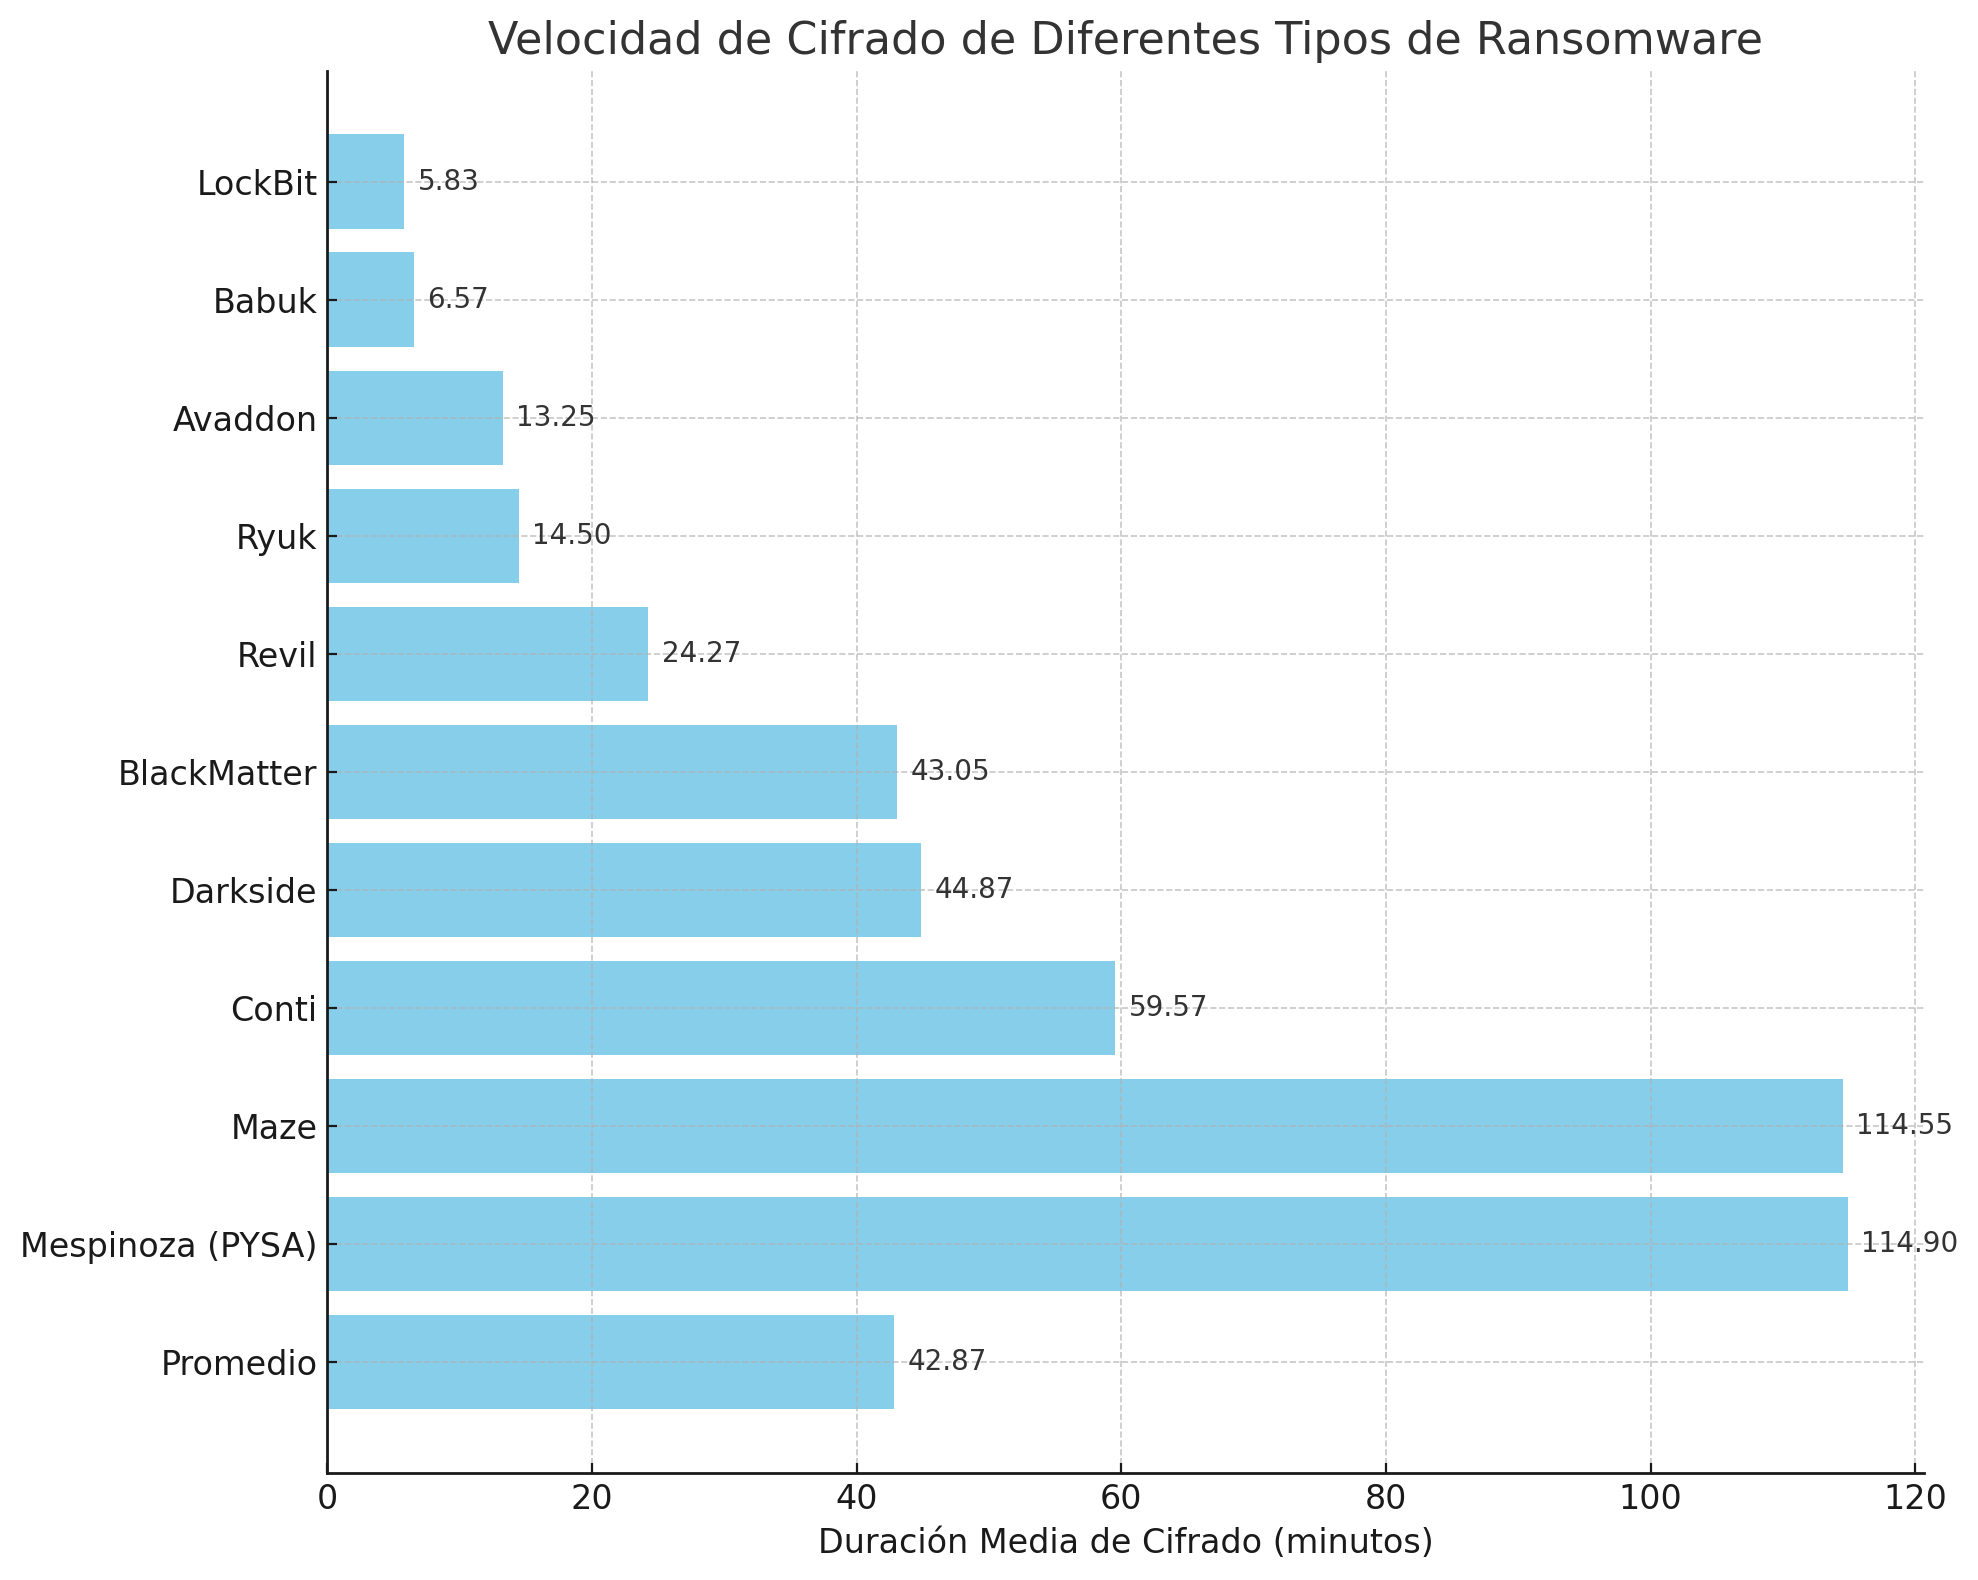
\includegraphics[width=0.8\textwidth]{imagenes/graficos/velocidad_cifrado.png} % Ajusta el nombre de archivo y la escala según sea necesario
    \caption{Comparativa de la velocidad de cifrado de distintas familias de ransomware. Este gráfico ilustra la duración media de cifrado para cada familia, destacando la eficiencia relativa de sus mecanismos de cifrado. Datos adaptados de un análisis comparativo de velocidades de cifrado de ransomware publicado por Splunk.\autocite{SplunkRansomwareSpeed}}
    \label{fig:mi-grafico}
\end{figure}                                %$$
                                                                         %$$
%%%%%%\subsection{Soluciones comerciales antiransomware}                      %$$
%%%%%%%%%
Existe una gran variedad de soluciones comerciales diseñadas para combatir el ransomware. Estas soluciones varían en enfoque, capacidades y nivel de protección ofrecido, adaptándose a diferentes necesidades y presupuestos. A continuación, se describen algunos de los tipos más comunes de soluciones anti-ransomware disponibles en el mercado.

\begin{enumerate}
  \item \textbf{Antivirus/Antimalware Avanzado:} Estas soluciones deben ser regularmente actualizadas para incorporar correcciones de seguridad, mejoras en la detección y protección contra nuevas amenazas. Existen opciones diseñadas para usuarios particulares, ofreciendo soluciones más básicas, económicas e incluso gratuitas, como AVG. También hay disponibles en el mercado opciones de pago, que incluyen soporte técnico y funciones más avanzadas, tales como Panda Premium, Norton 360, McFee, Kaspersky Anti-Ransomware o Malwarebytes Premium. Actualmente, algunos antivirus incorporan asistencia de Inteligencia Artificial, conocidos como Next-Gen Antivirus (NGAV).

  \item \textbf{Firewalls y Gateways de Seguridad:} Las soluciones de firewall y los gateways de seguridad están diseñados para filtrar el tráfico malicioso y bloquear intentos de ataques de ransomware antes de que lleguen a la red interna de una organización. Un ejemplo de esto son los firewalls de alto rendimiento de la serie Quantum Force Gateway.

  \item \textbf{Backup y Recuperación de Datos:} Mantener un sistema de backup robusto es fundamental para la recuperación de datos en caso de un ataque de ransomware. Estas soluciones permiten a las organizaciones restaurar sus sistemas a un estado anterior sin pagar el rescate.

  \item \textbf{Seguridad de Endpoint:} Las soluciones de seguridad de endpoint están diseñadas para proteger los dispositivos finales, como computadoras portátiles, estaciones de trabajo y dispositivos móviles. Pueden detectar y bloquear actividades maliciosas, incluido el ransomware, en estos dispositivos. Ejemplos de estas herramientas incluyen CyberArk Endpoint Privilege Manager (EPM) y Endpoint Detection and Response (EDR).
\end{enumerate}
                                      %$$
                                                                         %$$
\subsection{Responsabilidad Legal y Ransomware}                          %$$
\subsubsection{Marcos Legales de Protección de Datos}

Los marcos legales diseñados para regular y proteger la privacidad y seguridad de los datos personales de los individuos incluyen el Reglamento General de Protección de Datos (GDPR) en la Unión Europea y la Ley Orgánica 3/2018 de protección de datos personales y garantía de los derechos digitales (LOPDGDD) del 5 de diciembre en España. Estas leyes establecen principios y requisitos para el procesamiento de datos personales por parte de organizaciones y empresas, incluidas medidas de seguridad para prevenir la pérdida, el acceso no autorizado o la divulgación de datos.

\subsubsection{Consecuencias de un Ataque de Ransomware}

Un ataque de ransomware contra cualquier entidad, ya sea una organización o empresa, implica consecuencias no solo económicas, sino también responsabilidades legales derivadas del deber de protección de datos. Las organizaciones afectadas pueden enfrentar sanciones legales, demandas civiles y daños a su reputación debido a la falta de seguridad adecuada y la protección insuficiente de los datos.

\subsubsection{El Derecho a la Protección de Datos}

El bien jurídico protegido en todos los delitos informáticos es el derecho a la protección de datos de carácter personal, reconocido en el artículo 18.4 de la Constitución Española y por el Tribunal Constitucional en STC 292/2000, así como en el preámbulo de la LOPDGDD.

\subsubsection{Responsable del Tratamiento de Datos}

Tanto el Reglamento General de Protección de Datos (GDPR) en la Unión Europea como la Ley Orgánica de Protección de Datos (LOPDGD) en el Título V en España  se regula la figura del Responsable del Tratamiento de datos en una empresa u organización. Este responsable es la persona o entidad que determina los fines y medios del tratamiento de datos personales. Sus responsabilidades incluyen garantizar el cumplimiento de las normativas de protección de datos, implementar medidas de seguridad adecuadas para proteger la información, y responder a las solicitudes de los titulares de datos sobre sus derechos ARCO (acceso, rectificación, cancelación y oposición). Es además el responsable de notificar las brechas de seguridad de datos a la autoridad de protección de datos y, en ciertos casos, a los individuos afectados..

\subsubsection{Procedimientos y Sanciones}

En el título VIII de la LOPDGD se regula los procedimientos a seguir en caso de incumplimiento de la normativa de la protección de datos, y en el Título IX la potestad de imposición de sanciones administrativas según el tipo de infracción realizada. Las empresas también pueden recibir reclamaciones civiles por parte de los clientes por la pérdida de datos, regulado en los Artículos 1101 y 1902 del Código Civil.

\subsubsection{Denuncia de Ataques de Ransomware}

Cualquier ataque de ransomware debe ser denunciado a las fuerzas de seguridad del estado, ya que comprende delitos penalmente castigados como daños informáticos, blanqueo de capitales, intrusismo, estafa, pertenencia a organización criminal y delitos contra la intimidad.
                                  %$$
                                                                         %$$
%************************************************************************%$$
%                                                                        %$$
%                      FIN de Estado del arte                            %$$
%                                                                        %$$
%========================================================================%$$



%========================================================================%$$
%                                                                        %$$
%                                Bacula                                  %$$
%                                                                        %$$
%========================================================================%$$
                                                                         %$$
\section{Bacula}                                                         %$$
La continua adaptación del ransomware frente a las medidas de defensa subraya la urgente necesidad de soluciones de backup robustas y flexibles. En este contexto, Bacula emerge como una herramienta prometedora, destacándose por su configuración adaptable y su apoyo a prácticas avanzadas de backup. Este análisis se enfoca en el estado actual de Bacula, evaluando su implementación y eficacia como parte de una estrategia de ciberseguridad integral, brindando una perspectiva sobre el fortalecimiento de la resiliencia organizacional frente a la amenaza del ransomware.\medskip

Bacula, un sistema de backup, recuperación y verificación de datos a través de la red, ofrece una solución integral para la gestión de backups. Su arquitectura se compone de varios componentes clave, incluyendo el Director, el Cliente, y el Almacenamiento, trabajando en conjunto para asegurar la integridad y la disponibilidad de los datos\autocite{bacula2023current}.

\medskip

\subsection{Características Implementadas}

\medskip
Las capacidades actuales de Bacula abarcan:

\begin{itemize}
  \item \textbf{Control de Trabajos:} \begin{itemize} \item Bacula ofrece un control exhaustivo sobre los backups, permitiendo programaciones automáticas, ejecución simultánea de múltiples trabajos y secuenciación basada en prioridades.\end{itemize}
  \item \textbf{Seguridad:}  \begin{itemize} \item Incluye verificación de archivos, autenticación CRAM-MD5, encriptación TLS y de datos, así como la computación de firmas digitales.\end{itemize}
  \item \textbf{Restauración Avanzada:} \begin{itemize} \item Bacula posibilita la restauración de archivos de manera interactiva, la recuperación completa del sistema y la restauración del catálogo de backups.\end{itemize}
  \item \textbf{Gestión de Catálogo SQL:}  \begin{itemize} \item Soporta bases de datos MySQL, PostgreSQL y SQLite, facilitando una amplia gestión de los datos de backup.\end{itemize}
  \item \textbf{Administración de Volúmenes y Piscinas:} Permite una gestión flexible de los medios de almacenamiento, incluyendo la migración de datos y el soporte para dispositivos auto-cargadores.
  \item \textbf{Soporte Multiplataforma:}  \begin{itemize} \item Compatible con una variedad de sistemas operativos, ofrece compresión GZIP y mantiene la coherencia de backups en sistemas Win32 mediante VSS.\end{itemize}
\end{itemize}

\subsection{Restricciones Actuales y Limitaciones de Diseño}


A pesar de su robustez, Bacula enfrenta limitaciones, como la restauración compleja de trabajos simultáneos y la transición entre arquitecturas significativamente diferentes. Además, el diseño impone límites en la longitud de nombres y en la entrada de comandos en algunas herramientas independientes.\medskip

Específicamente, la programación interna de Bacula, aunque eficiente, presenta limitaciones en entornos donde la concurrencia de trabajos es crítica. El sistema de colas FCFS y el manejo estático de prioridades pueden resultar en ineficiencias, como el efecto convoy y la posible inanición de trabajos de baja prioridad. Estos desafíos subrayan la necesidad de enfoques de programación más dinámicos y adaptativos.\medskip

La implementación y evaluación de Bacula en escenarios simulados de ransomware proporcionan una valiosa oportunidad para examinar su efectividad dentro de una estrategia de ciberseguridad comprensiva. A través de este trabajo, se busca no solo explorar la robustez de Bacula frente a la amenaza del ransomware, sino también identificar áreas de mejora que puedan fortalecer aún más la resiliencia organizacional.\medskip
                                                    %$$
                                                                         %$$
%************************************************************************%$$
%                                                                        %$$
%                          FIN de Bacula                                 %$$
%                                                                        %$$
%========================================================================%$$





%========================================================================%$$
%                                                                        %$$
%                    Arquitectura de nuestro sistema                     %$$
%                                                                        %$$
%========================================================================%$$
                                                                         %$$
\section{Arquitectura de nuestro sistema}                                %$$
La arquitectura propuesta para el TFM incluye los siguientes servidores:

\begin{enumerate}
    \item \textbf{Servidor Bacula en Debian}: Este servidor actuará como el Director de Bacula y alojará el Catálogo en una base de datos PostgreSQL.
    \item \textbf{Servidor Debian para Prácticas de Archivos}: Actuará como cliente de Bacula para realizar prácticas de respaldo de archivos.
    \item \textbf{Servidor Debian para Prácticas con Bases de Datos}: Se utilizará para prácticas de respaldo de bases de datos, funcionando como otro cliente de Bacula.
    \item \textbf{Servidor Windows para Prácticas de Archivos}: Este servidor funcionará como cliente en un entorno Windows, demostrando la capacidad de Bacula para trabajar en entornos mixtos.
\end{enumerate}







\begin{figure}[H]
    \centering
    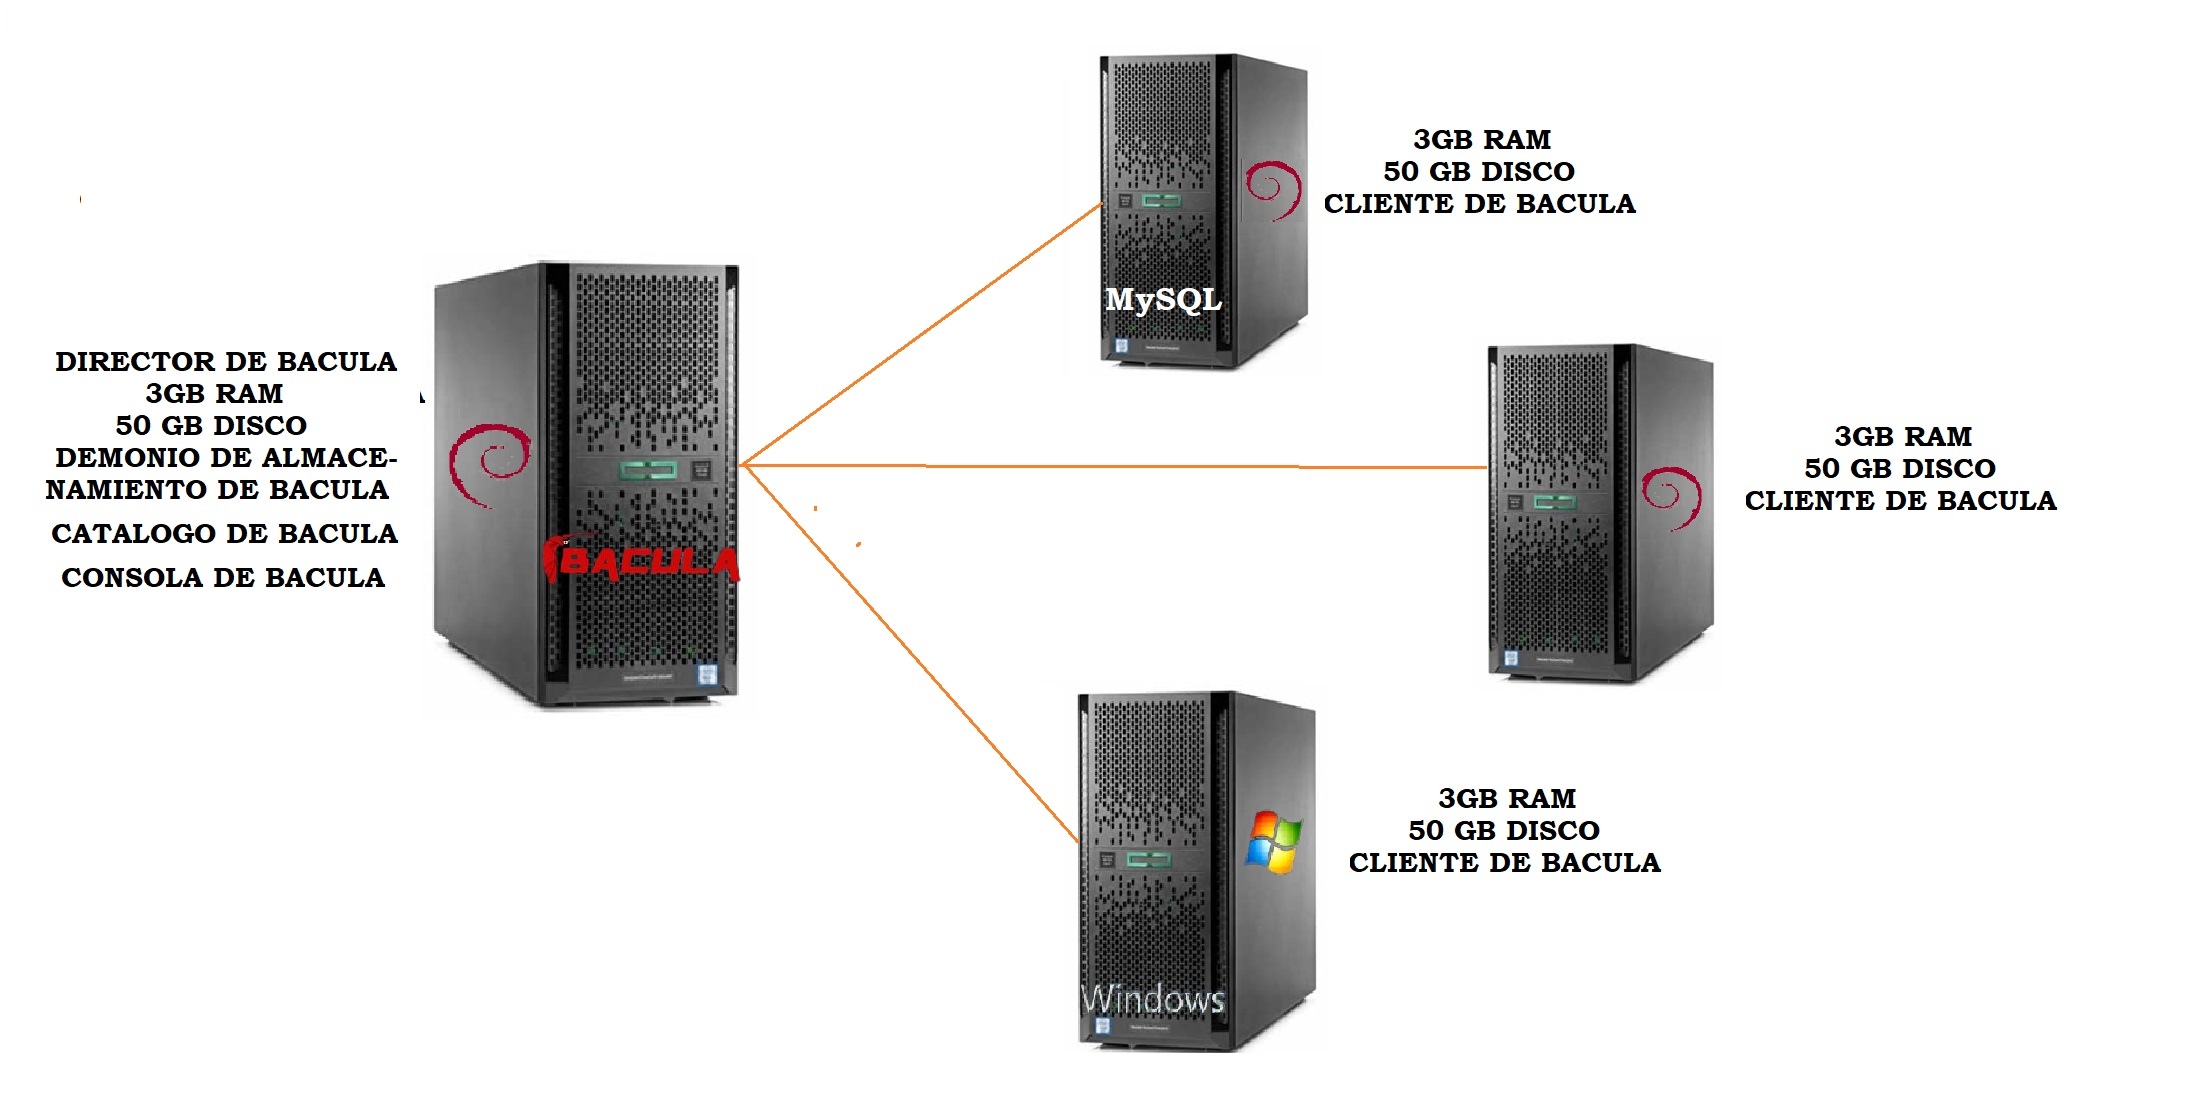
\includegraphics[width=1\textwidth]{imagenes/graficos/BACULA.jpg} % Ajusta el nombre de archivo y la escala según sea necesario
    \caption{Diagrama de la arquitectura de prueba.}
    \label{fig:mi-grafico}
\end{figure}





\subsection{Implementación de los Demonios de Bacula}

La arquitectura de Bacula está diseñada para proporcionar una solución robusta y flexible para la gestión de copias de seguridad en entornos distribuidos. Cada demonio de Bacula juega un papel crítico en este ecosistema, asegurando la eficiencia y seguridad en la realización de backups y restauraciones. A continuación, se describe la implementación de cada demonio dentro de nuestra arquitectura específica.

\subsubsection{Director de Bacula}

El \textbf{Director de Bacula} es el componente central de nuestra arquitectura de backups, encargado de coordinar todas las operaciones de backup y restauración. Este demonio está configurado en nuestro \textit{servidor Debian principal}, el cual actúa como el cerebro del sistema de backups, gestionando tanto la lógica de las operaciones como las políticas y programaciones de los backups.

\begin{itemize}
    \item \textbf{Ubicación:} Servidor Debian principal.
\end{itemize}

\subsubsection{Demonio de Almacenamiento de Bacula}

El \textbf{Demonio de Almacenamiento de Bacula} gestiona los dispositivos físicos o virtuales donde se almacenan los backups. Para optimizar el rendimiento y la escalabilidad de nuestro sistema, este demonio se implementa tanto en el servidor Debian principal como en un \textit{servidor de almacenamiento dedicado}, proporcionando así redundancia y flexibilidad en las opciones de almacenamiento.

\begin{itemize}
    \item \textbf{Ubicaciones:} Servidor Debian principal y servidor de almacenamiento dedicado.
\end{itemize}

\subsubsection{Catálogo de Bacula}

El \textbf{Catálogo de Bacula}, implementado usando \textit{PostgreSQL}, ofrece un índice detallado y metadatos de todas las copias de seguridad y restauraciones realizadas. Este componente es crucial para la gestión eficiente de los backups, permitiendo búsquedas rápidas y la administración de los datos almacenados. El Catálogo se aloja en el \textit{servidor Debian principal}, junto al Director de Bacula, para facilitar la comunicación y el acceso a los datos.

\begin{itemize}
    \item \textbf{Ubicación:} Servidor Debian principal, con PostgreSQL como sistema de gestión de base de datos.
\end{itemize}

\subsubsection{Consola de Bacula}

La \textbf{Consola de Bacula} proporciona la interfaz de usuario para la gestión y monitoreo de las operaciones de backups y restauraciones. Para garantizar un acceso administrativo conveniente, la consola se instala en el \textit{servidor Debian principal} y también está disponible para los administradores a través de sus estaciones de trabajo personales, permitiendo la gestión remota del sistema de backups.

\begin{itemize}
    \item \textbf{Ubicaciones:} Servidor Debian principal y estaciones de trabajo de administradores.
\end{itemize}

\subsubsection{Cliente de Bacula}

El \textbf{Cliente de Bacula} o File Daemon se instala en cada sistema que requiere ser respaldado. En nuestra arquitectura, esto incluye el \textit{servidor Debian para prácticas de archivos}, el \textit{servidor Debian para prácticas con bases de datos}, y el \textit{servidor Windows para prácticas de archivos}. Estos clientes son responsables de enviar los datos al Demonio de Almacenamiento bajo la dirección del Bacula Director.

\begin{itemize}
    \item \textbf{Ubicaciones:} Servidor Debian para prácticas de archivos, servidor Debian para prácticas con bases de datos, y servidor Windows para prácticas de archivos.
\end{itemize}

















\subsection{Tipos de backup}
En la gestión de copias de seguridad con Bacula, como en muchos otros sistemas de backups, se utilizan diferentes estrategias para optimizar el proceso de almacenamiento, reducir el tiempo necesario para realizar las copias de seguridad y facilitar la recuperación de los datos. Estas estrategias se pueden combinar para crear un plan de backups robusto y eficiente. Las cuatro estrategias principales son: completa (full), diferencial, incremental y mixta.

\subsubsection{Completa (Full)}
En una copia de seguridad completa, se copian todos los archivos seleccionados en el sistema. Es la base sobre la cual se realizan las demás estrategias de copia de seguridad, ya que cualquier método de restauración comienza con una copia completa.

\textbf{Escenarios recomendados}: La copia de seguridad completa es ideal para iniciar un ciclo de backups, asegurando que se tenga al menos una versión íntegra de todos los datos. Se recomienda realizar copias de seguridad completas periódicamente, dependiendo del tamaño de los datos y de la capacidad de almacenamiento, por ejemplo, semanalmente o mensualmente.

\subsubsection{Diferencial}
Una copia de seguridad diferencial guarda los cambios realizados desde la última copia de seguridad completa. Cada copia diferencial incluye todos los cambios acumulados desde la última copia completa, lo que significa que su tamaño puede crecer considerablemente con el tiempo hasta que se realiza otra copia completa.

\textbf{Escenarios recomendados}: Esta estrategia es útil cuando se desean minimizar los tiempos de restauración manteniendo un equilibrio con el espacio de almacenamiento utilizado. Es ideal para entornos donde los datos cambian con frecuencia, pero donde realizar una copia completa a menudo no es viable. Se pueden programar copias diferenciales diariamente o semanalmente, según la tasa de cambio de los datos.

\subsubsection{Incremental}
Las copias de seguridad incrementales sólo almacenan los datos que han cambiado desde la última copia de seguridad de cualquier tipo (sea completa, diferencial o incremental). Esto minimiza el tiempo necesario para realizar la copia de seguridad y reduce el espacio de almacenamiento requerido.

\textbf{Escenarios recomendados}: Esta estrategia es excelente para datos que cambian diariamente pero en los que el volumen total de los cambios es relativamente pequeño. Permite realizar copias de seguridad frecuentes, como diarias, con un mínimo impacto en los recursos de almacenamiento y en el rendimiento del sistema.

\subsubsection{Mixta}
La estrategia mixta combina las copias de seguridad completas, diferenciales e incrementales de una manera que mejor se adapte a las necesidades específicas de recuperación y almacenamiento de datos de una organización. Un ejemplo común de una estrategia mixta es realizar una copia completa mensualmente, copias diferenciales semanalmente y copias incrementales diariamente.

\textbf{Escenarios recomendados}: Esta estrategia es ideal para entornos con una gran cantidad de datos y requisitos complejos de recuperación. Permite maximizar la eficiencia del almacenamiento y minimizar los tiempos de restauración ajustando la frecuencia de los diferentes tipos de copias de seguridad según las necesidades específicas y la dinámica de cambios de los datos.

\subsubsection{Implementación de Estrategias de Backups en Bacula}

Para evaluar exhaustivamente las capacidades de Bacula en la gestión de copias de seguridad, se implementarán y probarán cuatro estrategias principales: completa, diferencial, incremental y mixta. La finalidad es determinar la eficacia, eficiencia y aplicabilidad de cada estrategia en distintos escenarios. A continuación, se detalla el proceso de implementación y evaluación para cada estrategia de backup.


\textbf{Backup Completo}

Inicialmente, se realizará un backup completo de todos los datos en los servidores configurados. Este paso es fundamental, ya que establece la base sobre la cual se construirán las demás estrategias de backups.

\begin{enumerate}
    \item Ejecución de la copia de seguridad completa en cada servidor para capturar todos los datos existentes.
    \item Documentación del tiempo requerido y del espacio de almacenamiento consumido por esta operación.
    \item Análisis de la eficiencia del proceso de backup completo en términos de duración y uso del almacenamiento.
\end{enumerate}

\textbf{Backup Diferencial
}
Posteriormente, se implementará la estrategia de backup diferencial para entender cómo afecta la acumulación de cambios desde el último backup completo.

\begin{enumerate}
    \item Modificación de una parte significativa de los datos para simular la actividad regular.
    \item Realización de backups diferenciales para capturar los cambios desde el último backup completo.
    \item Evaluación del incremento en tiempo y almacenamiento en comparación con el backup completo.
\end{enumerate}

\textbf{Backup Incremental}
La estrategia de backup incremental se probará para observar su eficiencia en el manejo de cambios diarios mínimos.

\begin{enumerate}
    \item Introducción de cambios adicionales en los datos después del último backup (completo o diferencial).
    \item Ejecución de backups incrementales que solo capturan los cambios desde el último backup de cualquier tipo.
    \item Comparación y análisis del desempeño y la optimización del almacenamiento frente a las estrategias anteriores.
\end{enumerate}

\textbf{Estrategia Mixta}

Por último, se diseñará e implementará una estrategia mixta que combine los métodos completo, diferencial e incremental, ajustándolos a un calendario que maximice la eficiencia del almacenamiento y la rapidez en la restauración.

\begin{enumerate}
    \item Diseño de un esquema de backups que incluya backups completos mensuales, backups diferenciales semanales y backups incrementales diarios.
    \item Implementación del esquema durante un período de prueba para evaluar la cobertura y eficiencia.
    \item Documentación exhaustiva de los resultados, incluyendo el rendimiento, la eficiencia del almacenamiento y la facilidad de recuperación.
\end{enumerate}                                        %$$
                                                                         %$$
%************************************************************************%$$
%                                                                        %$$
%                FIN de Arquitectura de nuestro sistema                  %$$
%                                                                        %$$
%========================================================================%$$



\newpage

% implementacion
\section{Implementación de Bacula}                                






\subsection{Configuración de Backups en Bacula}

Configurar un backup en Bacula implica varios pasos críticos que aseguran que los datos importantes sean respaldados de manera eficiente y segura. A continuación, se detallan los pasos necesarios para configurar un backup dentro del sistema Bacula:

\begin{enumerate}
    \item \textbf{Definición de los Datos a Respaladar:} El primer paso en la configuración de un backup es especificar qué datos serán incluidos. Esto se realiza mediante la creación de un \textit{FileSet}, el cual incluye una lista de archivos y directorios que Bacula deberá respaldar. También se pueden especificar exclusiones dentro del mismo \textit{FileSet} para omitir archivos no necesarios o temporales.
    
    \item \textbf{Programación del Backup:} El siguiente paso es definir cuándo se realizarán los backups. Esto se configura a través de una \textit{Schedule} en Bacula, donde se pueden especificar diferentes políticas de tiempo, como backups diarios, semanales o mensuales. Cada \textit{Schedule} puede incluir múltiples eventos para manejar distintos tipos de backups (completo, incremental, diferencial) en distintos momentos.
    
    \item \textbf{Selección del Cliente:} Bacula permite realizar backups de múltiples máquinas. En este paso, se debe agregar el cliente o los clientes que serán parte del backup. Esto se define en una sección llamada \textit{Client}, donde se especifica la dirección de la máquina y otros parámetros necesarios para la comunicación y ejecución de los backups.
    
    \item \textbf{Creación del Job:} Un \textit{Job} en Bacula es la entidad que encapsula toda la información necesaria para ejecutar un backup. Incluye la vinculación del \textit{FileSet}, el \textit{Client}, y la \textit{Schedule}. Además, se debe especificar el tipo de backup y el destino del mismo, como puede ser un disco o cinta. Aquí también se definen las políticas de retención y otras opciones avanzadas.
    
    \item \textbf{Ejecución del Job:} Finalmente, una vez configurado, el job puede ser ejecutado manualmente a través de la consola de Bacula o automáticamente según la programación establecida. Durante la ejecución, Bacula gestionará la transferencia de datos desde el cliente al medio de almacenamiento especificado, siguiendo las políticas definidas en el job.
\end{enumerate}

Este proceso asegura que los datos importantes estén protegidos y que el proceso de recuperación pueda ser llevado a cabo de manera eficiente en caso de pérdida de datos o desastres.


\subsubsection{Definición de Conjuntos de Archivos (File Sets)}
Para iniciar la configuración de backups, primero definimos los conjuntos de archivos que especifican qué datos se deben respaldar. En Bacula, esto se realiza mediante la creación de File Sets, que pueden incluir diversos directorios y tipos de archivos.

\begin{figure}[H]
    \centering
    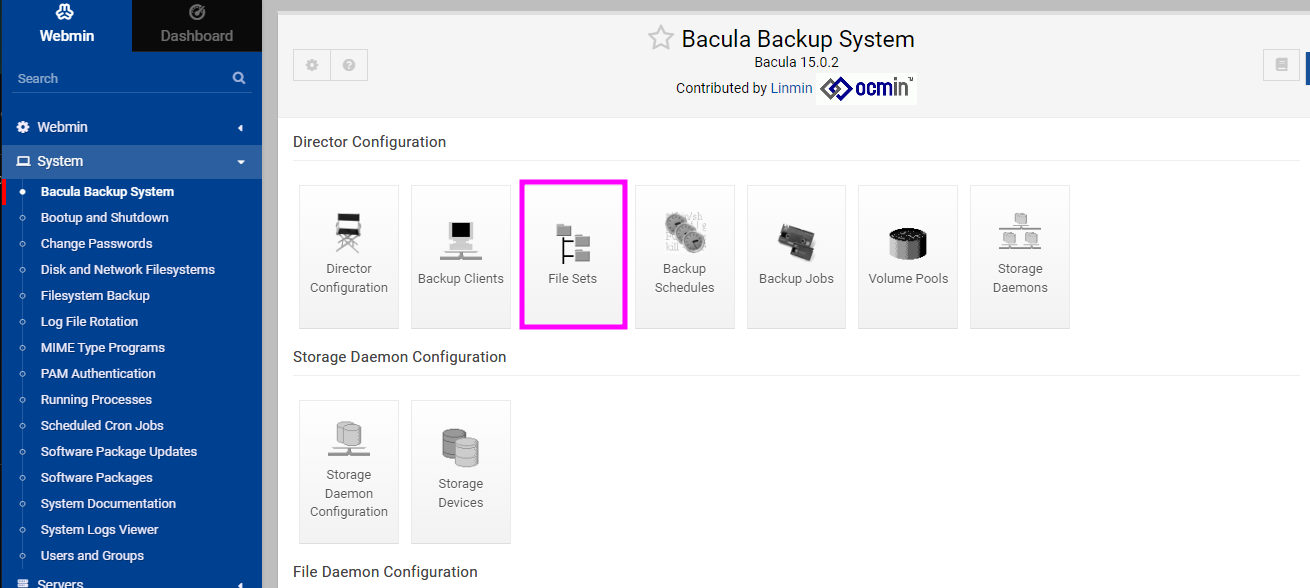
\includegraphics[width=0.5\linewidth]{instalacionBacula/filesetwebmin.png}
    \caption{Creación de un nuevo File Set en Webmin}
\end{figure}




\begin{minipage}[t]{0.45\textwidth}
    \vspace{0pt} % Alinea la parte superior de la minipágina con lo que esté al lado
    Durante la instalación, se crean algunos File Sets por defecto. Sin embargo, para fines específicos o para asegurar la integridad de datos críticos, podemos crear File Sets personalizados como se muestra a continuación:
   

    \end{minipage}%
    \hfill % Añade espacio entre las dos minipáginas si es necesario
    \begin{minipage}[t]{0.45\textwidth}
    \vspace{0pt} % Alinea la parte superior de la minipágina con lo que esté al lado
    \centering % Centra el contenido de la minipágina
      
    \begin{figure}[H]
        \centering
        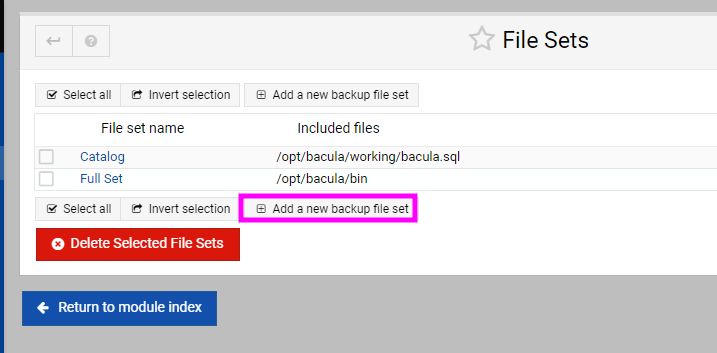
\includegraphics[width=0.95\linewidth]{instalacionBacula/cpropiofileset.png}
        \caption{Visualización de File Sets existentes}
    \end{figure}
    \end{minipage}


\smallskip






\begin{minipage}[t]{0.45\textwidth}
    \vspace{0pt} % Alinea la parte superior de la minipágina con lo que esté al lado
    En la creación de un File Set, es fundamental configurar adecuadamente las opciones disponibles, como el tipo de firma de archivo (por ejemplo, MD5 para verificación de integridad), los directorios a respaldar, y los niveles de compresión.
   

    \end{minipage}%
    \hfill % Añade espacio entre las dos minipáginas si es necesario
    \begin{minipage}[t]{0.45\textwidth}
    \vspace{0pt} % Alinea la parte superior de la minipágina con lo que esté al lado
    \centering % Centra el contenido de la minipágina
      
    
\begin{figure}[H]
    \centering
    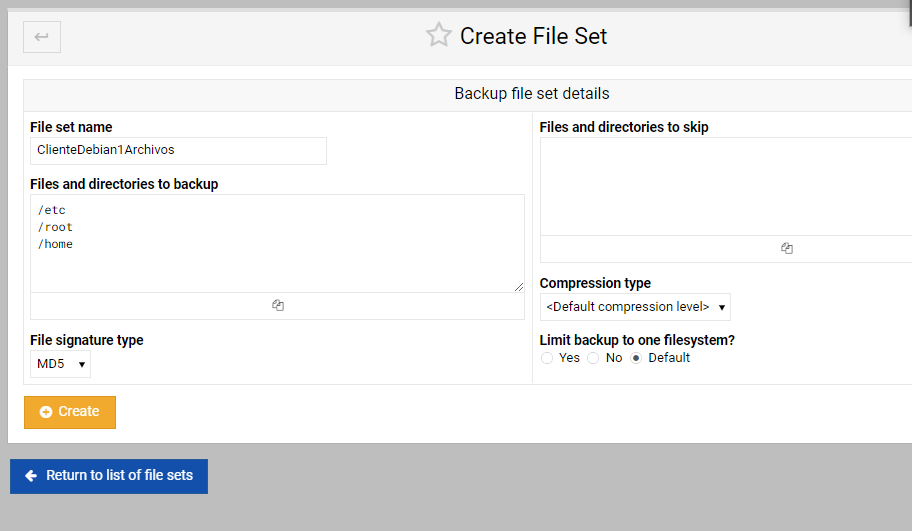
\includegraphics[width=0.95\linewidth]{instalacionBacula/createrfilesett.png}
    \caption{Configuración detallada de un File Set}
\end{figure}
    \end{minipage}


\smallskip














\subsubsection{Programación de Backups}






\begin{minipage}[t]{0.45\textwidth}
    \vspace{0pt} % Alinea la parte superior de la minipágina con lo que esté al lado
    El siguiente paso es definir cuándo se realizarán los backups, lo cual se configura mediante las programaciones de backup (schedules). Bacula permite definir múltiples programaciones para adaptarse a diferentes necesidades operativas.
   

    \end{minipage}%
    \hfill % Añade espacio entre las dos minipáginas si es necesario
    \begin{minipage}[t]{0.45\textwidth}
    \vspace{0pt} % Alinea la parte superior de la minipágina con lo que esté al lado
    \centering % Centra el contenido de la minipágina
      
    

    \begin{figure}[H]
        \centering
        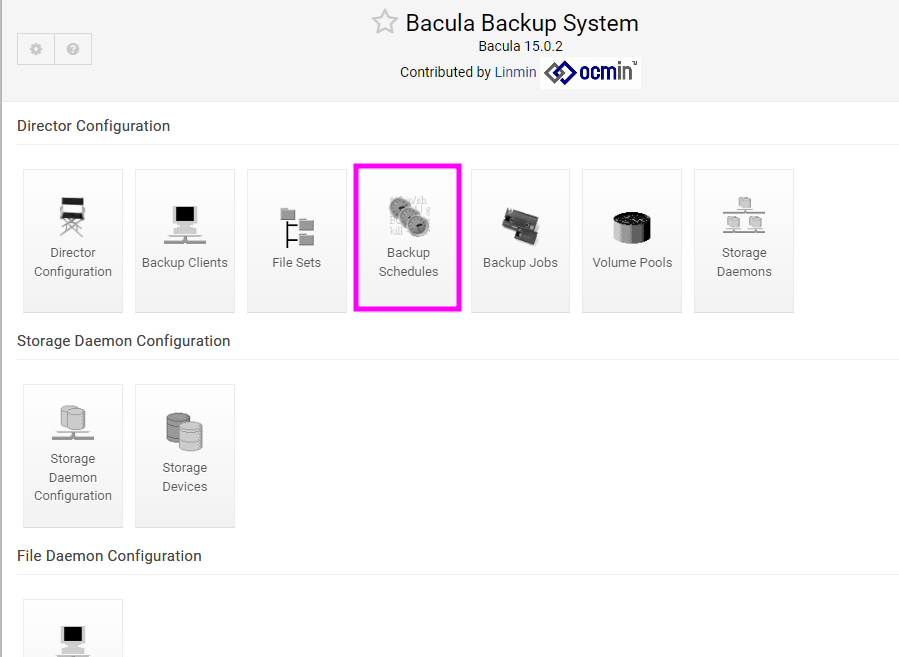
\includegraphics[width=0.95\linewidth]{instalacionBacula/schedule.png}
        \caption{Programaciones de backup existentes}
    \end{figure}
    \end{minipage}


\smallskip





Para cada necesidad específica, se puede crear una nueva programación que detalle los niveles de backup (completo, diferencial, incremental), así como la frecuencia con la que estos deben ejecutarse.

\begin{figure}[H]
    \centering
    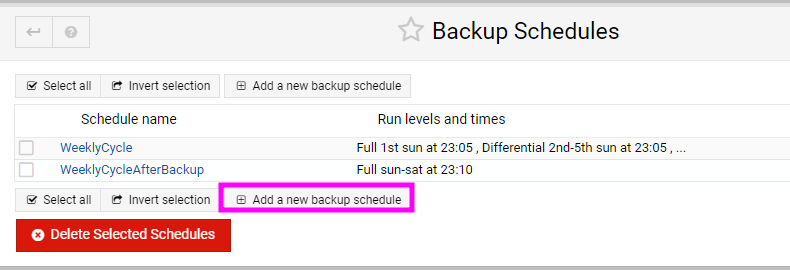
\includegraphics[width=0.5\linewidth]{instalacionBacula/newBackupSchedules.png}
    \caption{Creación de una nueva programación de backup}
\end{figure}

En la configuración de una programación, se definen los tiempos específicos y los tipos de backup, asegurando que los datos se respalden en los intervalos y formas adecuados.

\begin{figure}[H]
    \centering
    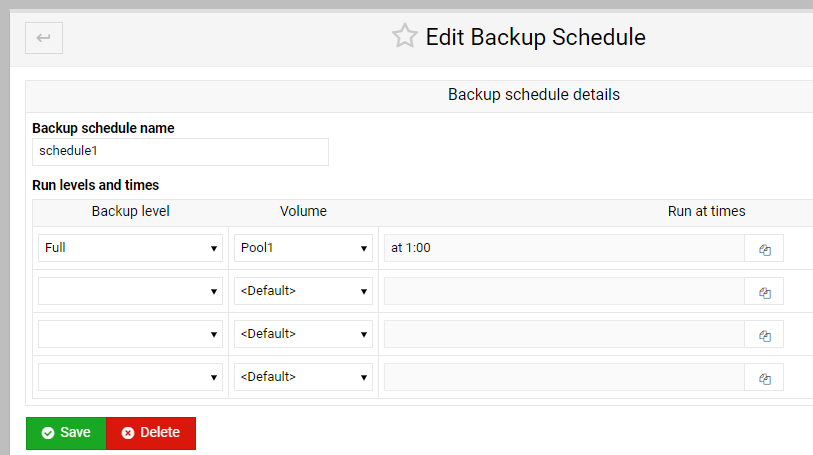
\includegraphics[width=0.5\linewidth]{instalacionBacula/editbuckupschedule.png}
    \caption{Edición de una programación de backup}
\end{figure}






\subsubsection{Clientes Respaldados}

Ahora necesitamos selecionar a quien vamos a backupear
\begin{figure}[H]
    \centering
    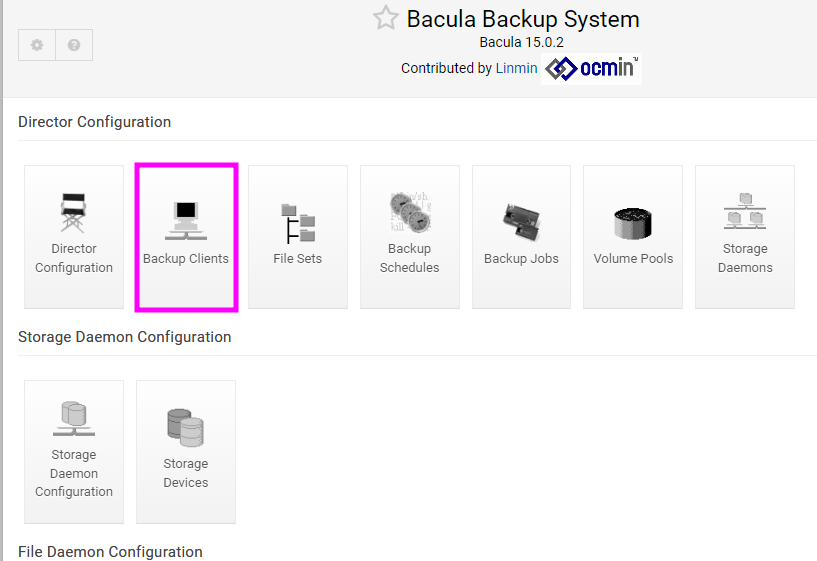
\includegraphics[width=0.5\linewidth]{instalacionBacula/asdasdas.png}
    \caption{Clientes de respaldo.}
\end{figure}

Después de definir los \textit{filesets} y los \textit{schedules}, procedemos a configurar los clientes que serán respaldados y a crear los jobs de respaldo.

\text{Añadiendo Clientes de Respaldo}

Inicialmente, el sistema tiene configurado al servidor Bacula para auto-respaldarse. Para añadir nuevos clientes:

\begin{figure}[H]
    \centering
    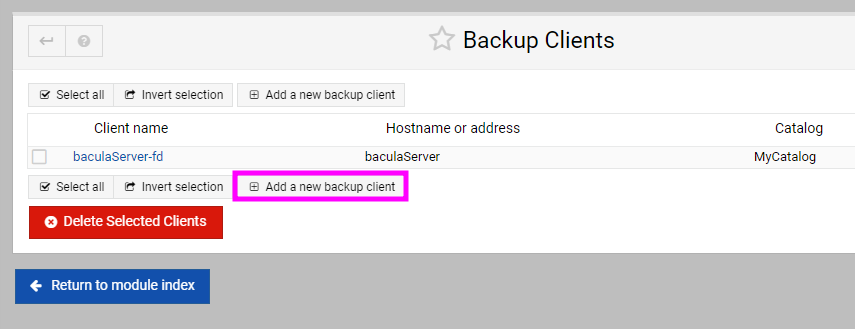
\includegraphics[width=0.5\linewidth]{instalacionBacula/addnewbuckupclient.png}
    \caption{Interfaz para añadir un nuevo cliente de respaldo.}
\end{figure}

Configuramos los detalles del nuevo cliente a respaldar:





\begin{minipage}[t]{0.45\textwidth}
    \vspace{0pt} % Alinea la parte superior de la minipágina con lo que esté al lado
    \begin{itemize}
        \item \textbf{Nombre del Cliente FD:} baculaCliente-fd
        \item \textbf{Contraseña FD de Bacula:} 
        \item \textbf{Hostname o dirección IP:} 192.168.1.116
        \item \textbf{Puerto FD de Bacula:} 9102
        \item \textbf{Catálogo a usar:} MyCatalog
        \item \textbf{Prune de trabajos y archivos caducados:} Sí
        \item \textbf{Tiempo de retención de archivos de respaldo:} 1 mes
    \end{itemize}

    \end{minipage}%
    \hfill % Añade espacio entre las dos minipáginas si es necesario
    \begin{minipage}[t]{0.45\textwidth}
    \vspace{0pt} % Alinea la parte superior de la minipágina con lo que esté al lado
    \centering % Centra el contenido de la minipágina
      
    

    
\begin{figure}[H]
    \centering
    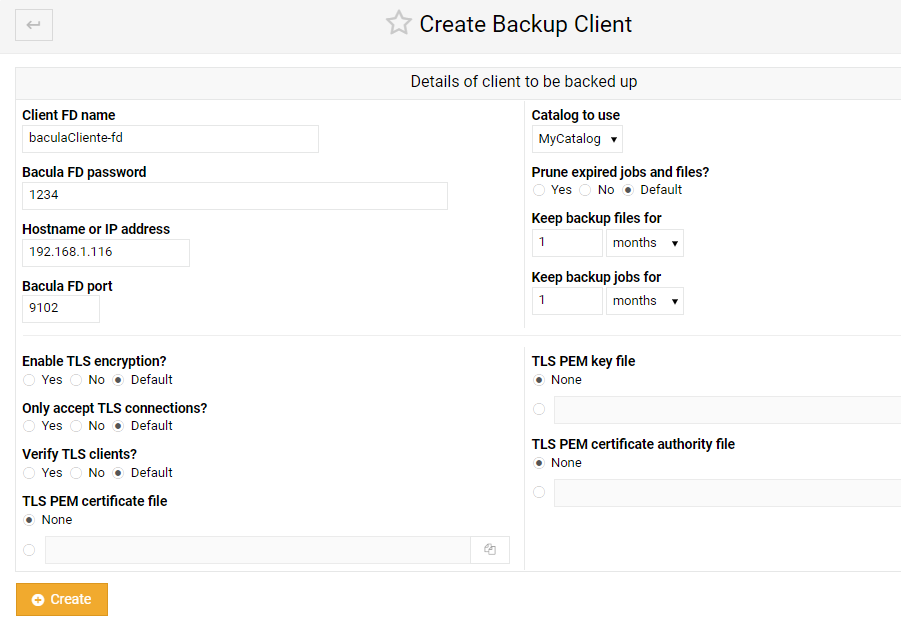
\includegraphics[width=0.95\linewidth]{instalacionBacula/detalesclienteparabuckup.png}
    \caption{Detalles del cliente a respaldar.}
\end{figure}
    \end{minipage}


\smallskip






\subsubsection{Creación y Configuración de Jobs de Respaldo}
Ahora podemos crear y ejecutar un job:

\begin{figure}[H]
    \centering
    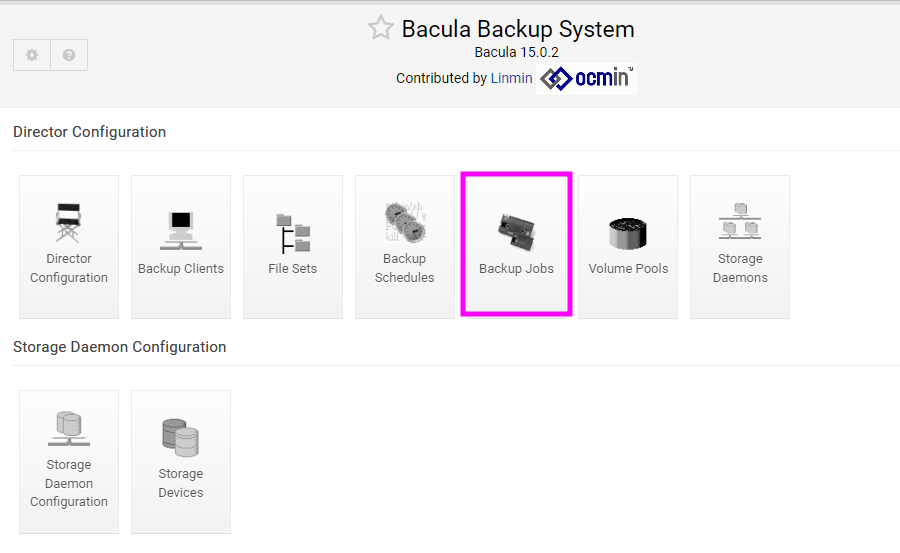
\includegraphics[width=0.5\linewidth]{instalacionBacula/createJOB.png}
    \caption{Crear un job.}
\end{figure}
Procedemos a crear un nuevo job de respaldo que utilizará las configuraciones establecidas:

\begin{figure}[H]
    \centering
    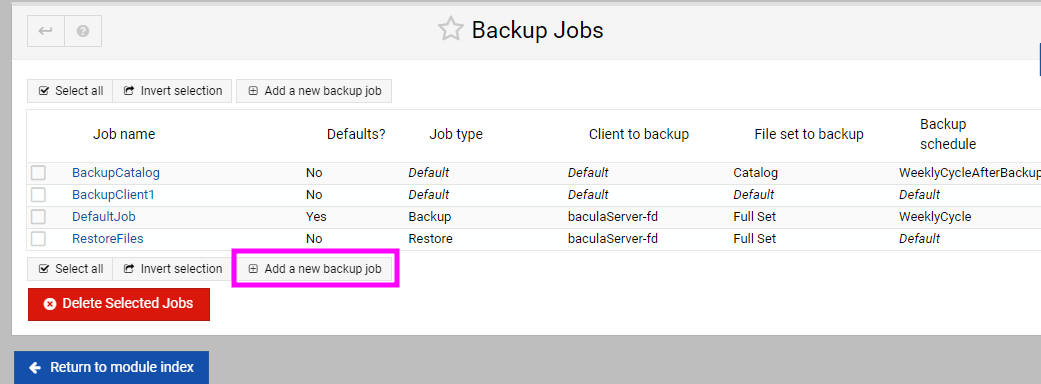
\includegraphics[width=0.5\linewidth]{instalacionBacula/createnewjob.png}
    \caption{Creación de un nuevo job de respaldo.}
\end{figure}

Los detalles para configurar el job de respaldo son:


\begin{minipage}[t]{0.45\textwidth}
    \vspace{0pt} % Alinea la parte superior de la minipágina con lo que esté al lado
    \begin{itemize}
        \item \textbf{Nombre del Job de Respaldo:} ClienteDebian1BackupJob
        \item \textbf{Tipo de Job:} Backup
        \item \textbf{Nivel de Respaldo:} Completo
        \item \textbf{Cliente a Respaldar:} baculaCliente-fd
        \item \textbf{Set de Archivos:} ClienteDebian1Archivos
        \item \textbf{Programación:} schedule1
        
    \end{itemize}

    \end{minipage}%
    \hfill % Añade espacio entre las dos minipáginas si es necesario
    \begin{minipage}[t]{0.45\textwidth}
    \vspace{0pt} % Alinea la parte superior de la minipágina con lo que esté al lado
    \centering % Centra el contenido de la minipágina
      
    

    \begin{figure}[H]
        \centering
        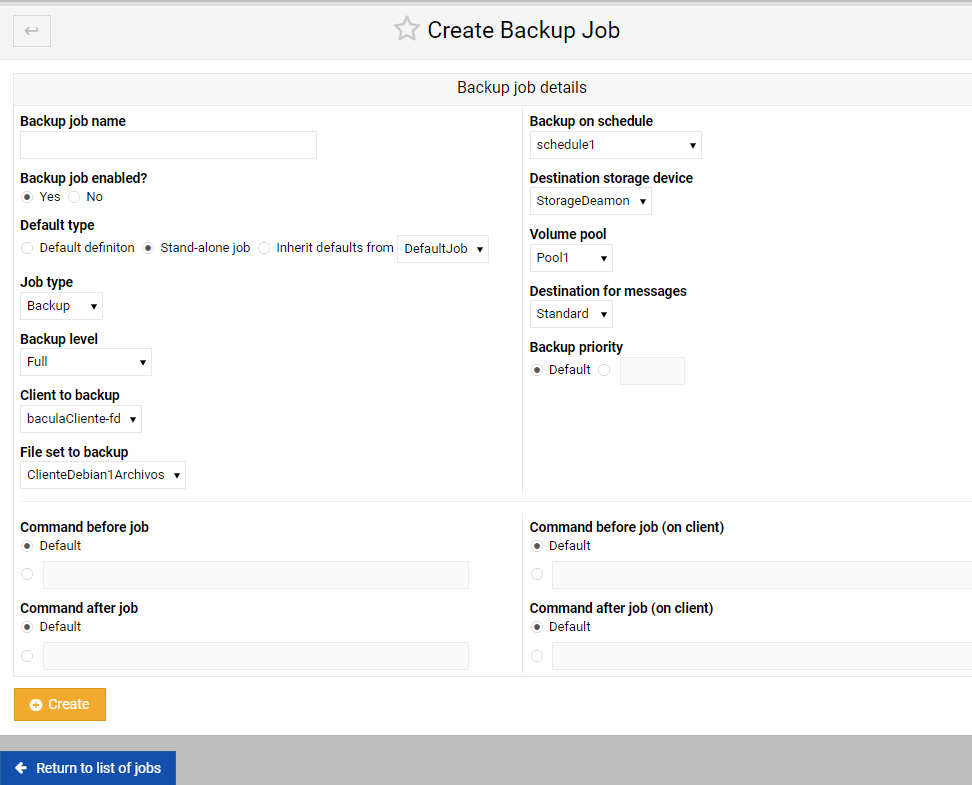
\includegraphics[width=0.95\linewidth]{instalacionBacula/Backupjobdetails.png}
        \caption{Detalles del job de respaldo configurado.}
    \end{figure}
    \end{minipage}


\smallskip

\begin{itemize}
    \item \textbf{Dispositivo de Almacenamiento Destino:} StorageDaemon
    \item \textbf{Pool de Volumen:} Pool1
    \item \textbf{Prioridad del Respaldo:} Predeterminada
\end{itemize}






\subsubsection{Ejecución de un Job de Respaldo}

Finalmente, ejecutamos el job de respaldo de manera manual para validar la configuración:

\begin{figure}[H]
    \centering
    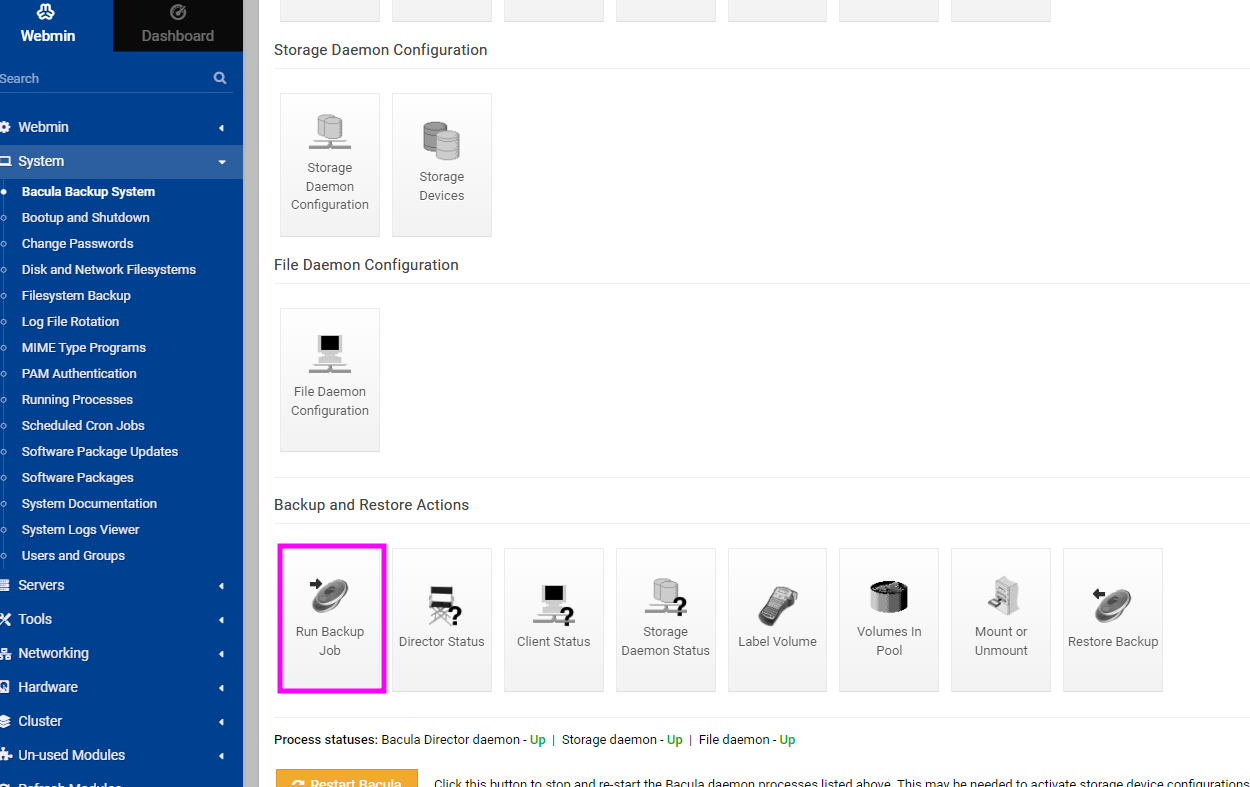
\includegraphics[width=0.5\linewidth]{instalacionBacula/runbackupjonbb.png}
    \caption{Interfaz para ejecutar un job de respaldo.}
\end{figure}

Seleccionamos el job deseado y hacemos clic en \textit{Backup Now}:

\begin{figure}[H]
    \centering
    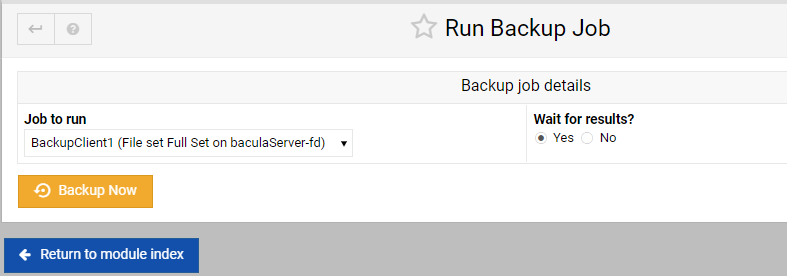
\includegraphics[width=0.5\linewidth]{instalacionBacula/backupnoww.png}
    \caption{Ejecución inmediata de un job de respaldo.}
\end{figure}

Tras la ejecución, el sistema nos proporciona un resumen detallado del proceso de respaldo:

\begin{figure}[H]
    \centering
    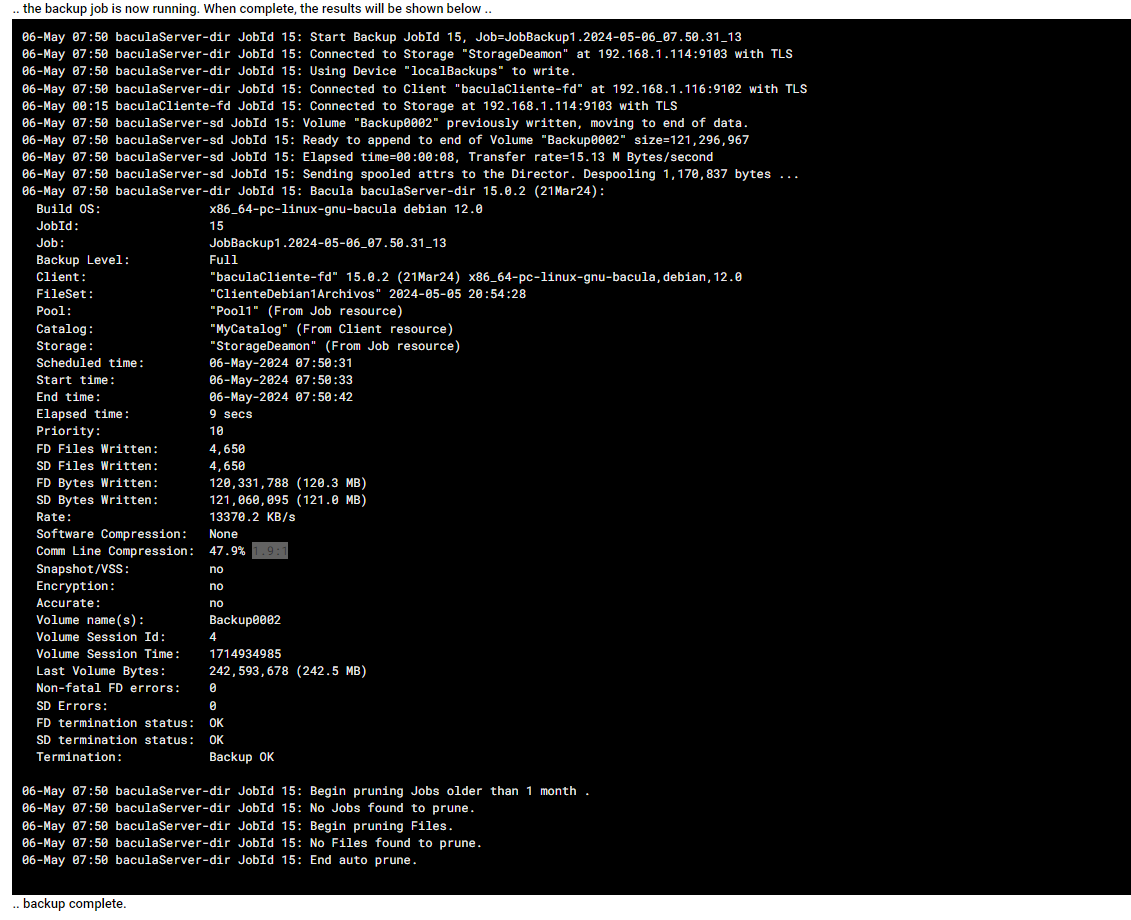
\includegraphics[width=0.5\linewidth]{instalacionBacula/salidajob1.png}
    \caption{Resultado detallado del job de respaldo ejecutado.}
\end{figure}

Con esto concluimos la configuración básica y operación del sistema de respaldos Bacula dentro de nuestra infraestructura.


\subsection{Restore en un Cliente Linux}

Para ilustrar el proceso de restauración, he creado cinco archivos de texto y he calculado el \texttt{md5sum} de dos de ellos que luego serán eliminados y restaurados.

\begin{figure}[H]
    \centering
    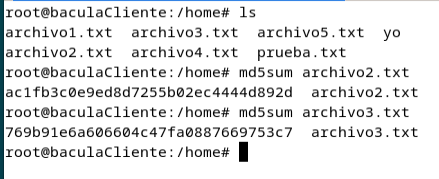
\includegraphics[width=0.5\linewidth]{instalacionBacula/5ARCHIVOS.png}
    \caption{Creacion de archivos y checksum.}
\end{figure}

Primero, realizamos el respaldo de los archivos en el sistema Bacula:
\begin{figure}[H]
    \centering
    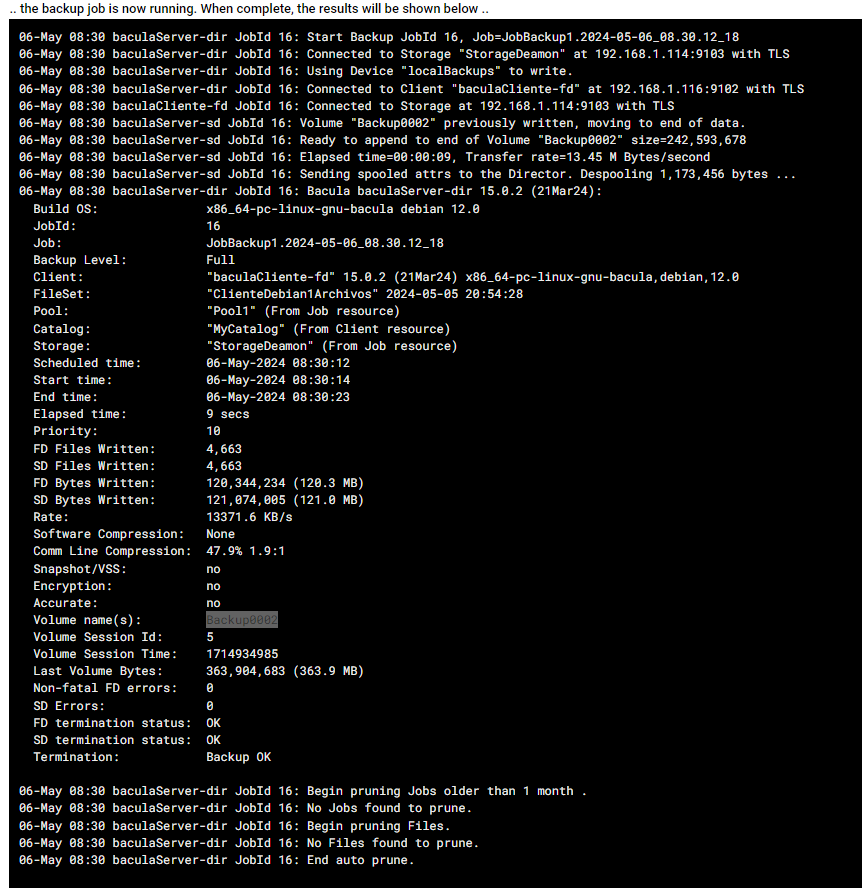
\includegraphics[width=0.5\linewidth]{instalacionBacula/backup0002.png}
    \caption{Realizando el respaldo de los archivos en Bacula.}
\end{figure}

Luego, eliminamos los archivos \texttt{archivo2.txt} y \texttt{archivo3.txt}:
\begin{figure}[H]
    \centering
    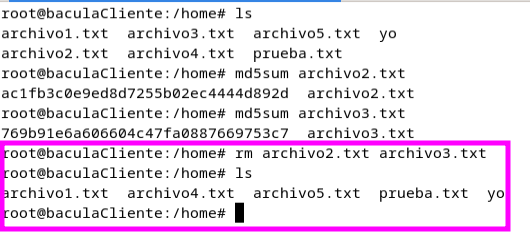
\includegraphics[width=0.5\linewidth]{instalacionBacula/rmArchivo23.png}
    \caption{Eliminación de los archivos que serán restaurados.}
\end{figure}

Procedemos con la restauración de los archivos eliminados:
\begin{figure}[H]
    \centering
    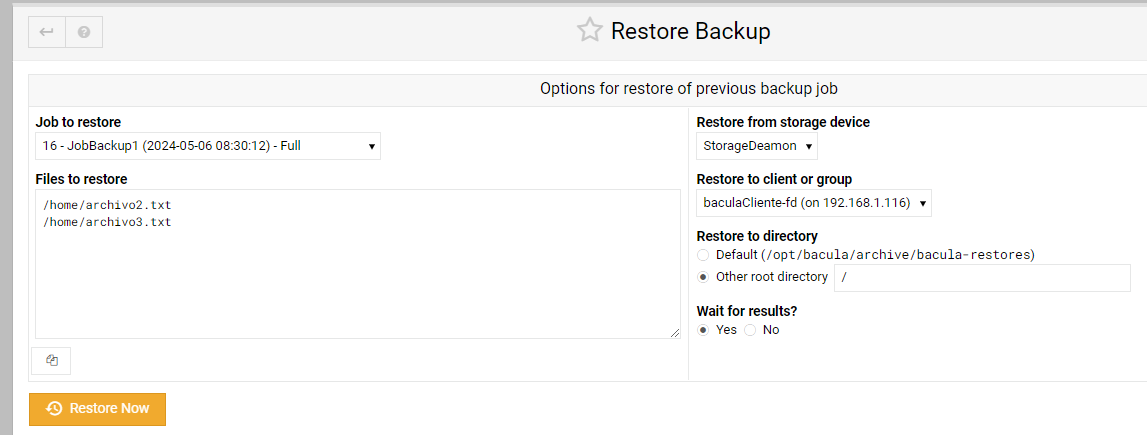
\includegraphics[width=0.5\linewidth]{instalacionBacula/resBackup.png}
    \caption{Configuración del proceso de restauración en Bacula.}
\end{figure}

Opciones para la restauración:
\begin{itemize}
    \item \textbf{Files to restore}: \texttt{/home/archivo2.txt}, \texttt{/home/archivo3.txt}
    \item \textbf{Restore from storage device}: \texttt{StorageDeamon}
    \item \textbf{Restore to client or group}: \texttt{baculaCliente-fd} (en 192.168.1.116)
    \item \textbf{Restore to directory}: opción por defecto (\texttt{/opt/bacula/archive/bacula-restores}) o directorio raíz (\texttt{/})
    \item \textbf{Wait for results}: Sí
\end{itemize}

\begin{figure}[H]
    \centering
    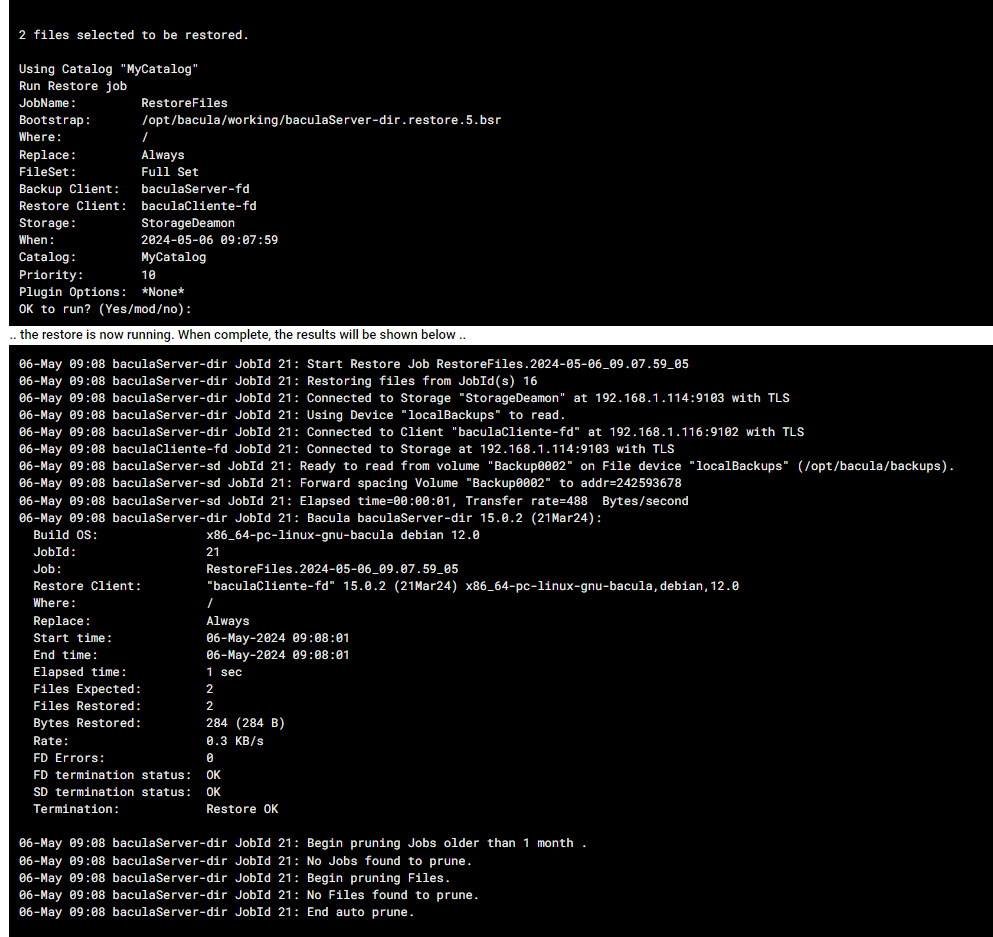
\includegraphics[width=0.5\linewidth]{instalacionBacula/restoresalidawebmin.png}
    \caption{salida de la restauración.}
\end{figure}

Una vez completada la restauración, confirmamos que los archivos han sido correctamente restaurados y verificamos su integridad:
\begin{figure}[H]
    \centering
    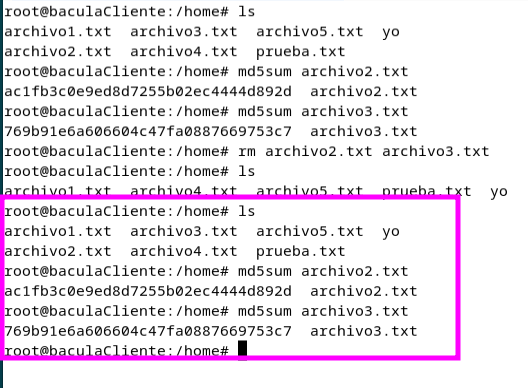
\includegraphics[width=0.5\linewidth]{instalacionBacula/restoreSusc.png}
    \caption{Verificación de los archivos restaurados en el cliente Linux.}
\end{figure}



\subsection{Backup y Restauración de Bases de Datos}

Para llevar a cabo un backup de una base de datos, inicialmente debemos definir un conjunto de archivos, conocido como \textit{fileset}. Aunque la interfaz de Webmin no permite crear un \textit{fileset} usando el plugin de Bacula pipe directamente, podemos hacerlo manualmente en el archivo de configuración \texttt{bacula-dir.conf}.

\begin{figure}[H]
    \centering
    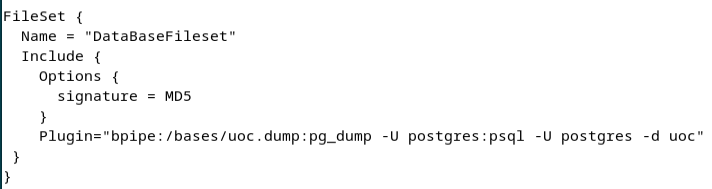
\includegraphics[width=0.5\linewidth]{instalacionBacula/filesetBpipe.png}
    \caption{Definición del FileSet para backups en Bacula.}
\end{figure}

Una vez definido el \textit{fileset}, procedemos a crear un nuevo trabajo de backup, especificando los detalles necesarios para su ejecución.

\textbf{Creación de un Trabajo de Backup}\medskip

Los detalles para la configuración del trabajo de backup son los siguientes:

\begin{itemize}
    \item \textbf{Nombre del trabajo:} DatabaseJOB
    \item \textbf{Habilitar trabajo:} Sí
    \item \textbf{Tipo por defecto:} Definición por defecto
    \item \textbf{Tipo de trabajo:} Backup
    \item \textbf{Nivel de backup:} Completo
    \item \textbf{Cliente a respaldar:} baculaCliente-fd
    \item \textbf{Conjunto de archivos a respaldar:} DataBaseFileset
    \item \textbf{Programación del backup:} Ciclo Semanal
    \item \textbf{Dispositivo de almacenamiento de destino:} StorageDaemon
    \item \textbf{Grupo de volúmenes:} Predeterminado
    \item \textbf{Destino de los mensajes:} Estándar
    \item \textbf{Prioridad del backup:} Predeterminada
\end{itemize}

\begin{figure}[H]
    \centering
    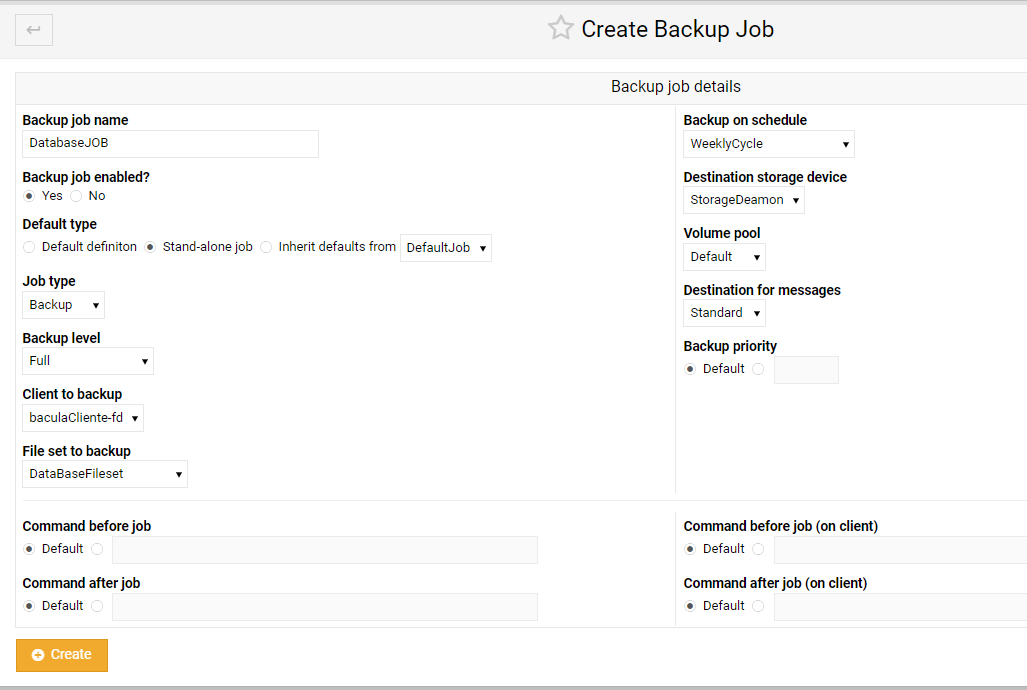
\includegraphics[width=0.5\linewidth]{instalacionBacula/databaseJOB.png}
    \caption{Detalles del trabajo de backup en Bacula.}
\end{figure}

\textbf{Eliminación de la Base de Datos}\medskip

A continuación, eliminamos la base de datos para simular una situación donde necesitemos restaurarla desde un backup:

\begin{figure}[H]
    \centering
    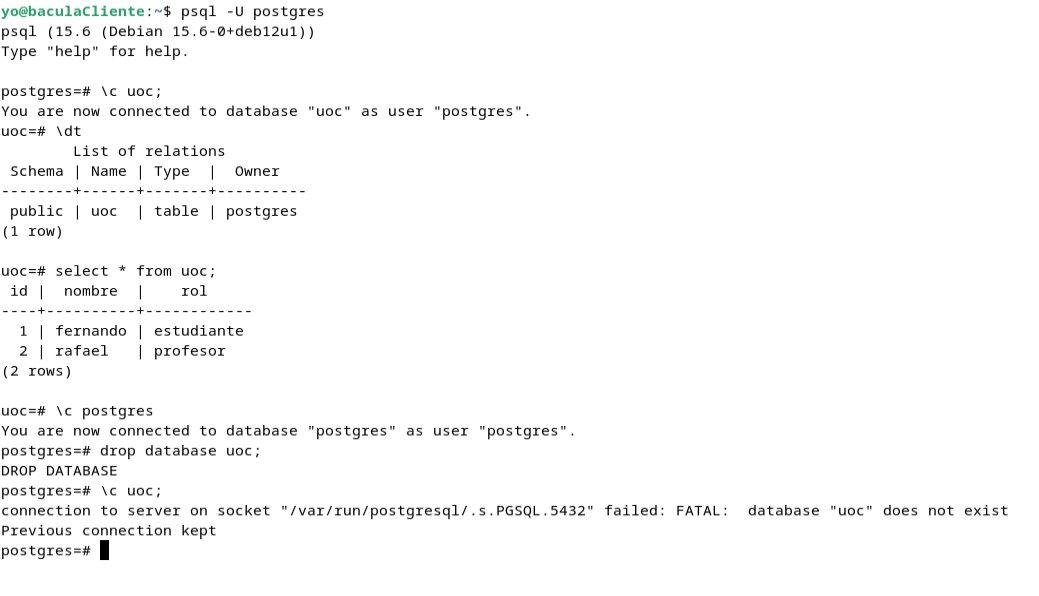
\includegraphics[width=0.5\linewidth]{instalacionBacula/dropdatabase.png}
    \caption{Comando para eliminar la base de datos \texttt{uoc}.}
\end{figure}

\textbf{Restauración de la Base de Datos}
\medskip

Realizamos la restauración de la base de datos y verificamos que las tablas sean restauradas correctamente:

\begin{figure}[H]
    \centering
    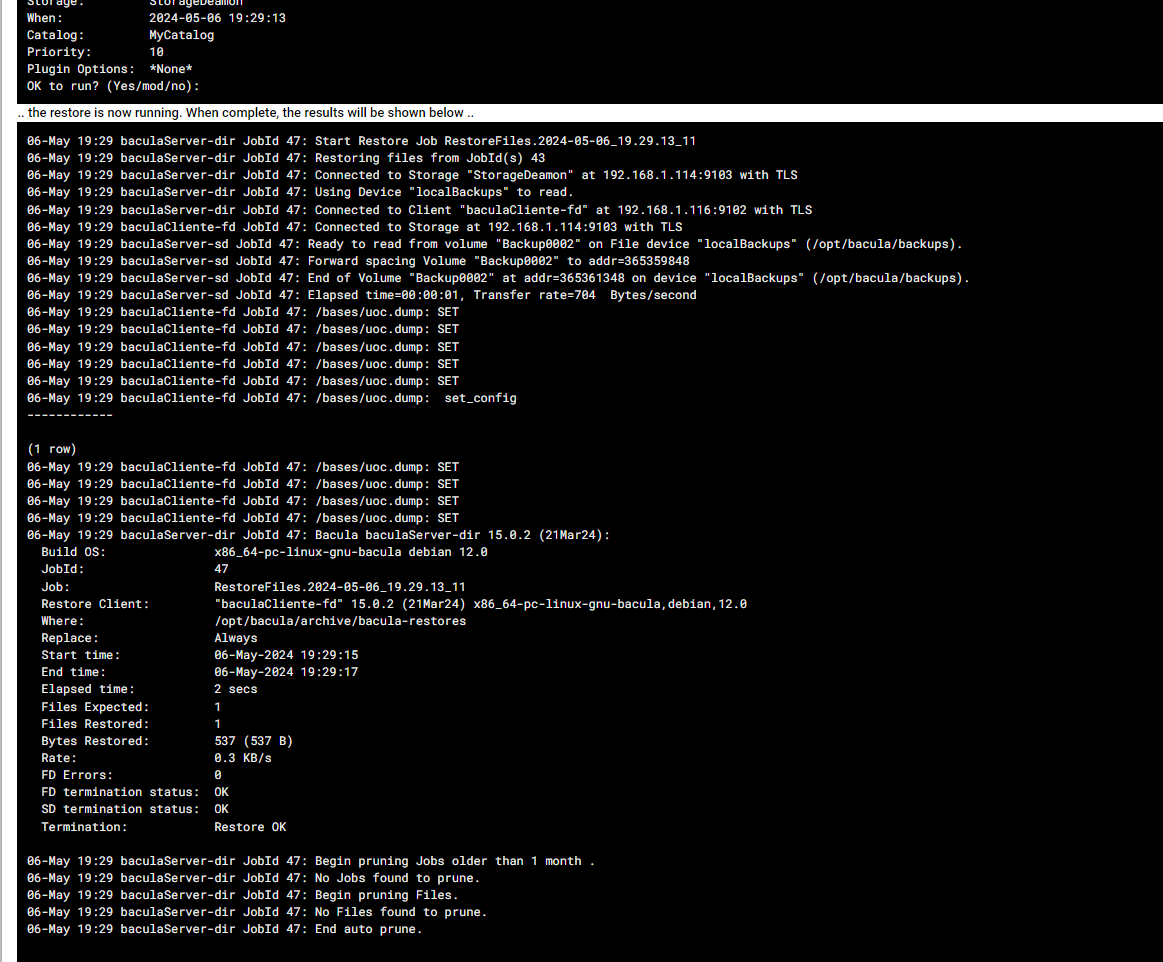
\includegraphics[width=0.5\linewidth]{instalacionBacula/restoreUOCdump.png}
    \caption{Proceso de restauración de la base de datos \texttt{uoc}.}
\end{figure}

Al finalizar la restauración, podemos confirmar que la tabla ha sido restaurada adecuadamente:

\begin{figure}[H]
    \centering
    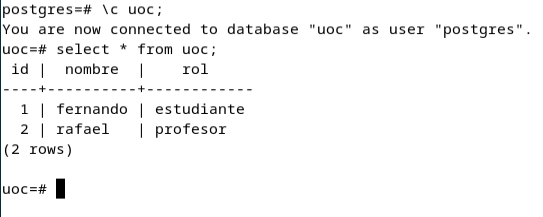
\includegraphics[width=0.5\linewidth]{instalacionBacula/restoreCompleteTABLAS.png}
    \caption{Tabla restaurada en la base de datos \texttt{uoc}.}
\end{figure}

\newpage


\section{DRP}

\subsection{Disaster Recovery Plan con Bacula}

Un \textbf{Disaster Recovery Plan} (DRP) es una estrategia documentada y detallada diseñada para proteger una organización contra la pérdida de datos y sistemas críticos en caso de un desastre. Este plan incluye procedimientos específicos para restaurar la infraestructura tecnológica y asegurar la rápida recuperación de la información esencial para mantener la continuidad del negocio.

La importancia de un DRP en la gestión de datos y sistemas no puede subestimarse. En el entorno actual, donde la información es uno de los activos más valiosos de una organización, cualquier tiempo de inactividad o pérdida de datos puede resultar en consecuencias financieras severas, pérdida de credibilidad y daño a la reputación a largo plazo. Un DRP efectivo asegura que la organización pueda recuperarse y reanudar las operaciones normales con el mínimo impacto posible.

Bacula, como una solución de software de backup y recuperación, juega un papel crucial en la implementación de un DRP. Ofrece herramientas robustas para la gestión de backups y la restauración de datos, permitiendo a las organizaciones enfrentar desastres con confianza y eficacia. A través de Bacula, las empresas pueden asegurarse de que todos los componentes críticos de su infraestructura tecnológica están protegidos y pueden ser restaurados rápidamente en caso necesario.

\subsection{Evaluación de Riesgos}

La evaluación de riesgos es un componente crítico de cualquier \textbf{Disaster Recovery Plan}. Este proceso implica la identificación y análisis de posibles riesgos que pueden amenazar los sistemas de información de una organización. El objetivo es entender la probabilidad de que estos eventos ocurran y el impacto potencial que podrían tener en la operatividad empresarial.

\subsubsection{Identificación de Riesgos}

Los riesgos pueden variar ampliamente dependiendo de varios factores, incluyendo la naturaleza del negocio, la ubicación geográfica, y la infraestructura tecnológica. Algunos de los riesgos más comunes incluyen:

\begin{itemize}
    \item Fallas de hardware o infraestructura, como servidores o dispositivos de almacenamiento que fallan.
    \item Ataques cibernéticos que pueden resultar en la pérdida o corrupción de datos.
    \item Desastres naturales que pueden causar daños físicos a los centros de datos y otros recursos críticos.
    \item Errores humanos que pueden llevar a la eliminación accidental de datos importantes.
\end{itemize}

\subsubsection{Análisis de Riesgos}

Una vez identificados los riesgos, es esencial evaluar su probabilidad y el impacto potencial. Esto se realiza mediante:

\begin{itemize}
    \item \textbf{Análisis de probabilidad}: Estimar la frecuencia con la que pueden ocurrir estos eventos.
    \item \textbf{Análisis de impacto}: Determinar el efecto potencial en la continuidad y recuperación del negocio. Este análisis ayuda a priorizar los riesgos y a planificar las respuestas apropiadas.
\end{itemize}

Bacula, como herramienta integral de backup y recuperación, es esencial en la mitigación de estos riesgos. Al proporcionar capacidades robustas de backup y restauración, Bacula asegura que, independientemente de la probabilidad o impacto de un desastre, los datos pueden ser recuperados de manera eficiente y efectiva, minimizando así la interrupción del negocio y protegiendo los activos de información.


\input{DRP/estrategiasDRP}
\subsection{Soluciones de Bacula para la Recuperación}

Bacula proporciona múltiples estrategias para asegurar la recuperación de datos en caso de pérdida del catálogo o de los propios datos. Estas estrategias permiten que la recuperación sea flexible y adaptable a diferentes escenarios de pérdida.

\subsubsection{Restauración del Catálogo mediante un Backup}

Bacula incluye automáticamente un job de backup del catálogo que es esencial para la recuperación rápida y eficiente del mismo en caso de pérdida. La restauración del catálogo desde un backup es el método más directo y efectivo para recuperar toda la información del estado de los backups anteriores.

\begin{itemize}
    \item \textbf{Proceso de Restauración}: Para restaurar el catálogo, se debe acceder al último backup del catálogo disponible y utilizar el comando adecuado para restaurar esta base de datos desde el archivo de backup.
    \item \textbf{Consideraciones}: Es crucial que los volúmenes donde están almacenados los backups del catálogo estén intactos y accesibles. Además, es importante mantener backups regulares del catálogo para minimizar la pérdida de datos de control.
\end{itemize}

\subsubsection{Restauración del Catálogo sin un Backup}

En situaciones donde no se dispone de un backup del catálogo, Bacula ofrece herramientas para reconstruir el catálogo examinando los volúmenes de backup.

\begin{itemize}
    \item \textbf{Métodos y Técnicas}:
        \begin{enumerate}
            \item \textbf{Restauración de la Base de Datos}: Si la base de datos se ha dañado, primero se debe reconstruir utilizando herramientas como \texttt{create\_bacula\_database}.
            \item \textbf{Reconstrucción del Catálogo}: Utilizar \texttt{bscan} para leer los volúmenes de backup y reconstruir el catálogo.
        \end{enumerate}
    \item \textbf{Escenarios}:
        \begin{enumerate}
            \item La base de datos está dañada y se necesita reconstruir antes de poder restaurar el catálogo.
            \item El backup del catálogo ha expirado su período de retención pero aún existen backups de datos en los volúmenes.
        \end{enumerate}
\end{itemize}

\subsubsection{Recuperación de Archivos Respaldados sin un Catálogo}

Existen casos en los que es necesario recuperar archivos directamente desde los medios de almacenamiento sin acceder al catálogo, por ejemplo, en un servidor diferente donde Bacula no está instalado.

\begin{itemize}
    \item \textbf{Proceso de Restauración}: Utilizar \texttt{bextract} para extraer archivos directamente desde los volúmenes de backup. Es necesario conocer la estructura aproximada del archivo de configuración \texttt{bacula-sd.conf} para realizar este proceso.
    \item \textbf{Consideraciones}: Este método requiere un conocimiento técnico más detallado de los formatos de almacenamiento y configuración de Bacula.
\end{itemize}





\section{Compresión}
\subsection{La Compresión en Bacula}

Bacula implementa una variedad de algoritmos de compresión para optimizar la eficiencia en la gestión de backups, permitiendo a los administradores reducir significativamente el espacio de almacenamiento requerido y el tiempo de transferencia de datos. Esto es especialmente útil en entornos con grandes volúmenes de datos o con limitaciones en la capacidad de almacenamiento.

\textbf{Tipos de Compresión Disponibles}\medskip

Bacula ofrece varios algoritmos de compresión que pueden ser seleccionados según las necesidades específicas del sistema de backup:

\begin{itemize}
    \item \textbf{GZIP}: utiliza varios niveles de compresión, desde el nivel 1, que es el más rápido y ofrece menos compresión, hasta el nivel 9, que es el más lento pero proporciona una compresión máxima.
    \item \textbf{LZO}: velocidad de compresión rápida con una eficacia de compresión razonable, equilibrando rendimiento y reducción de tamaño.
\end{itemize}

\textbf{Configuración de la Compresión por Defecto en Bacula}\medskip

Bacula utiliza un nivel de compresión por defecto cuando se configura el backup sin especificaciones explícitas. Este nivel predeterminado es el nivel 6 de GZIP. El nivel 6 ofrece un balance óptimo entre tiempo de compresión y reducción del tamaño de los datos, siendo adecuado para la mayoría de los entornos de backup. La selección de este nivel por defecto se basa en lograr un compromiso eficiente entre el tiempo de procesamiento y el ahorro de espacio.

\textbf{Consideraciones para la Elección del Nivel de Compresión}\medskip

Al configurar la compresión en Bacula, es importante considerar los siguientes factores:

\begin{itemize}
    \item \textbf{Naturaleza de los Datos}: Algunos tipos de datos, como imágenes y archivos de video ya comprimidos, pueden no beneficiarse mucho de la compresión adicional y podrían incluso aumentar de tamaño.
    \item \textbf{Recursos del Sistema}: La compresión consume CPU. En sistemas con recursos limitados, un nivel de compresión más bajo puede ser preferible.
    \item \textbf{Requerimientos de Rendimiento}: Sistemas con grandes volúmenes de datos o ventanas de backup cortas pueden requerir niveles de compresión más rápidos, como LZ4 o LZO.
\end{itemize}

La configuración flexible de Bacula permite a los administradores adaptar la compresión a las necesidades específicas del entorno, optimizando tanto el rendimiento como la utilización del espacio de almacenamiento.


\section{Velocidad de Backup y Restore }
\subsection{Concepto de la Velocidad de Backup y Restore}

La velocidad de backup se refiere al ritmo al que los datos son copiados durante un proceso de backup y restore, generalmente medido en megabytes por segundo (MB/s). Esta métrica es crucial para evaluar la eficiencia de las estrategias de backup implementadas en una organización. Una alta velocidad de backup asegura que grandes volúmenes de datos pueden ser respaldados en ventanas de tiempo reducidas, minimizando el impacto en las operaciones normales del sistema y reduciendo el tiempo durante el cual los datos están en riesgo de pérdida en caso de un fallo del sistema o desastre.

\subsubsection{Importancia de la Velocidad}

La velocidad a la que se pueden realizar los backups tiene un impacto directo en la gestión de copias de seguridad por varias razones:
\begin{itemize}
    \item \textbf{Eficiencia Operativa}: Trabajos rápidos significan menos tiempo de inactividad o degradación del rendimiento para los sistemas en uso. Esto es vital para entornos donde la disponibilidad continua es crítica, como en bases de datos en línea o sistemas transaccionales.
    \item \textbf{Cumplimiento de Ventanas de Backup}: Muchas organizaciones tienen períodos específicos en los que los trabajos deben completarse. Una mayor velocidad permite cumplir con estas ventanas sin comprometer la integridad del proceso de backup.
    \item \textbf{Reducción de Costes}: Menor tiempo de backup y restore implica menos uso de recursos dedicados, como la energía y el tiempo de operación del personal, lo cual puede traducirse en ahorros significativos a largo plazo.
\end{itemize}

\subsubsection{Impacto en la Operatividad y Recuperación ante Desastres}

Un sistema de eficiente y rápido no solo optimiza las operaciones diarias, sino que también juega un papel fundamental en la recuperación ante desastres:
\begin{itemize}
    \item \textbf{Disponibilidad de Datos}: En situaciones de desastre, la capacidad de restaurar datos rápidamente es crucial. Backups más rápidos facilitan backups más frecuentes, lo que reduce la cantidad de datos potencialmente perdidos entre cada backup.
    \item \textbf{Minimización de la Pérdida de Datos}: Con backups más frecuentes y rápidos, la ventana durante la cual los datos están expuestos a pérdidas se reduce significativamente.
    \item \textbf{Resiliencia Organizacional}: La capacidad de una organización para reanudar operaciones normales rápidamente después de un desastre depende en gran medida de su capacidad para restaurar información crítica desde sus backups eficientemente.
\end{itemize}


\subsubsection{Diferencias entre Velocidad de Backup y Velocidad de Restore}

Aunque tanto la velocidad de backup como la de restore son fundamentales para la gestión de la protección de datos, sus prioridades operacionales y técnicas difieren significativamente:

\begin{itemize}
    \item \textbf{Prioridades Operacionales}: Mientras que la velocidad de backup se centra en capturar y asegurar los datos de manera eficiente con el mínimo impacto en la operatividad diaria, la velocidad de restore se prioriza según la necesidad de accesibilidad y disponibilidad inmediata de los datos críticos para la recuperación y continuidad del negocio.
    \item \textbf{Aspectos Técnicos}: Los backups pueden ser programados para ejecutarse durante periodos de baja demanda para minimizar el impacto sobre el rendimiento del sistema, utilizando técnicas como la compresión y la deduplicación para optimizar el espacio y el tiempo. En contraste, la restauración debe ser capaz de descomprimir y ordenar esos datos eficientemente, a menudo bajo condiciones de tiempo crítico, y puede requerir un acceso más rápido y directo a los medios de almacenamiento.
\end{itemize}

Comprender estas diferencias es esencial para diseñar e implementar estrategias de backup y restore que no solo protejan los datos, sino que también garanticen que sean accesibles y utilizables tan pronto como sea necesario tras un incidente.

\subsection{Factores que Afectan la Velocidad en Bacula}

La velocidad de backup puede variar significativamente dependiendo de varios factores. Al comprender estos factores, los administradores pueden optimizar sus entornos para maximizar la eficiencia de los backups. En el contexto de Bacula, estos factores incluyen la configuración del hardware, el tamaño y tipo de datos, la configuración del software de backup y la gestión de la concurrencia.

\subsubsection{Influencia del Hardware}

El hardware juega un papel crucial en la velocidad. Los componentes clave a considerar incluyen:

\begin{itemize}
    \item \textbf{Velocidad del Procesador}: Un procesador más rápido puede manejar las compresiones y cifrados de datos con mayor eficacia, acelerando el proceso de backup.
    \item \textbf{Cantidad de Memoria RAM}: Suficiente RAM es esencial para manejar grandes volúmenes de datos y operaciones simultáneas sin recurrir a la memoria swap, que es considerablemente más lenta.
    \item \textbf{Tipo y Velocidad de los Discos Duros}: Los discos SSD, por ejemplo, ofrecen tiempos de acceso y escritura más rápidos que los discos duros tradicionales, lo cual puede reducir significativamente el tiempo de backup y restore.
    \item \textbf{Infraestructura de Red}: La velocidad de la red afecta directamente la velocidad que involucran transferencia de datos a través de la red. Redes más rápidas permiten transferencias más rápidas de los datos a respaldar.
\end{itemize}

\subsubsection{Tamaño y Tipo de Datos}

El volumen y la naturaleza de los datos son también factores determinantes en la velocidad:

\begin{itemize}
    \item \textbf{Volumen de Datos}: Mayores cantidades de datos generalmente requieren más tiempo para ser respaldados.
    \item \textbf{Tipo de Archivos}: Datos como imágenes y videos que ya están comprimidos no se beneficiarán tanto de la compresión adicional y pueden tomar más tiempo en procesarse.
    \item \textbf{Compresión y Deduplicación}: Estas tecnologías pueden reducir significativamente el volumen de datos a transferir, aunque el proceso de deduplicación y compresión en sí mismo también consume recursos y tiempo.
\end{itemize}

\subsubsection{Software de Backup y Configuración}

La configuración del software, como Bacula, tiene un impacto directo en la velocidad de backup. Bacula ofrece opciones avanzadas que pueden ser ajustadas para mejorar la velocidad:

\begin{itemize}
    \item \textbf{Nivel de Compresión}: Ajustar el nivel de compresión puede equilibrar la carga de trabajo del procesador y la cantidad de datos a escribir.
    \item \textbf{Configuraciones de Network Buffering}: Optimizar estos parámetros puede mejorar el rendimiento de las transferencias de datos a través de la red.
    \item \textbf{Directivas de Backup}: La selección de directivas adecuadas puede minimizar la cantidad de datos que necesitan ser respaldados, al excluir archivos innecesarios o temporales.
\end{itemize}

\subsubsection{Concurrencia y Multitasking}

La habilidad para realizar múltiples operaciones de backup simultáneamente es esencial para entornos grandes:

\begin{itemize}
    \item \textbf{Gestión de Tareas Simultáneas}: Bacula permite configurar múltiples jobs de backup y restore en paralelo, lo que puede mejorar la utilización de los recursos pero también puede competir por el ancho de banda de red y otros recursos.
    \item \textbf{Planificación Inteligente}: Organizar los jobs de backup para que se ejecuten en momentos de baja demanda puede evitar la saturación de la red y de los recursos del servidor, manteniendo una alta velocidad de backup.
\end{itemize}


\subsection{Medición de la Velocidad en Bacula}

La medición precisa de la velocidad de backup es esencial para garantizar la eficiencia y la efectividad de cualquier sistema de gestión de backups. En el caso de Bacula, existen varias metodologías y herramientas que pueden ser utilizadas para evaluar esta métrica crítica.

\subsubsection{Metodologías y Herramientas para la Medición}

Para medir la velocidad de backup efectiva en Bacula, se pueden considerar los siguientes enfoques y herramientas:

\begin{itemize}
    \item \textbf{Registro de Logs}: Bacula genera logs detallados que incluyen información sobre la duración de cada job de backup, el tamaño total de los datos procesados y la velocidad de transferencia de datos. Estos logs pueden ser analizados para obtener métricas de rendimiento precisas.
    \item \textbf{Bacula's Status Command}: Este comando permite a los administradores obtener información en tiempo real sobre el estado de los jobs de backup en curso, incluyendo la velocidad actual de backup.
    \item \textbf{Herramientas Externas}: Herramientas de monitoreo de red y rendimiento del sistema, como Nagios, Zabbix o Grafana, pueden integrarse con Bacula para proporcionar visualizaciones en tiempo real y alertas basadas en el rendimiento de los backups.
    \item \textbf{Pruebas de Benchmarking}: Realizar pruebas de rendimiento controladas utilizando herramientas específicas de benchmarking que simulan diferentes escenarios de carga de trabajo para evaluar la capacidad del sistema de backups.
\end{itemize}

\subsubsection{Importancia de las Pruebas Regulares}

Realizar pruebas regulares de velocidad de backup es vital por varias razones:

\begin{itemize}
    \item \textbf{Validación de la Configuración}: Las pruebas ayudan a confirmar que la configuración del sistema de backups está optimizada para la infraestructura actual.
    \item \textbf{Identificación de Cuellos de Botella}: Las pruebas regulares permiten identificar y resolver cuellos de botella en la red, en el almacenamiento o en el procesamiento, que podrían estar limitando la velocidad de backup.
    \item \textbf{Adaptación a Cambios}: En entornos dinámicos, donde las cargas de trabajo y los volúmenes de datos pueden cambiar frecuentemente, las pruebas regulares aseguran que los backups sigan siendo eficientes y efectivos.
    \item \textbf{Cumplimiento de SLAs}: Asegura que los tiempos de backup cumplen con los Acuerdos de Nivel de Servicio establecidos, evitando posibles penalizaciones o problemas de cumplimiento.
\end{itemize}

Medir y probar la velocidad de backup y restore de manera regular en Bacula no solo garantiza que los datos estén protegidos de manera eficiente, sino que también proporciona la confianza de que el sistema de backups puede recuperar esos datos en un tiempo aceptable en caso de una falla o desastre.


\subsection{Estrategias para Mejorar la Velocidad de Backup y Restore en Bacula}

Optimizar la velocidad de Backup y Restore es crucial para minimizar el tiempo de inactividad y maximizar la eficiencia operativa. En Bacula, existen diversas estrategias que se pueden implementar para mejorar este aspecto, desde la optimización del hardware hasta ajustes avanzados en el software y la infraestructura de TI.

\subsubsection{Optimización del Hardware}

Mejorar el hardware puede tener un impacto significativo en la velocidad de Backup y Restore. Las siguientes son algunas sugerencias:

\begin{itemize}
    \item \textbf{Actualizar el Almacenamiento}: Utilizar SSDs en lugar de discos duros tradicionales para reducir el tiempo de acceso y mejorar las tasas de transferencia de datos.
    \item \textbf{Mejorar la Red}: Implementar redes de mayor velocidad y configurar adecuadamente los adaptadores de red para soportar mayores cargas de tráfico.
    \item \textbf{Incrementar la RAM}: Aumentar la memoria RAM para facilitar el procesamiento rápido de los datos durante las operaciones y reducir el uso de swap.
    \item \textbf{Procesadores más rápidos}: Invertir en CPUs más potentes para manejar de manera más eficiente las operaciones de compresión y cifrado.
\end{itemize}

\subsubsection{Ajustes en el Software}

Bacula ofrece varias configuraciones que pueden ajustarse para mejorar la velocidad:

\begin{itemize}
    \item \textbf{Compresión y Deduplicación}: Ajustar los niveles de compresión y habilitar la deduplicación para reducir la cantidad de datos que necesitan ser transferidos y almacenados.
    \item \textbf{Priorización de Tareas}: Configurar la prioridad de los jobs de backup para optimizar el rendimiento durante los períodos de alta demanda.
    \item \textbf{Configuración de Buffers de Red}: Optimizar los buffers de red en Bacula para mejorar la eficiencia de las transferencias de datos a través de la red.
\end{itemize}

\subsubsection{Planificación Inteligente }

La programación de backups durante períodos de bajo uso es fundamental para no impactar negativamente en el rendimiento del sistema:

\begin{itemize}
    \item \textbf{Horarios de Bajo Tráfico}: Programar backups para horas nocturnas o durante fines de semana cuando la utilización de la red y del sistema es mínima.
    \item \textbf{Frecuencia de Backups}: Ajustar la frecuencia de los backups según la criticidad de los datos, permitiendo flexibilidad y minimizando la carga en la infraestructura.
\end{itemize}

\subsubsection{Tecnologías Avanzadas}

Implementar tecnologías avanzadas puede ofrecer mejoras sustanciales en la velocidad de backups:

\begin{itemize}
    \item \textbf{Almacenamiento en Caché}: Utilizar sistemas de caché para almacenar temporalmente los datos antes de transferirlos al sistema de almacenamiento de backups, reduciendo así el tiempo de backup.
    \item \textbf{Uso de SSDs}: Implementar SSDs para almacenamiento de datos de backup puede significativamente aumentar la velocidad debido a su rápida capacidad de escritura y lectura.
\end{itemize}



%\section{Velocidad de restore}
%\subsection{Concepto la Velocidad de Restore}

La velocidad de restore se refiere al tiempo que se tarda en recuperar datos desde un medio de backup hasta que están completamente disponibles para su uso después de un evento disruptivo o durante operaciones de mantenimiento rutinarias. Esta métrica es crucial para la continuidad del negocio y la gestión de desastres, ya que determina la capacidad de una organización para volver a la normalidad operativa tras una interrupción.

\subsubsection{Importancia de la Velocidad de Restore}

La velocidad con la que los datos pueden ser restaurados afecta directamente el Tiempo de Inactividad Tolerable (TIT) y los Objetivos de Tiempo de Recuperación (RTO) de una empresa. Un RTO bajo es esencial para aplicaciones críticas donde incluso una pequeña cantidad de tiempo de inactividad puede resultar en pérdidas significativas o en riesgos de seguridad. En contextos de desastre, una restauración rápida es vital para minimizar el impacto financiero y operativo, asegurando que los servicios esenciales puedan ser reanudados rápidamente.

\subsubsection{Diferencias entre Velocidad de Backup y Velocidad de Restore}

Aunque tanto la velocidad de backup como la de restore son fundamentales para la gestión de la protección de datos, sus prioridades operacionales y técnicas difieren significativamente:

\begin{itemize}
    \item \textbf{Prioridades Operacionales}: Mientras que la velocidad de backup se centra en capturar y asegurar los datos de manera eficiente con el mínimo impacto en la operatividad diaria, la velocidad de restore se prioriza según la necesidad de accesibilidad y disponibilidad inmediata de los datos críticos para la recuperación y continuidad del negocio.
    \item \textbf{Aspectos Técnicos}: Los backups pueden ser programados para ejecutarse durante periodos de baja demanda para minimizar el impacto sobre el rendimiento del sistema, utilizando técnicas como la compresión y la deduplicación para optimizar el espacio y el tiempo. En contraste, la restauración debe ser capaz de descomprimir y ordenar esos datos eficientemente, a menudo bajo condiciones de tiempo crítico, y puede requerir un acceso más rápido y directo a los medios de almacenamiento.
\end{itemize}

Comprender estas diferencias es esencial para diseñar e implementar estrategias de backup y restore que no solo protejan los datos, sino que también garanticen que sean accesibles y utilizables tan pronto como sea necesario tras un incidente.

%\subsection{Factores que Afectan la Velocidad de Restore}

Diversos factores influyen en la velocidad con la que los datos pueden ser restaurados en un sistema gestionado por Bacula. A continuación, se destacan algunos de los principales elementos que impactan esta velocidad, muchos de los cuales son comunes también a la velocidad de backup.

\textbf{Tipo de Medio de Almacenamiento}

El tipo de almacenamiento utilizado para los backups juega un papel crucial en los tiempos de restore. Los discos de estado sólido (SSD) permiten un acceso más rápido a los datos en comparación con los discos duros tradicionales (HDD) y las cintas. Mientras que los SSDs ofrecen tiempos de acceso casi instantáneos, las cintas pueden requerir más tiempo debido a su naturaleza secuencial.

\textbf{Localización de los Datos}

La ubicación física o geográfica de los datos almacenados también afecta la velocidad de restore. Los datos almacenados localmente (on-site) generalmente se recuperan más rápidamente que aquellos almacenados en ubicaciones remotas (off-site) o en la nube, debido a las limitaciones inherentes de la transferencia de datos a través de la red.

\textbf{Integridad y Formato de los Datos}

La integridad y el formato de los archivos son cruciales para los tiempos de restauración. Los archivos que están comprimidos o encriptados pueden requerir procesos adicionales para su descompresión y descifrado, lo que puede prolongar significativamente el tiempo de restore.

\textbf{Configuración del Software de Backup}

Finalmente, las configuraciones específicas en Bacula, como la deduplicación inversa, influyen directamente en la eficiencia de los restores. Ajustar estas configuraciones puede optimizar el tiempo necesario para recuperar los datos, aunque es necesario un balance entre la eficiencia durante el backup y la velocidad durante el restore.

%\subsection{Medición de la Velocidad de Restore en Bacula}

La capacidad para restaurar datos rápidamente es crucial para minimizar el impacto operativo tras un fallo o desastre. La medición efectiva de la velocidad de restore es fundamental para garantizar que los sistemas de recuperación funcionan dentro de los parámetros aceptables y cumplen con los Objetivos de Tiempo de Recuperación (RTO) establecidos por la organización.

\subsubsection{Metodologías y Herramientas para Medir la Velocidad de Restore}

Para medir la velocidad de restore en Bacula, se pueden emplear varias metodologías y herramientas:

\begin{itemize}
    \item \textbf{Pruebas de Recuperación}: Realizar simulacros de desastre y pruebas de restauración planificadas permite evaluar cuánto tiempo toma recuperar datos en diferentes escenarios. Esto ayuda a identificar posibles cuellos de botella y a ajustar configuraciones para optimizar la velocidad de restore.
    \item \textbf{Monitoreo en Tiempo Real}: Utilizar herramientas de monitoreo en tiempo real para rastrear la velocidad de las operaciones de restore mientras ocurren. Herramientas como Nagios, Zabbix o herramientas integradas de Bacula pueden proporcionar alertas instantáneas si el rendimiento cae por debajo de un umbral aceptable.
    \item \textbf{Registro y Análisis de Logs}: Bacula guarda registros detallados de cada operación de restore, que pueden ser analizados posteriormente para evaluar la eficiencia y la velocidad de las restauraciones completadas.
\end{itemize}

\subsubsection{Importancia de las Pruebas Regulares}

Realizar pruebas regulares de restore es esencial por varias razones:

\begin{itemize}
    \item \textbf{Verificación de RTO}: Las pruebas ayudan a asegurar que los RTOs, que son parte crítica de los Acuerdos de Nivel de Servicio (SLAs), se cumplan consistentemente, protegiendo así la capacidad de la empresa para recuperarse de interrupciones.
    \item \textbf{Optimización Continua}: Permite a los administradores ajustar y optimizar la configuración de Bacula y la infraestructura subyacente para mejorar continuamente los tiempos de restore.
    \item \textbf{Preparación para Desastres}: Las pruebas regulares aumentan la preparación para desastres, asegurando que tanto el personal como los sistemas están listos para ejecutar procedimientos de recuperación bajo presión.
\end{itemize}



%\subsection{Estrategias para Mejorar la Velocidad de Restore en Bacula}

Una recuperación rápida y eficiente de los datos es fundamental para minimizar el tiempo de inactividad y mantener la continuidad del negocio. En Bacula, existen varias estrategias que pueden implementarse para mejorar la velocidad de restore, desde la optimización del hardware hasta la configuración avanzada del software.

\subsubsection{Optimización de Hardware y Red}

El hardware y la infraestructura de red juegan un papel crucial en los tiempos de recuperación de datos. Mejorar estos aspectos puede resultar en una significativa reducción en el tiempo de restore:

\begin{itemize}
    \item \textbf{Mejora de los Medios de Almacenamiento}: Utilizar discos SSD en lugar de HDD tradicionales para el almacenamiento de los backups puede mejorar la velocidad de acceso a los datos durante las operaciones de restore.
    \item \textbf{Redes de Alta Velocidad}: Implementar redes más rápidas y más eficientes, como Gigabit Ethernet o incluso redes de 10 Gigabit, para asegurar que la transferencia de datos desde y hacia el servidor de Bacula sea lo más rápida posible.
\end{itemize}

\subsubsection{Ajustes en el Software de Backup}

Configurar adecuadamente el software de backup Bacula puede tener un impacto significativo en la velocidad de restore:

\begin{itemize}
    \item \textbf{Tamaño del Bloque}: Ajustar el tamaño del bloque en la configuración de Bacula puede ayudar a optimizar la lectura de datos desde el medio de almacenamiento, reduciendo así el tiempo total de restauración.
    \item \textbf{Paralelización de Tareas de Restore}: Habilitar la ejecución paralela de tareas de restore puede disminuir significativamente el tiempo de recuperación, especialmente en entornos con múltiples máquinas que necesitan ser restauradas simultáneamente.
\end{itemize}

\subsubsection{Planificación Inteligente de Restores}

La planificación estratégica de las operaciones de restore puede mejorar en gran medida la eficiencia de todo el proceso:

\begin{itemize}
    \item \textbf{Priorización de Restores}: Determinar qué datos son más críticos y deben ser restaurados primero puede reducir el impacto operativo de un desastre, asegurando que los servicios esenciales sean rápidamente restablecidos.
    \item \textbf{Restores Programados Durante Horas de Bajo Uso}: Planificar restores durante periodos de menor actividad puede maximizar los recursos disponibles y minimizar la interferencia con las operaciones normales de la empresa.
\end{itemize}



\section{Resultados}


\subsection{Resultados de la Velocidad de Backup en Diferentes Tamaños de Archivos}

En este apartado se presentan los resultados obtenidos al medir la velocidad de backup para diferentes tamaños de archivos. La Figura \ref{fig:backup-velocidad-tamaño} muestra los tiempos de backup en función del tamaño del archivo.

\begin{figure}[H]
    \centering
    \includegraphics[width=0.8\textwidth]{backup_velocidad_tamaño.png}
    \caption{Velocidades de Backup para Diferentes Tamaños de Archivo}
    \label{fig:backup-velocidad-tamaño}
\end{figure}

\textbf{Descripción de los Datos:}
Los datos muestran que para archivos de hasta 100 MB, el tiempo de backup es prácticamente constante y muy bajo (menos de un segundo). Sin embargo, a medida que el tamaño del archivo aumenta a 1 GB y más, el tiempo de backup incrementa de manera significativa. Para archivos de 10 GB, el tiempo de backup llega a superar los 450 segundos.

\textbf{Análisis de Resultados:}
Los resultados indican una relación no lineal entre el tamaño del archivo y el tiempo de backup, observándose un crecimiento exponencial del tiempo de backup a medida que el tamaño del archivo aumenta. Este comportamiento sugiere que para tamaños de archivo pequeños, la sobrecarga inicial del sistema y la latencia no afectan significativamente el tiempo de backup. Sin embargo, para archivos más grandes, la cantidad de datos que se debe procesar y transferir domina el tiempo total de backup. Este crecimiento exponencial es esperable, dado que a medida que aumenta el tamaño del archivo, se incrementa también la cantidad de operaciones de entrada y salida, así como la carga de procesamiento requerida para manejar los datos.

\textbf{Incertidumbre de la Medida:}
También es importante destacar que la incertidumbre o el error en la medición del tiempo de backup crece con el tamaño del archivo. Esto se puede observar en las barras de error presentes en la gráfica, las cuales se vuelven más pronunciadas a medida que aumenta el tamaño del archivo. Esta creciente incertidumbre refleja las variaciones y posibles fluctuaciones en el rendimiento del sistema durante el proceso de backup, especialmente para archivos de gran tamaño.

\textbf{Importancia del Tamaño del Pool:}
El tamaño del pool de almacenamiento es un factor crítico en la eficiencia del backup. Un pool más grande puede manejar archivos grandes más eficientemente al distribuir la carga de trabajo entre más recursos. Sin embargo, si el pool es demasiado pequeño, puede convertirse en un cuello de botella, incrementando significativamente los tiempos de backup. Por lo tanto, es crucial dimensionar adecuadamente el pool de almacenamiento para asegurar una operación de backup eficiente y escalable.




%%%%%%%%%%%%%%%%%%%%%%%%%%%%%%%%%%%%%%%%%%%%%%%%%
\subsection{Resultados de la Velocidad de Backup de 1 GB en Diferentes Tamaños de Archivos de Fracción de 1 GB}

En este apartado se presentan los resultados obtenidos al medir la velocidad de backup para un archivo de 1 GB, dividido en diferentes tamaños de archivos más pequeños. La Figura \ref{fig:backup-velocidad1gb} muestra los tiempos de backup en función del tamaño de la fracción de archivo.

\begin{figure}[H]
    \centering
    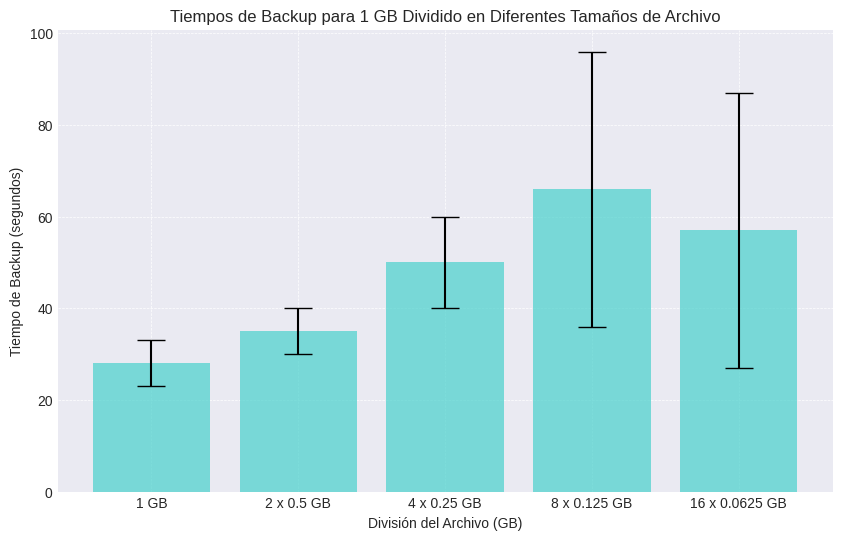
\includegraphics[width=0.8\textwidth]{backup_velocidad1gb.png}
    \caption{Tiempos de Backup para 1 GB Dividido en Diferentes Tamaños de Archivo}
    \label{fig:backup-velocidad1gb}
\end{figure}

\textbf{Descripción de los Datos:}
Los datos muestran que al dividir un archivo de 1 GB en fracciones más pequeñas, el tiempo de backup varía significativamente. Para un solo archivo de 1 GB, el tiempo de backup es de aproximadamente 28 segundos con una desviación estándar de ±5 segundos. Cuando se divide en dos archivos de 0.5 GB, el tiempo de backup aumenta a aproximadamente 35 segundos con una desviación estándar de ±5 segundos. Al dividirse en cuatro archivos de 0.25 GB, el tiempo de backup sube a unos 50 segundos con una desviación estándar de ±10 segundos. La división en ocho archivos de 0.125 GB resulta en un tiempo de backup de aproximadamente 66 segundos con una desviación estándar de ±30 segundos. Finalmente, la división en dieciséis archivos de 0.0625 GB muestra un tiempo de backup de unos 57 segundos con una desviación estándar de ±30 segundos.

\textbf{Análisis de Resultados:}
Los resultados indican que el tiempo de backup no aumenta linealmente con la división del archivo de 1 GB en fracciones más pequeñas. En cambio, se observa un aumento inicial del tiempo de backup cuando se pasa de un único archivo a varias fracciones, seguido de una mayor variabilidad en los tiempos de backup a medida que el número de fracciones aumenta. Esta variabilidad es notable en las barras de error, que se vuelven más pronunciadas a medida que disminuye el tamaño de cada fracción.

\textbf{Comportamiento Observado:}
La tendencia observada puede deberse a varios factores, incluyendo la sobrecarga administrativa asociada con el manejo de múltiples archivos y la mayor cantidad de operaciones de entrada y salida requeridas para procesar estos archivos más pequeños. La creciente incertidumbre en las mediciones para tamaños de fracción más pequeños sugiere que otros factores del sistema, como la latencia y la carga de procesamiento, tienen un impacto más pronunciado cuando se manejan múltiples archivos simultáneamente.


%%%%%%%%%%%%%%%%%%%%%%%%%%%%%%%%%%%%%%%%%%%%%%%%

\subsection{Resultados del Impacto de los Niveles de Compresión en la Compresión, Velocidad y Bytes Escritos}

En este apartado se presentan los resultados obtenidos al medir cómo los diferentes niveles de compresión (LZO y GZIP del 1 al 9) afectan la compresión, la velocidad de respaldo y los bytes escritos. A continuación se presentan y discuten los resultados obtenidos.

\begin{figure}[H]
    \centering
    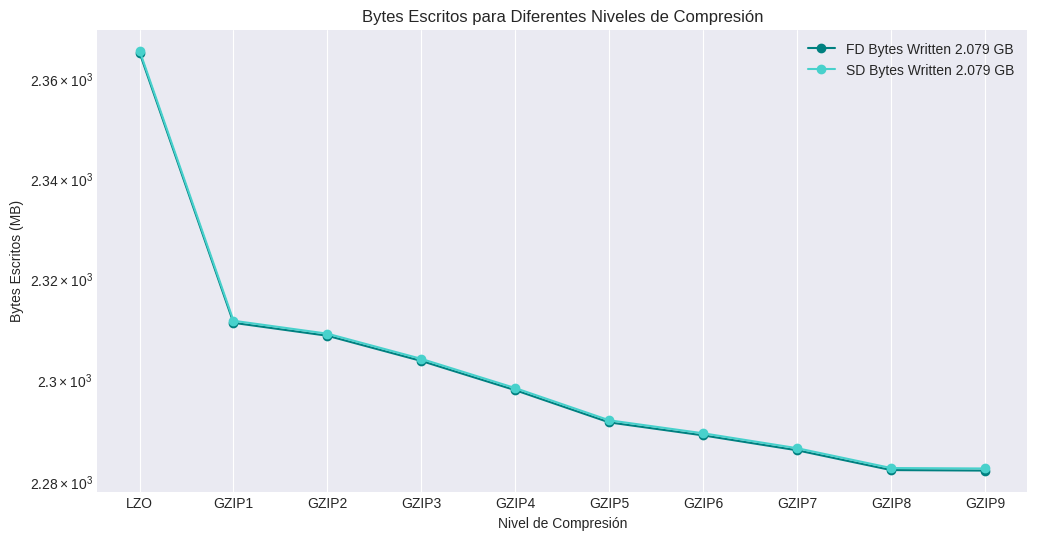
\includegraphics[width=0.8\textwidth]{bytes_escritos_archivo_grande.png}
    \caption{Bytes Escritos para Diferentes Niveles de Compresión (Archivo de 2.079 GB)}
    \label{fig:bytes_escritos_grande}
\end{figure}

\begin{figure}[H]
    \centering
    \includegraphics[width=0.8\textwidth]{bytes_escritos_archivo_pequeño.png}
    \caption{Bytes Escritos para Diferentes Niveles de Compresión (Archivo de 42 MB)}
    \label{fig:bytes_escritos_pequeño}
\end{figure}

\begin{figure}[H]
    \centering
    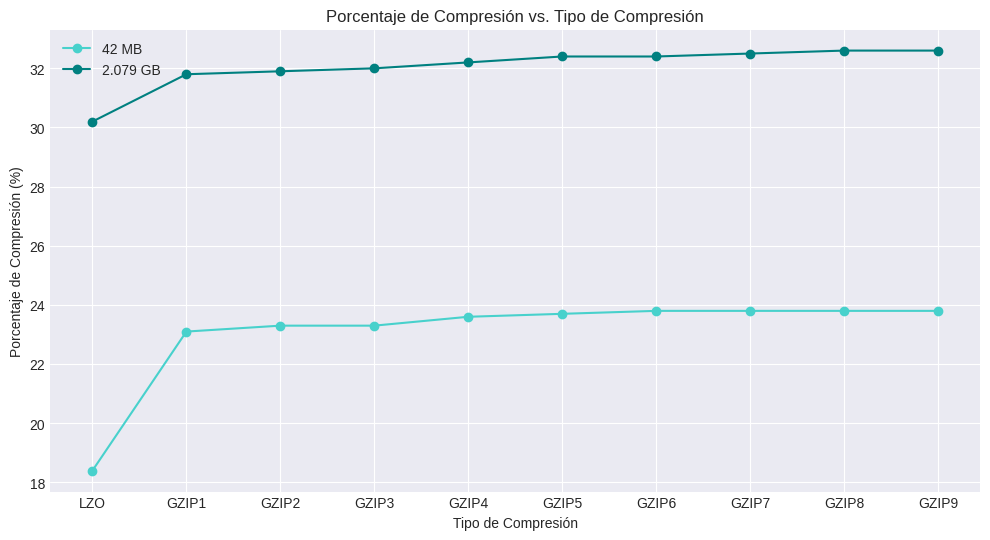
\includegraphics[width=0.8\textwidth]{porcentaje_compresion.png}
    \caption{Porcentaje de Compresión vs. Tipo de Compresión}
    \label{fig:porcentaje_compresion}
\end{figure}

\begin{figure}[H]
    \centering
    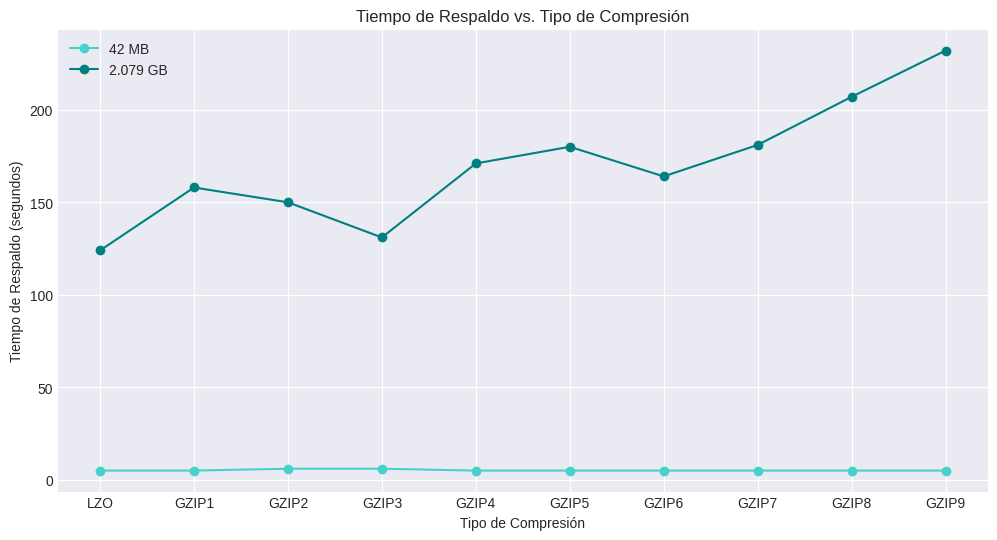
\includegraphics[width=0.8\textwidth]{tiempo_respaldo.png}
    \caption{Tiempo de Respaldo vs. Tipo de Compresión}
    \label{fig:tiempo_respaldo}
\end{figure}

\textbf{Bytes Escritos:}
La Figura \ref{fig:bytes_escritos_grande} y la Figura \ref{fig:bytes_escritos_pequeño} muestran los bytes escritos por el File Daemon (FD) y el Storage Daemon (SD) para un archivo de 2.079 GB y 42 MB, respectivamente, bajo diferentes niveles de compresión. Se observa que el uso de GZIP, incluso en su nivel más bajo (GZIP1), reduce significativamente la cantidad de bytes escritos en comparación con LZO. A medida que aumenta el nivel de compresión de GZIP, los bytes escritos continúan disminuyendo, aunque el decremento se vuelve menos pronunciado en los niveles más altos.

\textbf{Porcentaje de Compresión:}
La Figura \ref{fig:porcentaje_compresion} muestra el porcentaje de compresión alcanzado con LZO y diferentes niveles de GZIP para archivos de 42 MB y 2.079 GB. Los resultados indican que GZIP logra una mayor compresión que LZO. En particular, el porcentaje de compresión mejora ligeramente con niveles más altos de GZIP, aunque la diferencia se reduce a partir de GZIP6. Para los archivos más grandes, el porcentaje de compresión es consistentemente más alto en comparación con los archivos más pequeños.

\textbf{Tiempo de Respaldo:}
La Figura \ref{fig:tiempo_respaldo} presenta los tiempos de respaldo para los archivos de 42 MB y 2.079 GB bajo diferentes niveles de compresión. Se observa que el tiempo de respaldo aumenta con niveles más altos de compresión, especialmente para el archivo más grande. El tiempo de respaldo con LZO es significativamente menor que con GZIP, lo que sugiere que aunque GZIP proporciona una mejor compresión, lo hace a costa de un mayor tiempo de procesamiento.

\textbf{Análisis de Resultados:}
Los resultados muestran que la elección del algoritmo de compresión y su nivel tiene un impacto significativo en los bytes escritos, el porcentaje de compresión y el tiempo de respaldo. GZIP, especialmente en niveles más altos, ofrece una mayor compresión en comparación con LZO, pero con un incremento notable en el tiempo de respaldo. Esto sugiere que para optimizar la eficiencia de almacenamiento, GZIP es preferible, mientras que LZO puede ser más adecuado cuando el tiempo de respaldo es una consideración crítica.

%%%%%%%%%%%%%%%%%%%%%%%%%%%%%%%%%%%%%%%%%%%%%%%



\subsection{Resultados de los Tiempos de Restauración para los Distintos Tamaños de Archivos}

En este apartado se presentan los resultados obtenidos al medir los tiempos de restauración para diferentes tamaños de archivos. La Figura \ref{fig:tiempo-restauracion} muestra los tiempos de restauración en función del tamaño del archivo.

\begin{figure}[H]
    \centering
    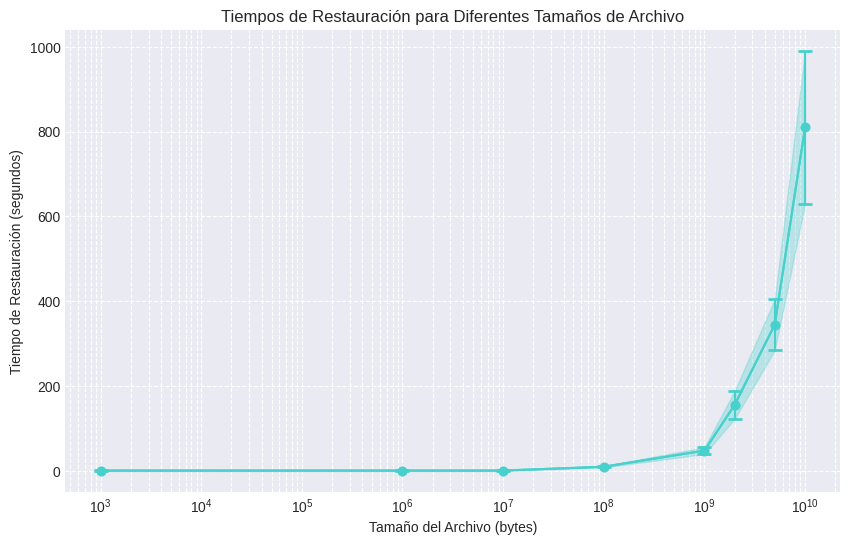
\includegraphics[width=0.8\textwidth]{tiempo_restauracion.png}
    \caption{Tiempos de Restauración para Diferentes Tamaños de Archivo}
    \label{fig:tiempo-restauracion}
\end{figure}

\textbf{Descripción de los Datos:}
Los datos muestran que para archivos de hasta 100 MB, el tiempo de restauración es relativamente bajo y constante. Sin embargo, a medida que el tamaño del archivo aumenta a 1 GB y más, el tiempo de restauración incrementa de manera significativa. Para archivos de 10 GB, el tiempo de restauración llega a superar los 900 segundos.

\textbf{Análisis de Resultados:}
Los resultados indican una relación no lineal entre el tamaño del archivo y el tiempo de restauración, similar a lo observado en los tiempos de backup. Sin embargo, los tiempos de restauración son consistentemente mayores que los tiempos de backup para los mismos tamaños de archivo. Este comportamiento puede explicarse por varias razones técnicas inherentes al proceso de restauración.

\textbf{Diferencias con el Tiempo de Backup:}
Restaurar archivos es generalmente mucho más lento que respaldarlos por varias razones:
\begin{itemize}
    \item Durante un backup, la cinta ya está posicionada y Bacula solo necesita escribir. En contraste, durante la restauración, Bacula debe posicionar la cinta en el archivo y bloque correctos, y luego leer secuencialmente cada registro hasta llegar al deseado.
    \item Bacula guarda solo el inicio del archivo y el bloque en la cinta para el trabajo completo en lugar de en una base archivo por archivo, lo que usaría mucho espacio en el catálogo.
    \item Durante la restauración, Bacula debe crear el archivo y el sistema operativo debe asignar espacio en disco para él, lo que añade tiempo al proceso.
\end{itemize}

Debido a estos factores, el proceso de restauración es generalmente mucho más lento que el de respaldo, a veces tomando hasta tres veces más tiempo.

%%%%%%%%%%%%%%%%%%%%%%%%%%%%%%%%%%

\subsection{Resultados de la Velocidad de Restauración de 1 GB en Diferentes Tamaños de Archivos de Fracción de 1 GB}

En este apartado se presentan los resultados obtenidos al medir la velocidad de restauración para un archivo de 1 GB, dividido en diferentes tamaños de archivos más pequeños. La Figura \ref{fig:tiempo-restauracion-fraccion} muestra los tiempos de restauración en función del tamaño de la fracción de archivo.

\begin{figure}[H]
    \centering
    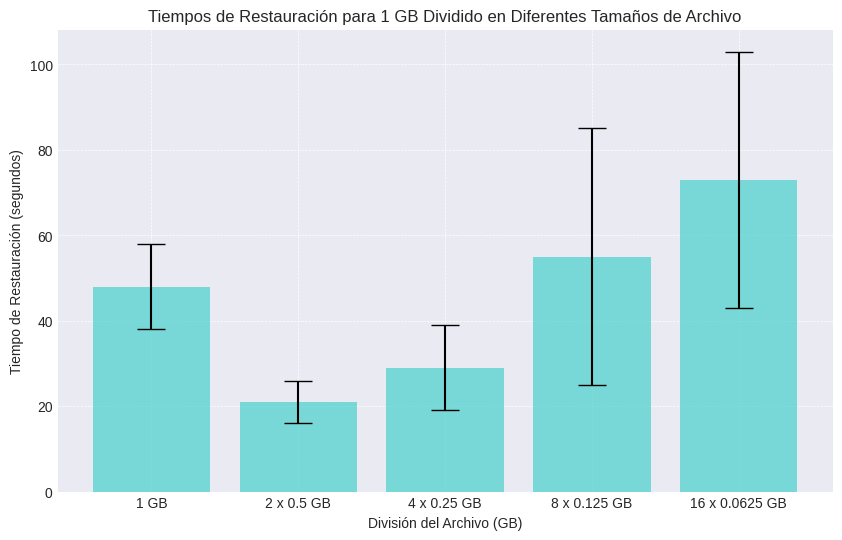
\includegraphics[width=0.8\textwidth]{tiempo_de_restauracion.png}
    \caption{Tiempos de Restauración para 1 GB Dividido en Diferentes Tamaños de Archivo}
    \label{fig:tiempo-restauracion-fraccion}
\end{figure}

\textbf{Descripción de los Datos:}
Los datos muestran que al dividir un archivo de 1 GB en fracciones más pequeñas, el tiempo de restauración varía. Para un solo archivo de 1 GB, el tiempo de restauración es de aproximadamente 48 segundos con una desviación estándar considerable. Cuando se divide en dos archivos de 0.5 GB, el tiempo de restauración disminuye a aproximadamente 21 segundos. Al dividirse en cuatro archivos de 0.25 GB, el tiempo de restauración sube ligeramente a unos 29 segundos. La división en ocho archivos de 0.125 GB resulta en un tiempo de restauración de aproximadamente 55 segundos con una desviación estándar considerable. Finalmente, la división en dieciséis archivos de 0.0625 GB muestra un tiempo de restauración de unos 73 segundos con una desviación estándar también significativa.

\textbf{Análisis de Resultados:}
Los resultados indican que el tiempo de restauración no varía linealmente con la división del archivo de 1 GB en fracciones más pequeñas. La restauración de un archivo grande único o de pocas fracciones grandes tiende a ser más rápida en comparación con la restauración de múltiples fracciones pequeñas. Esto se debe a que la restauración de archivos pequeños implica más operaciones de entrada y salida, así como mayor sobrecarga administrativa, lo que incrementa el tiempo total de restauración.



 %%%%%%%%%%%%%%%


  \subsection{Resultados del Uso de Recursos durante el Backup}

En este apartado se presentan los resultados obtenidos al medir el uso de recursos (CPU y memoria) durante la ejecución de un job de backup, comparado con el uso de recursos en estado baseline. La Figura \ref{fig:uso-recursos} muestra el uso de CPU y memoria en el cliente y el servidor antes y durante la ejecución del job de backup.

\begin{figure}[H]
    \centering
    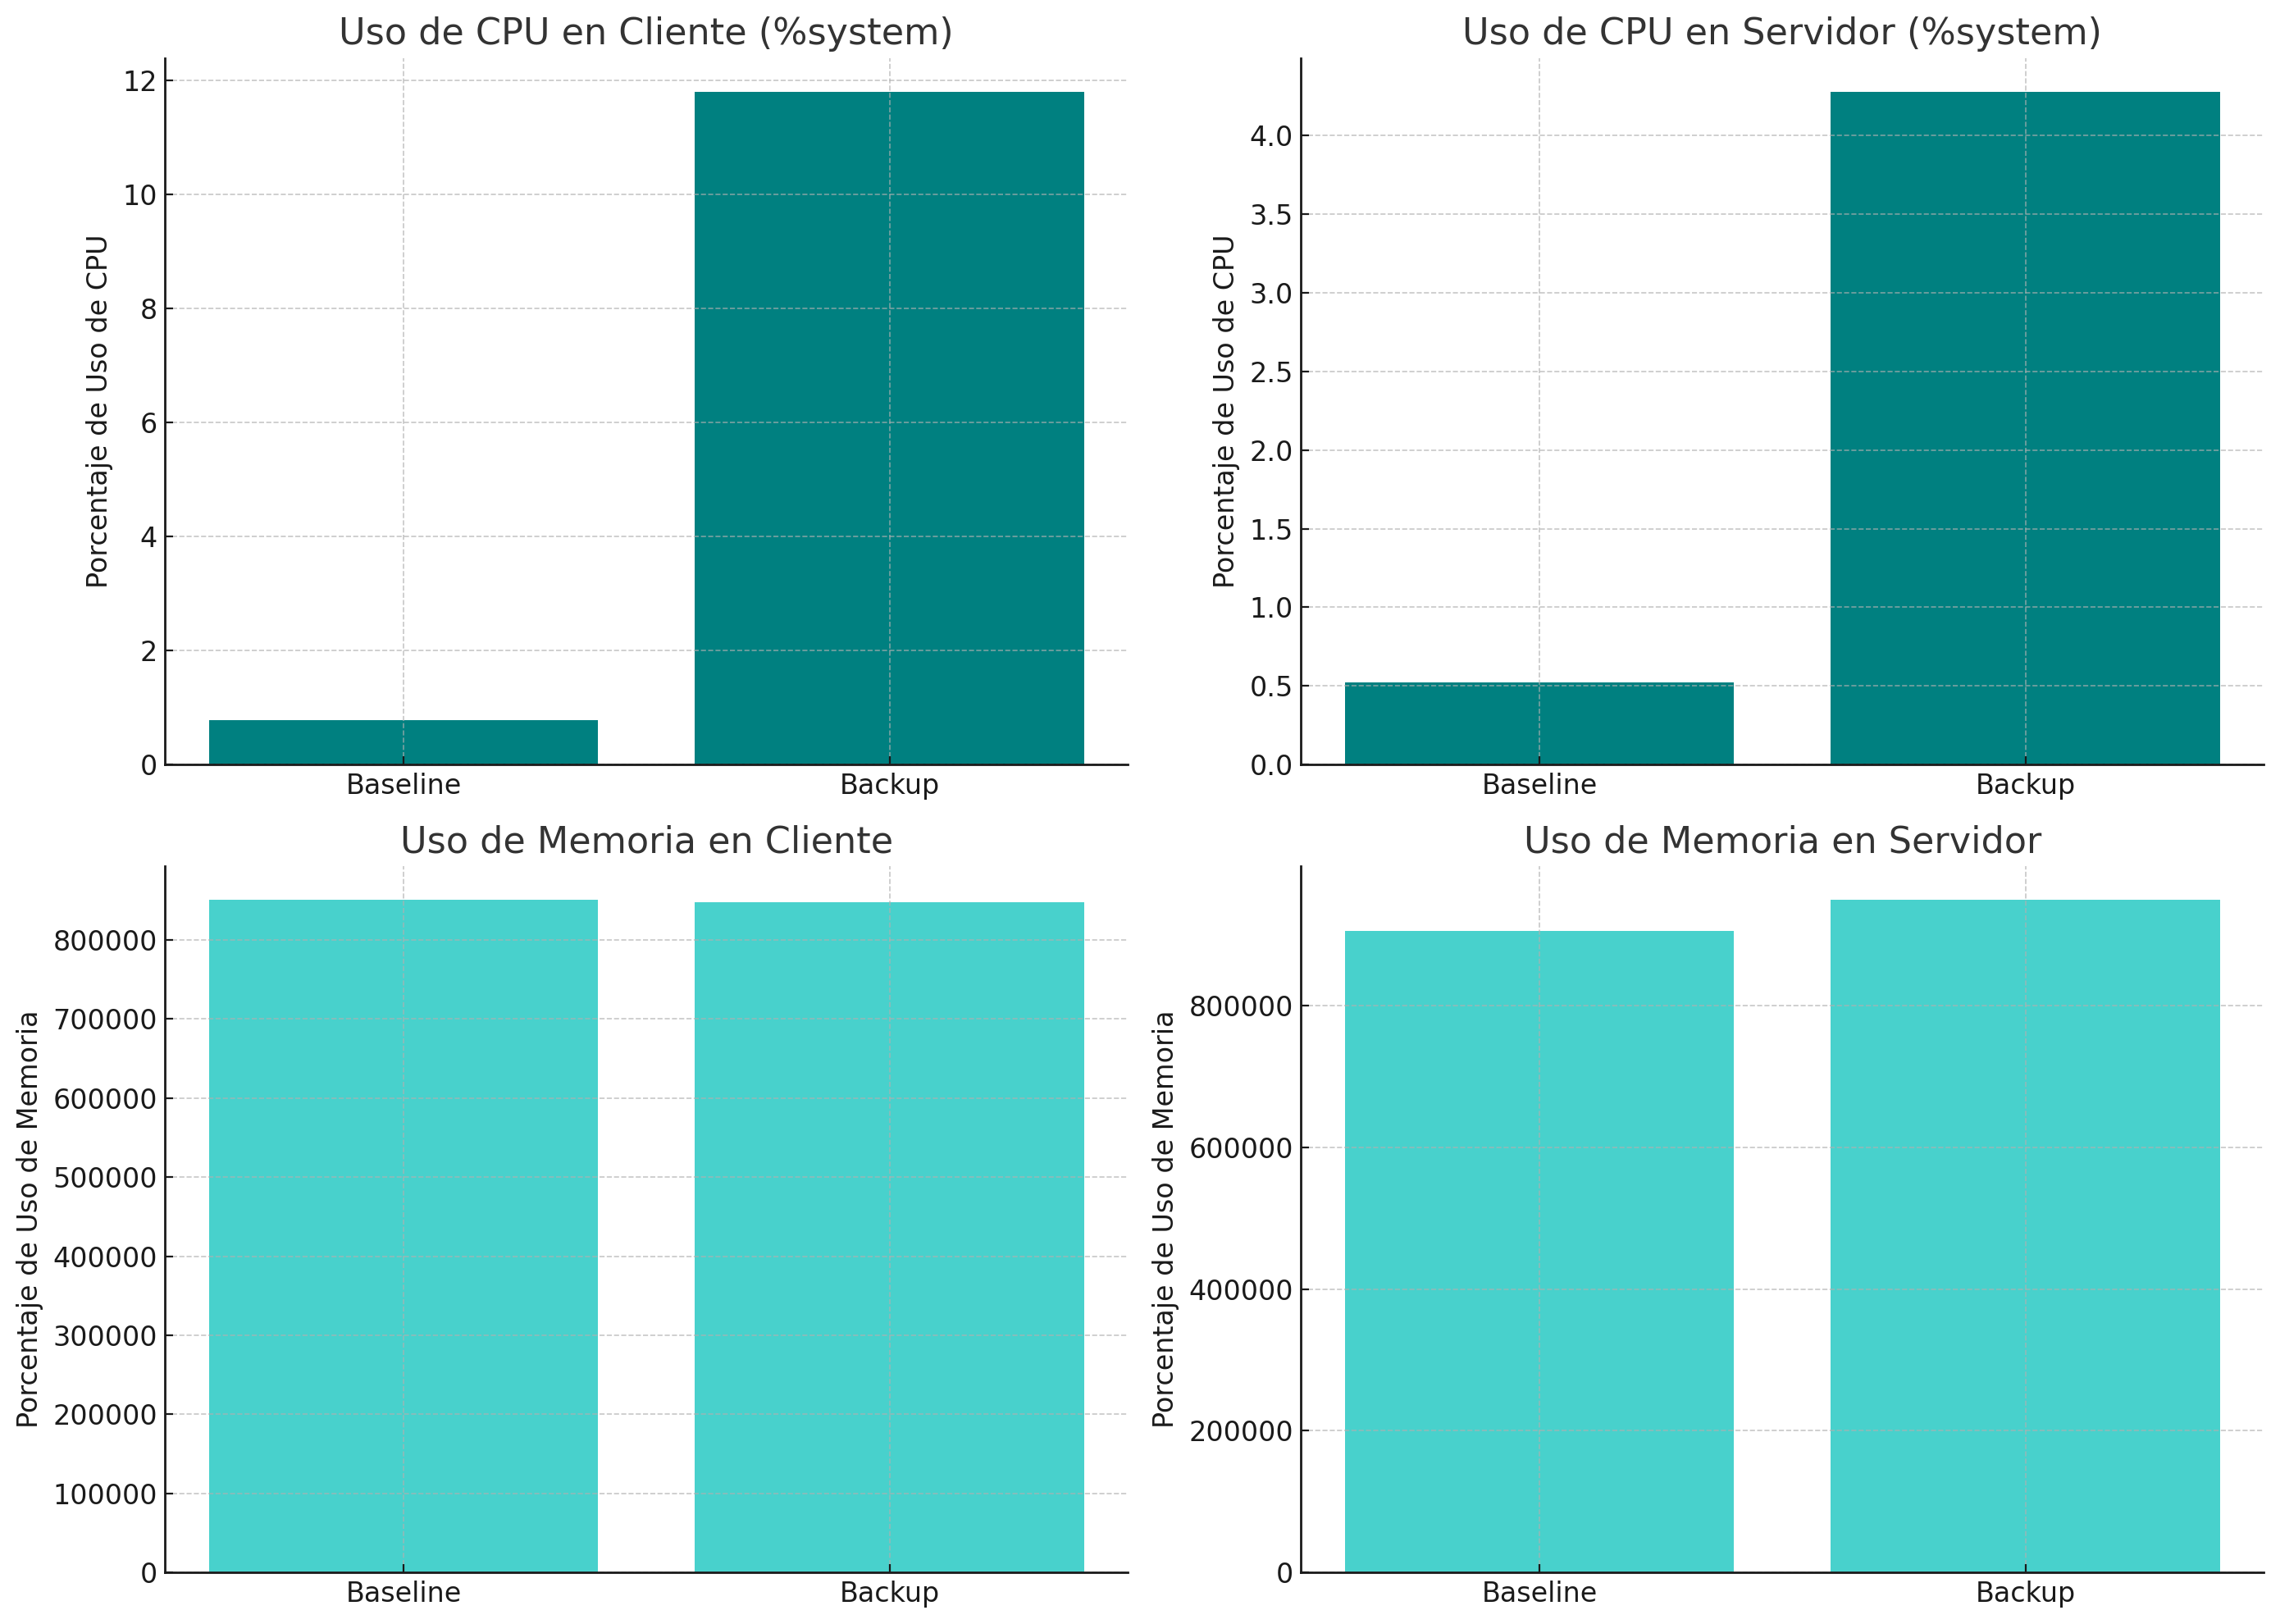
\includegraphics[width=0.8\textwidth]{uso_de_recursos.png}
    \caption{Uso de Recursos durante el Backup}
    \label{fig:uso-recursos}
\end{figure}

\textbf{Descripción de los Datos:}
Los gráficos muestran el uso de CPU (\%system) y memoria en el cliente y en el servidor en dos condiciones: estado baseline y durante el backup.

\textbf{Uso de CPU en el Cliente:}
- En estado baseline, el uso de CPU (\%system) es bajo, alrededor del 1\%.
- Durante el backup, el uso de CPU (\%system) aumenta al 12\%.

\textbf{Uso de CPU en el Servidor:}
- En estado baseline, el uso de CPU (\%system) es alrededor del 0.5\%.
- Durante el backup, el uso de CPU (\%system) se incrementa al 4\%.

\textbf{Uso de Memoria en el Cliente:}
- En estado baseline, el uso de memoria es aproximadamente 820,000 KB.
- Durante el backup, el uso de memoria se mantiene casi constante en aproximadamente 820,000 KB.

\textbf{Uso de Memoria en el Servidor:}
- En estado baseline, el uso de memoria es alrededor de 820,000 KB.
- Durante el backup, el uso de memoria también se mantiene constante en alrededor de 820,000 KB.

\textbf{Análisis de Resultados:}
Los resultados indican que, aunque hay un incremento notable en el uso de CPU (\%system) tanto en el cliente como en el servidor durante el backup, el uso de memoria se mantiene prácticamente constante. Esto sugiere que Bacula, aunque intensivo en el uso de CPU durante los procesos de backup, es eficiente en términos de uso de memoria.
\smallskip
A pesar del incremento en el uso de CPU durante el backup, Bacula utiliza relativamente pocos recursos en comparación con su funcionalidad. El aumento en el uso de CPU es esperado debido a la naturaleza del procesamiento de datos y la escritura en almacenamiento, pero es manejable dentro de los recursos disponibles del sistema. El uso constante de memoria sugiere que Bacula gestiona eficientemente la carga de trabajo sin causar picos significativos en el consumo de memoria, lo que es beneficioso para la estabilidad del sistema y la ejecución de otras tareas concurrentes.


%%%%%%%%%%%%5%%

\subsection{Resultados del Efecto del Número de Jobs en el Tiempo de Backup de 1 GB}

En este apartado se presentan los resultados obtenidos al medir el tiempo de backup de 1 GB en función del número de jobs. La Figura \ref{fig:efecto-numero-jobs} muestra cómo varía el tiempo de backup a medida que se incrementa el número de jobs simultáneos.

\begin{figure}[H]
    \centering
    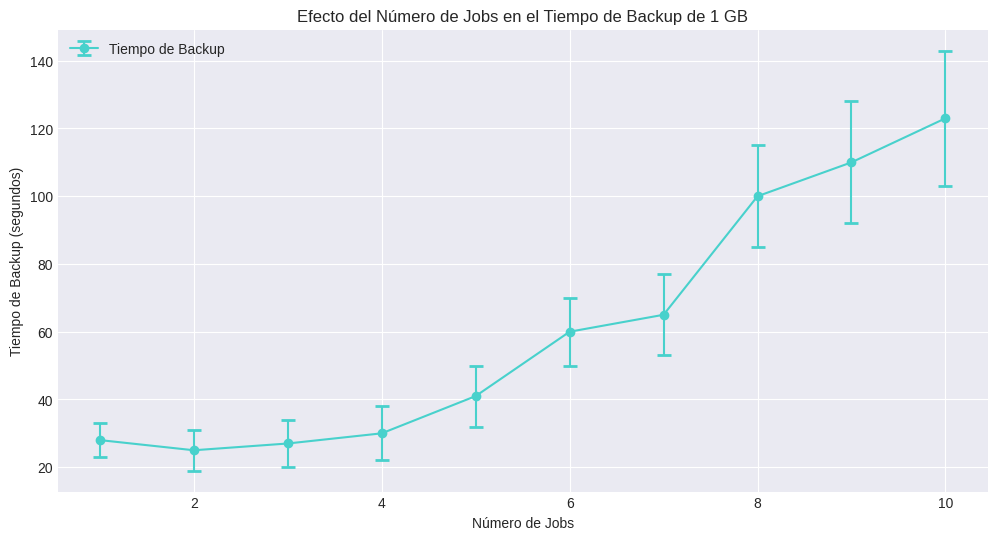
\includegraphics[width=0.8\textwidth]{efecto_numero_jobs.png}
    \caption{Efecto del Número de Jobs en el Tiempo de Backup de 1 GB}
    \label{fig:efecto-numero-jobs}
\end{figure}

\textbf{Descripción de los Datos:}
Los datos muestran que a medida que aumenta el número de jobs simultáneos, el tiempo de backup también incrementa. Con un solo job, el tiempo de backup es de aproximadamente 28 segundos. Cuando se incrementa a dos jobs, el tiempo se mantiene casi constante, pero a partir de cuatro jobs se observa un incremento progresivo en el tiempo de backup, alcanzando aproximadamente 142 segundos con diez jobs.

\textbf{Análisis de Resultados:}
Los resultados indican que hay un punto de inflexión en el cual el incremento del número de jobs comienza a afectar significativamente el tiempo de backup. Hasta cuatro jobs, el tiempo de backup incrementa de manera moderada, pero a partir de seis jobs, el incremento es más pronunciado. Esto sugiere que hay una sobrecarga en el sistema cuando se maneja un alto número de jobs simultáneamente, probablemente debido a la competencia por los recursos del sistema, como la CPU y el I/O de disco.

\textbf{Comportamiento Observado:}
El incremento en el tiempo de backup con el número de jobs puede explicarse por la limitación de los recursos del sistema. Cada job adicional compite por los mismos recursos, lo que puede causar congestión y aumentar el tiempo necesario para completar cada backup. Este comportamiento es consistente con lo esperado en sistemas donde los recursos son compartidos y limitados.






\subsection{Resultados de la Estabilidad Temporal de Tiempos de Backup de 1 GB cada 2 Minutos}

En este apartado se presentan los resultados obtenidos al medir la estabilidad temporal de los tiempos de backup para un archivo de 1 GB realizado cada 2 minutos durante un período de 9 horas y 16 minutos. La Figura \ref{fig:estabilidad-temporal} muestra los tiempos de backup en función del tiempo transcurrido.

\begin{figure}[H]
    \centering
    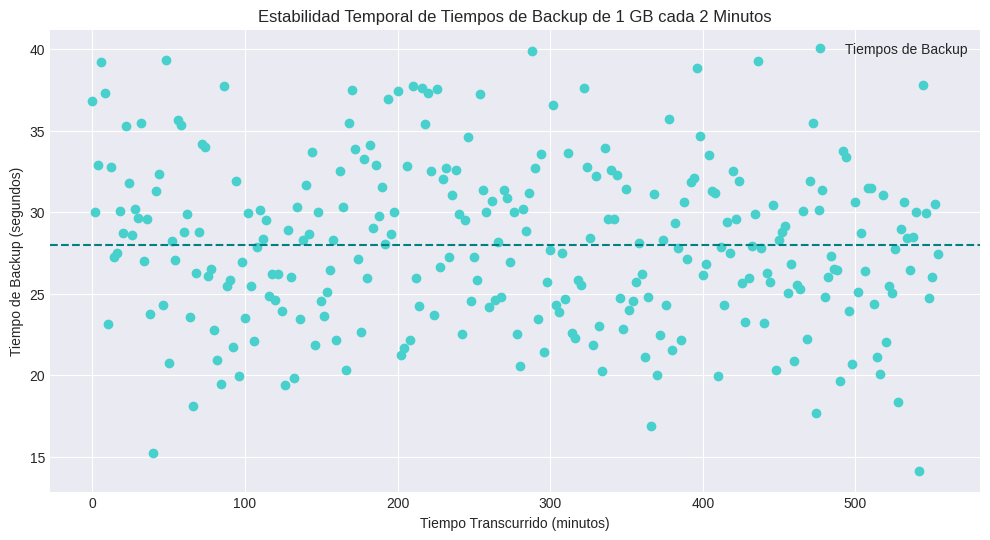
\includegraphics[width=0.8\textwidth]{estabilidad_temporal.png}
    \caption{Estabilidad Temporal de Tiempos de Backup de 1 GB cada 2 Minutos}
    \label{fig:estabilidad-temporal}
\end{figure}

\textbf{Descripción de los Datos:}
Los datos muestran los tiempos de backup de 1 GB medidos cada 2 minutos durante el período de estudio. La gráfica presenta una dispersión de los tiempos de backup alrededor de un valor medio de aproximadamente 28 segundos, con variaciones entre 15 y 40 segundos.

\textbf{Análisis de Resultados:}
Los resultados indican que los tiempos de backup tienen una variabilidad moderada alrededor del valor medio. A lo largo del período de 9 horas y 16 minutos, no se observa una tendencia clara de incremento o decremento en los tiempos de backup, lo que sugiere una estabilidad temporal razonable. La línea punteada en la gráfica representa el valor medio de los tiempos de backup, proporcionando una referencia visual para evaluar la dispersión de los datos.

\textbf{Comportamiento Observado:}
La dispersión de los tiempos de backup puede atribuirse a variaciones en la carga del sistema y en el rendimiento de los recursos compartidos durante el período de estudio. Factores como la actividad de otros procesos, la fluctuación en el rendimiento del almacenamiento y las condiciones de red pueden influir en los tiempos de backup observados. Sin embargo, la falta de una tendencia clara sugiere que el sistema de backup mantiene una consistencia razonable en sus tiempos de operación bajo las condiciones de prueba.


\subsection{Costes de implementación de la Estrategia 3-2-1 en Bacula}

En este apartado se describe la implementación de la estrategia 3-2-1 junto con la estrategia GFS en Bacula, aplicada en la empresa donde trabajo. En esta empresa, utilizamos alrededor de 2 GB mensuales de backup. La implementación se realizará usando un servidor local, una unidad de cinta y almacenamiento en la nube.

\textbf{Tres copias de datos:}
\begin{itemize}
    \item \textbf{Copia 1:} Servidor local.
    \item \textbf{Copia 2:} Cinta.
    \item \textbf{Copia 3:} Nube.
\end{itemize}




\textbf{Cálculo del Almacenamiento Necesario}
\begin{itemize}
    \item \textbf{Cantidad de datos generados:}
    \begin{itemize}
        \item Datos mensuales: 2GB.
        \item Datos anuales: 2GB * 12 meses = 24GB.
        \item Datos en 5 años: 24GB * 5 años = 120GB.
        \item Con un 20\% de margen = 150GB.
    \end{itemize}

    \item \textbf{Estrategia GFS:}
    \begin{itemize}
        \item Backups diarios (incrementales): se retienen aproximadamente 1 semana.
        \item Backups semanales (diferenciales): se retienen aproximadamente 1 mes.
        \item Backups mensuales (completos): se retienen aproximadamente 5 años.
    \end{itemize}
\end{itemize}

Para los cálculos, asumimos que los incrementales y diferenciales son una fracción del tamaño de los completos.

\textbf{Implementación}
\begin{enumerate}
    \item \textbf{Servidor Local}
    \begin{itemize}
        \item \textbf{Hardware:} Servidor con almacenamiento (Fujitsu Primergy Server TX1310 M5 Intel Xeon E-2324G/8GB/2TB).
        \item \textbf{RAID:} 2TB (considerando crecimiento futuro y espacio para snapshots, logs, etc.).
        \item \textbf{Memoria RAM:} 8GB.
    \end{itemize}
    \textbf{Costos aproximados:}
    \begin{itemize}
        \item Servidor: €986,58 \footnote{https://www.pccomponentes.com/fujitsu-primergy-server-tx1310-m5-intel-xeon-e-2324g-8gb-2tb}.
        \item Coste de electricidad: 209 W con un consumo eléctrico de 5.016 kWh y un coste total de €0.25 diarios.
    \end{itemize}

    \item \textbf{Unidad de Cinta}
    \begin{itemize}
        \item \textbf{Hardware:} Unidad de cinta LTO.
    \end{itemize}
    \textbf{Costos aproximados:}
    \begin{itemize}
        \item Unidad LTO: en torno a los €2000.
        \item Cintas LTO (12TB): €50 cada una.
    \end{itemize}

    \item \textbf{Almacenamiento en la Nube}
    \begin{itemize}
        \item \textbf{Proveedor de nube:} AWS S3, Google Cloud Storage, Azure Blob Storage.
    \end{itemize}
    \textbf{Costos aproximados:}
    \begin{itemize}
        \item Costo por almacenamiento en la nube (150GB): Aproximadamente €0.023/GB al mes.
    \end{itemize}
\end{enumerate}

\textbf{Resumen de Costos:}
\begin{itemize}
    \item \textbf{Servidor Local:}
    \begin{itemize}
        \item Costo inicial del servidor: €986,58.
        \item Costo anual de electricidad: €0.25 * 365 = €91.25.
    \end{itemize}
    \item \textbf{Unidad de Cinta:}
    \begin{itemize}
        \item Costo inicial de la unidad LTO: aproximadamente €2000.
        \item Costo de cintas LTO: Asumiendo un total de 150GB, necesitaríamos 1 cintas , lo que sería  €50.
    \end{itemize}
    \item \textbf{Almacenamiento en la Nube:}
    \begin{itemize}
        \item Costo mensual: 150GB * €0.023 = €3.45.
        \item Costo anual: €3.45 * 12 = €41.4.
    \end{itemize}
\end{itemize}

La implementación de la estrategia 3-2-1 junto con la estrategia GFS en Bacula, aunque implica un costo inicial considerable para el hardware y el almacenamiento, asegura la redundancia y la seguridad de los datos. Esta estrategia garantiza que los datos estén protegidos contra fallos del sistema, desastres y otros eventos imprevistos, ofreciendo una solución robusta y fiable para la gestión de backups en la empresa.











\section{Conclusiones y trabajos futuros}


\subsection{Conclusiones}

En este apartado se presentan las conclusiones del trabajo realizado, centrado en analizar las capacidades y configuraciones óptimas de Bacula para la protección contra ransomware. Los objetivos específicos del trabajo eran: analizar las capacidades y configuraciones óptimas de Bacula para la protección contra ransomware, implementar un entorno de prueba con Bacula, desarrollar una guía de mejores prácticas para el uso de Bacula en la protección contra ransomware y evaluar la viabilidad y eficiencia de la solución propuesta.

\textbf{Análisis de las Capacidades y Configuraciones Óptimas de Bacula:}
\begin{itemize}
    \item Bacula ofrece una amplia gama de capacidades para la protección contra ransomware, incluyendo la capacidad de realizar backups incrementales, diferenciales y completos, así como la opción de implementar estrategias de backup avanzadas como la estrategia GFS o la estrategia 3-2-1.
    \item La flexibilidad de configuración de Bacula permite ajustar los parámetros de compresión, retención y replicación de datos para maximizar la eficiencia del backup y la protección de los datos.
    \item La implementación de la estrategia 3-2-1, junto con la estrategia GFS, asegura una alta redundancia y seguridad de los datos, proporcionando múltiples copias en diferentes tipos de medios y ubicaciones.
\end{itemize}

\textbf{Implementación de un Entorno de Prueba con Bacula:}
\begin{itemize}
    \item Se implementó un entorno de prueba con Bacula que incluyó la configuración de varios servidores locales, para probar su robustez frente a sistemas operativos Linux, windows y copias de bases de datos.
    \item Los resultados de las pruebas mostraron que Bacula es capaz de manejar eficientemente los procesos de backup y restauración, manteniendo una estabilidad temporal adecuada y un uso razonable de los recursos del sistema.
    \item Las pruebas de velocidad de backup y restauración para diferentes tamaños de archivos y configuraciones de compresión demostraron la capacidad de Bacula para adaptarse a diversas necesidades y escenarios.
\end{itemize}

\textbf{Guía de Mejores Prácticas para el Uso de Bacula:}
\begin{itemize}
    \item Se desarrolló una guía de mejores prácticas que incluye recomendaciones para la configuración óptima de Bacula, la implementación de estrategias de backup y la gestión de la seguridad de los datos.
    \item La guía destaca la importancia de la implementación de la estrategia 3-2-1 y la estrategia GFS para asegurar la redundancia y protección de los datos.
    \item También se incluyen recomendaciones para la optimización del uso de recursos y la minimización del impacto en el rendimiento del sistema durante los procesos de backup y restauración.
\end{itemize}

\textbf{Evaluación de la Viabilidad y Eficiencia de la Solución Propuesta:}
\begin{itemize}
    \item La solución propuesta demostró ser viable y eficiente para la protección contra ransomware en un entorno empresarial.
    \item Los costos asociados a la implementación de la estrategia 3-2-1 y la estrategia GFS, aunque significativos, son justificables por la alta redundancia y seguridad que ofrecen.
    \item La implementación de Bacula, junto con las estrategias de backup recomendadas, proporciona una solución robusta y confiable para la protección de datos críticos contra amenazas de ransomware y otros desastres.
\end{itemize}

\textbf{Conclusiones Generales:}

Los datos resaltan la importancia de considerar el tamaño de los archivos y el tamaño del pool de almacenamiento al planificar estrategias de backup. Para archivos pequeños, el impacto en el tiempo de backup es mínimo, pero para archivos grandes, una infraestructura bien dimensionada es esencial para mantener los tiempos de backup dentro de rangos aceptables. Además, es importante tener en cuenta la creciente incertidumbre en la medida del tiempo de backup para archivos más grandes, lo que puede afectar la previsibilidad y la planificación del proceso de backup.

Estos resultados sirven como guía para optimizar la configuración del sistema de backup, asegurando que los recursos disponibles sean utilizados de manera eficiente y efectiva. Los resultados sugieren que la división de archivos grandes en fracciones más pequeñas puede incrementar el tiempo total de backup debido a la sobrecarga adicional en la gestión de archivos. Además, la variabilidad en los tiempos de backup se incrementa con el número de fracciones, lo que puede afectar la predictibilidad del tiempo de backup. Estos hallazgos destacan la importancia de optimizar la estrategia de división de archivos y considerar los recursos del sistema disponibles para minimizar el impacto en el tiempo de backup.

Al planificar estrategias de backup, es crucial considerar el trade-off entre el nivel de compresión y el tiempo de respaldo. GZIP, aunque más lento, puede reducir significativamente el espacio de almacenamiento necesario, lo que es beneficioso para archivos grandes. Por otro lado, LZO proporciona tiempos de respaldo más rápidos, lo que puede ser ventajoso en entornos donde la velocidad es prioritaria. Estos hallazgos ayudan a guiar la elección de algoritmos de compresión según las necesidades específicas de almacenamiento y tiempo de respaldo.

Los datos resaltan la importancia de considerar los tiempos de restauración al planificar estrategias de backup y recuperación. Aunque el tiempo de backup es crucial, el tiempo de restauración es igualmente importante, especialmente en escenarios donde la restauración rápida de datos es crítica. Estos resultados subrayan la necesidad de optimizar tanto el proceso de backup como el de restauración para asegurar que se puedan cumplir los requisitos de recuperación en un tiempo razonable.

Estos resultados resaltan la eficiencia de Bacula en términos de uso de recursos. Aunque el backup es una operación intensiva en CPU, Bacula maneja esta carga de manera efectiva sin impactar significativamente el uso de memoria. Esto es crucial para mantener el rendimiento general del sistema mientras se realizan operaciones de backup, permitiendo que otros procesos continúen funcionando sin interrupciones notables.

Finalmente, los datos resaltan la importancia de optimizar el número de jobs simultáneos para maximizar la eficiencia del backup. Mientras que un pequeño número de jobs no impacta significativamente el tiempo de backup, un número mayor de jobs puede causar un incremento exponencial en el tiempo necesario para completar el backup. Esto sugiere que es crucial encontrar un equilibrio entre la cantidad de trabajos paralelos y la capacidad del sistema para manejarlos eficientemente.

En resumen, el trabajo realizado demuestra que Bacula es una herramienta poderosa y flexible para la gestión de backups y la protección contra ransomware. La implementación de estrategias avanzadas de backup, como la estrategia 3-2-1 y la estrategia GFS, asegura una alta redundancia y seguridad de los datos. La guía de mejores prácticas desarrollada proporciona una base sólida para la configuración y uso óptimo de Bacula en entornos empresariales, asegurando la viabilidad y eficiencia de la solución propuesta para la protección contra ransomware.




\subsection{Trabajos Futuros}

A partir de los resultados obtenidos y las conclusiones alcanzadas en este trabajo, se identifican diversas áreas para futuras investigaciones y mejoras en la implementación de Bacula como herramienta de backup y protección contra ransomware. Los trabajos futuros se pueden agrupar en las siguientes áreas:

\textbf{1. Despliegue Automático:}
\begin{itemize}
    \item \textbf{Automatización del Despliegue:} Desarrollar y probar scripts y herramientas para la automatización del despliegue de Bacula en diferentes entornos. Esto incluye la creación de configuraciones automatizadas para la instalación, configuración y actualización de los componentes de Bacula.
    \item \textbf{Integración con Herramientas de Gestión:} Integrar Bacula con herramientas de gestión de configuración como Ansible, Puppet o Chef para facilitar la implementación y el mantenimiento de la infraestructura de backup.
\end{itemize}

\textbf{2. Implementación de Backup/Restore con Cintas LTO:}
\begin{itemize}
    \item \textbf{Pruebas de Rendimiento y Confiabilidad:} Implementar y evaluar el uso de cintas LTO para los procesos de backup y restore en la empresa. Realizar pruebas de rendimiento y confiabilidad para asegurar que las cintas LTO proporcionen una solución robusta y eficiente.
    \item \textbf{Optimización de la Estrategia de Backup:} Ajustar las estrategias de backup para maximizar la eficiencia del uso de cintas LTO, incluyendo la programación de backups completos, incrementales y diferenciales.
\end{itemize}

\textbf{3. Complementar el Sistema de Backup con Otras Medidas de Defensa:}
\begin{itemize}
    \item \textbf{Integración con Soluciones de Seguridad:} Complementar el sistema de backup con soluciones avanzadas de seguridad, como sistemas de detección y respuesta ante amenazas (EDR), protección contra malware y firewalls de próxima generación.
    \item \textbf{Evaluación de Medidas Adicionales:} Evaluar e implementar medidas adicionales de defensa, como la segmentación de red, la autenticación multifactor y la formación de los empleados en prácticas de seguridad cibernética, para crear un sistema completo de protección de datos.
\end{itemize}

\newpage
\pagenumbering{Roman} 
\section{Glosario}
\textbf{Bacula:} Bacula es un conjunto de programas de respaldo (backup) de código abierto que permite gestionar backups, restauraciones y verificaciones de datos a través de una red de computadoras.

\textbf{Ransomware:} El ransomware es un tipo de software malicioso que cifra los archivos de la víctima, exigiendo un rescate para restaurar el acceso a los datos.

\textbf{Backup:} Copia de seguridad de datos que se utiliza para restaurar los datos originales en caso de pérdida de datos.

\textbf{Restore:} Proceso de recuperación de datos a partir de un backup.

\textbf{GFS:} Grandfather-Father-Son, una estrategia de rotación de copias de seguridad que implica realizar backups diarios (Son), semanales (Father) y mensuales (Grandfather).

\textbf{3-2-1:} Estrategia de backup que recomienda tener tres copias de los datos en dos tipos de medios diferentes, con al menos una copia fuera del sitio.

\textbf{Backup Incremental:} Tipo de backup que copia solo los datos que han cambiado desde el último backup.

\textbf{Backup Diferencial:} Tipo de backup que copia todos los datos que han cambiado desde el último backup completo.

\textbf{Backup Completo:} Tipo de backup que copia todos los datos seleccionados independientemente de cuándo se modificaron por última vez.

\textbf{Compresión:} Proceso de reducir el tamaño de los datos para ahorrar espacio de almacenamiento o ancho de banda.

\textbf{LTO:} Linear Tape-Open, una tecnología de cinta magnética utilizada para almacenamiento de datos a largo plazo.

\textbf{AWS S3:} Amazon Web Services Simple Storage Service, un servicio de almacenamiento en la nube que ofrece escalabilidad, alta disponibilidad y seguridad de datos.

\textbf{Demonio:} Un programa que se ejecuta en segundo plano y realiza tareas específicas, como el backup o la restauración de datos en Bacula.

\textbf{Cliente:} En Bacula, un cliente es un sistema que se respalda y que tiene el Bacula File Daemon (FD) instalado para comunicar con el Director.

\textbf{Trabajo:} Una tarea o job en Bacula, que especifica una operación de backup, restauración o verificación de datos.

\textbf{MD5:} Algoritmo de hash que produce un valor de resumen de 128 bits a partir de un archivo o mensaje, utilizado para asegurar la integridad de los datos.

\textbf{Autentificación TLS:} Transport Layer Security, un protocolo que proporciona comunicaciones seguras a través de una red mediante la autenticación y el cifrado.

\textbf{Pool:} Un grupo de volúmenes de almacenamiento que Bacula utiliza para organizar y gestionar los backups.

\textbf{FileExistsError:} Un error que se produce cuando se intenta crear un archivo que ya existe en el sistema.

\textbf{Schedule:} Programación de tareas en Bacula, que define cuándo deben ejecutarse los trabajos de backup.

\textbf{Pipe:} Un método para redirigir la salida de un comando como entrada a otro comando, útil en procesos de backup y restauración.

\textbf{Catálogo de Bacula:} Base de datos que almacena la información sobre los archivos respaldados, los volúmenes de almacenamiento y el estado de los trabajos en Bacula.

\textbf{Concurrencia y Multitasking:} La capacidad de Bacula para ejecutar múltiples tareas o trabajos de backup simultáneamente.

\textbf{Logs:} Registros detallados de eventos y actividades del sistema, utilizados para monitorear y solucionar problemas en Bacula.

\textbf{SLAs:} Service Level Agreements, acuerdos de nivel de servicio que definen los niveles de servicio esperados, incluyendo tiempos de backup y restauración.

\textbf{SSDs:} Solid State Drives, dispositivos de almacenamiento de datos que utilizan memoria flash para proporcionar tiempos de acceso rápidos.

\textbf{Deduplicación:} Tecnología que reduce el almacenamiento necesario eliminando copias redundantes de datos.

\textbf{CPU:} Unidad Central de Procesamiento, el componente principal de un ordenador que realiza las operaciones de procesamiento de datos.

\textbf{Memoria:} Dispositivo de almacenamiento temporal en un ordenador, utilizado para guardar datos y programas en uso.

\newpage
%========================================================================%$$
%                                                                        %$$
%                          Bibliografia                                  %$$
%                                                                        %$$
%========================================================================%$$
                                                                         %$$
\section{Bibliografía}                                                   %$$
\printbibliography                                                       %$$
                                                                         %$$
%************************************************************************%$$
%                                                                        %$$
%                          Fin Bibliografia                              %$$
%                                                                        %$$
%========================================================================%$$





\newpage

%========================================================================%$$
%                                                                        %$$
%                                Anexos                                  %$$
%                                                                        %$$
%========================================================================%$$
                                                                         %$$
\section{Anexos}                                                         %$$ 





\subsection{Instalación de Debian}                                       %$$

\textbf{Descarga de la Imagen de Instalación}
\medskip

Primero, descargamos la imagen de Debian adecuada para nuestras necesidades. Para ello, visitamos la página oficial de Debian en \url{https://www.debian.org/distrib/} y seleccionamos la imagen de instalación que mejor se adapte a nuestro caso. En este ejemplo, se eligió la imagen de instalación a través de Internet.

\begin{figure}[H]
    \centering
    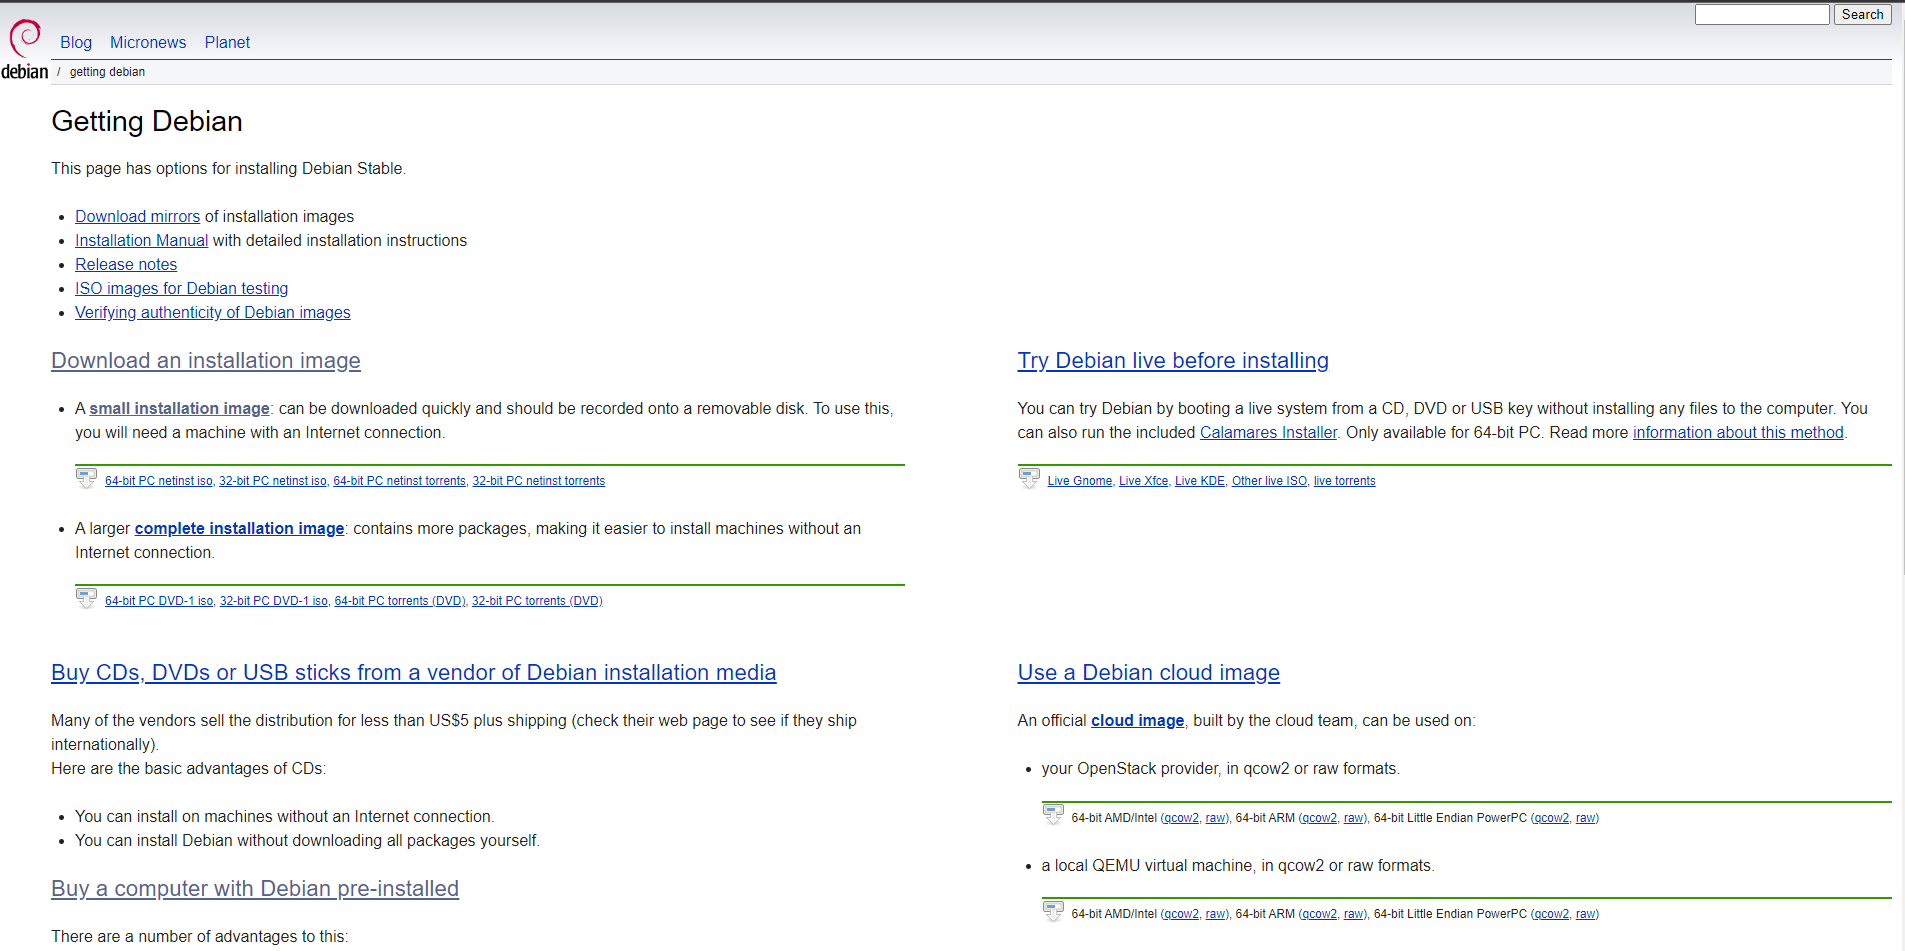
\includegraphics[width=0.5\linewidth]{instalacionBacula/debianPaginaWeb.png}
    \caption{Página de descarga de Debian}
\end{figure}

\textbf{Creación de la Máquina Virtual}\medskip


En VirtualBox, procedemos a añadir una nueva máquina virtual. Asignamos un nombre a la máquina y seleccionamos la imagen ISO de Debian descargada previamente.

\begin{figure}[H]
    \centering
    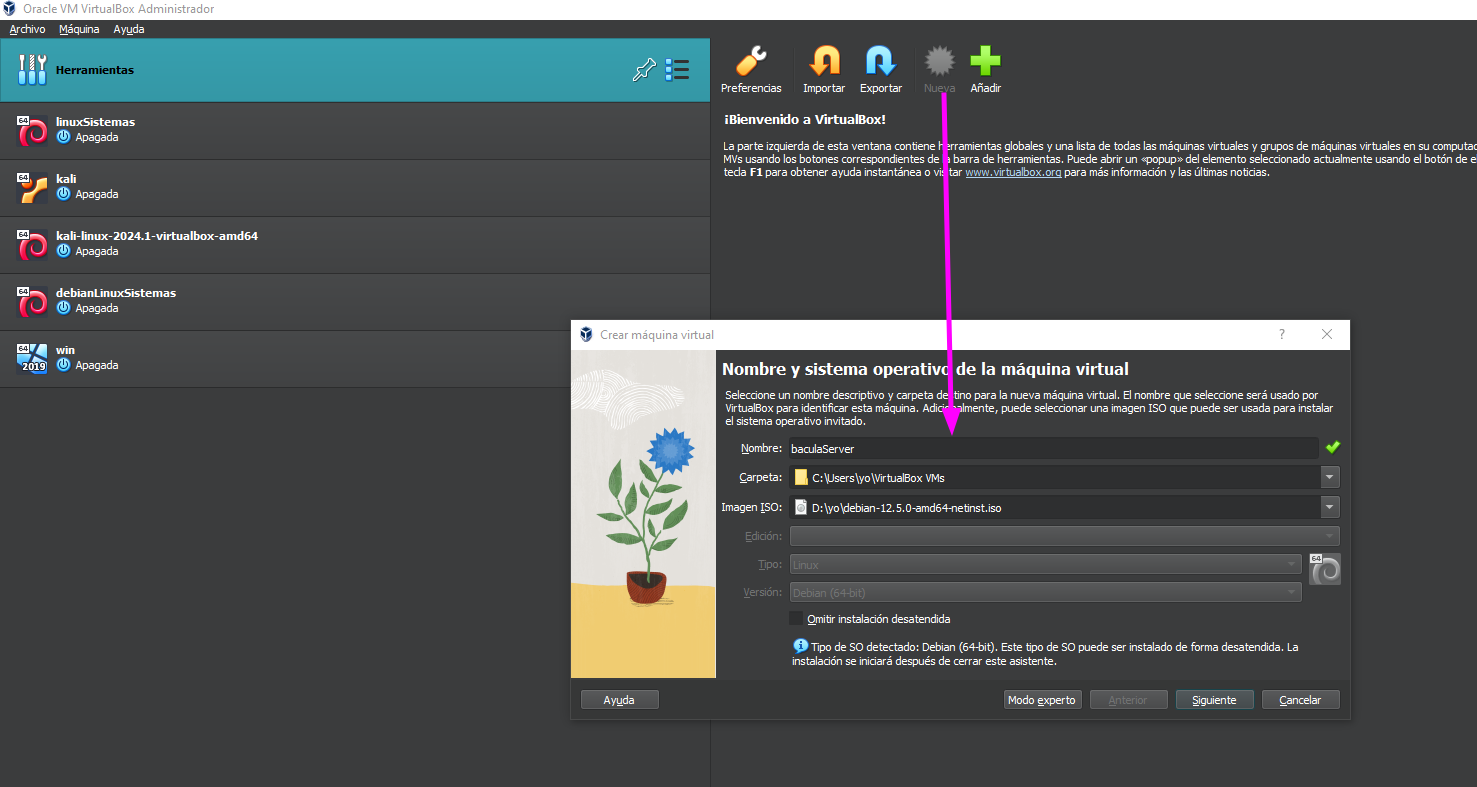
\includegraphics[width=0.5\linewidth]{instalacionBacula/vbDebian.png}
    \caption{Configuración inicial de la máquina virtual en VirtualBox}
\end{figure}

\textbf{Configuración del Usuario y Contraseña}\medskip


Configuramos el usuario y la contraseña que se utilizarán en la máquina virtual.

\begin{figure}[H]
    \centering
    \includegraphics[width=0.5\linewidth]{instalacionBacula/instalación desatendida del SO.png}
    \caption{Establecimiento de usuario y contraseña durante la instalación desatendida}
\end{figure}

\textbf{Configuración del Hardware}\medskip


Debian no requiere muchos recursos para operar de forma fluida. Por tanto, asignamos una cantidad moderada de memoria y procesadores.

\begin{figure}[H]
    \centering
    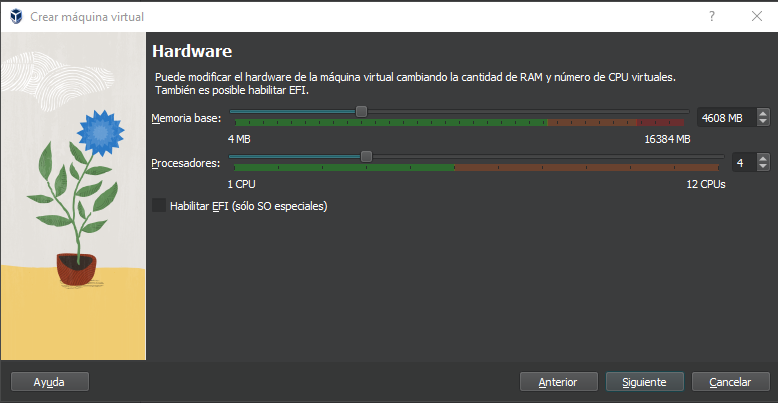
\includegraphics[width=0.5\linewidth]{instalacionBacula/vbhardware.png}
    \caption{Configuración del hardware en VirtualBox}
\end{figure}

\textbf{Asignación de Almacenamiento}\medskip


Creamos un disco duro virtual para la máquina y asignamos un espacio de 50 GB.

\begin{figure}[H]
    \centering
    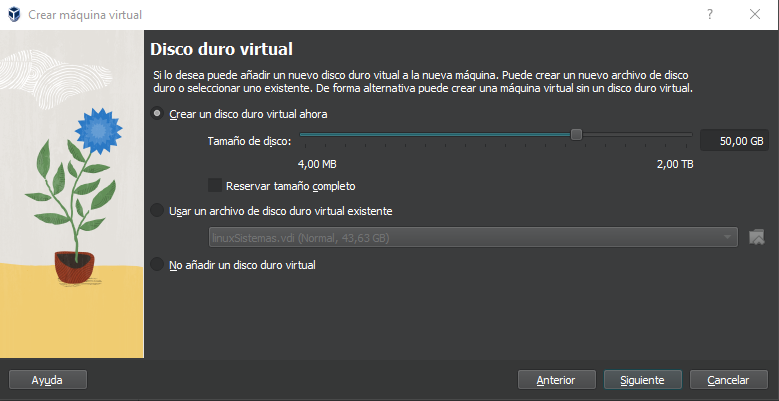
\includegraphics[width=0.5\linewidth]{instalacionBacula/vbDisco.png}
    \caption{Asignación de espacio en el disco duro virtual}
\end{figure}

\textbf{Instalación del Sistema Operativo}\medskip


Iniciamos la instalación de Debian y dejamos que el instalador complete el proceso.

\textbf{Actualización del Sistema}\medskip


Una vez instalado el sistema, ejecutamos comandos de actualización y mejora para asegurarnos de que tenemos la última versión de los paquetes.

\begin{figure}[H]
    \centering
    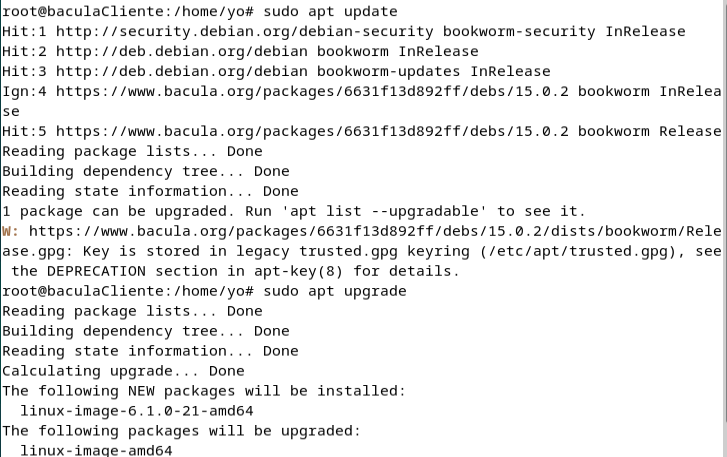
\includegraphics[width=0.5\linewidth]{instalacionBacula/Update y upgrade.png}
    \caption{Proceso de actualización y mejora del sistema}
\end{figure}

\textbf{Configuración de Red}\medskip


Finalmente, ajustamos la configuración de red de NAT a adaptador puente para facilitar la conectividad externa de la máquina virtual.

\begin{figure}[H]
    \centering
    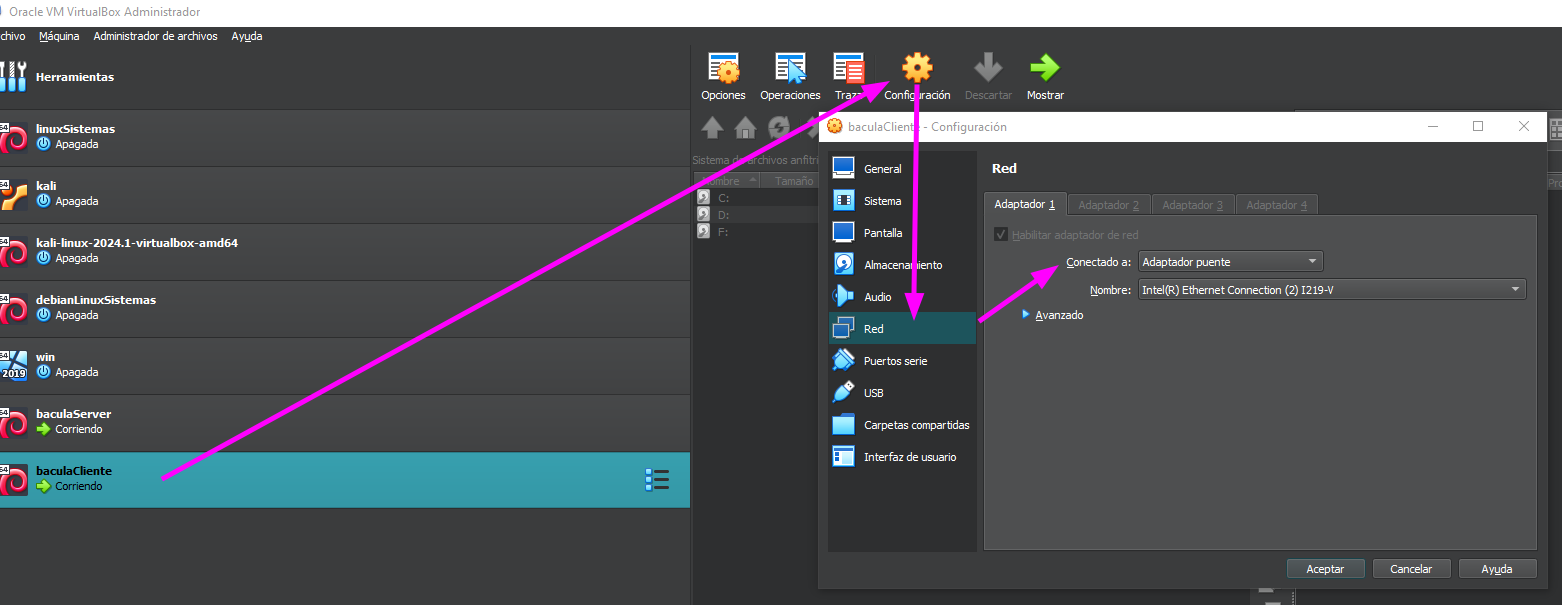
\includegraphics[width=0.5\linewidth]{instalacionBacula/NatAdaptadorPuente.png}
    \caption{Cambio de configuración de red a adaptador puente}
\end{figure}


\subsection{Crear Tabla en la Base de Datos PostgreSQL}

Para comenzar a trabajar con PostgreSQL, primero es necesario instalar el sistema de gestión de base de datos. Para ello, se actualizan los paquetes y se instala PostgreSQL junto con sus contribuciones adicionales utilizando los siguientes comandos:

\begin{verbatim}
sudo apt update
sudo apt upgrade
sudo apt install postgresql postgresql-contrib
\end{verbatim}

Para verificar que el servicio está funcionando correctamente, se pueden utilizar los siguientes comandos:

\begin{verbatim}
sudo systemctl status postgresql
\end{verbatim}

PostgreSQL crea por defecto un usuario llamado \textit{postgres}, que actúa como superusuario del sistema de base de datos. Para comenzar a usar PostgreSQL, primero cambiamos al usuario \textit{postgres} y accedemos a la consola de PostgreSQL con:

\begin{verbatim}
sudo -i -u postgres
psql
\end{verbatim}

Una vez en la consola de PostgreSQL, procedemos a crear una nueva base de datos y una tabla dentro de esta:

\begin{verbatim}
CREATE DATABASE uoc;
\c uoc;
CREATE TABLE uoc (
    id SERIAL PRIMARY KEY,
    nombre VARCHAR(100),
    rol VARCHAR(100)
);
\end{verbatim}

Luego, poblamos la tabla con algunos datos de ejemplo:

\begin{verbatim}
INSERT INTO uoc (nombre, rol) VALUES ('Fernando', 'estudiante');
INSERT INTO uoc (nombre, rol) VALUES ('Rafael', 'profesor');
\end{verbatim}

\begin{figure}[H]
    \centering
    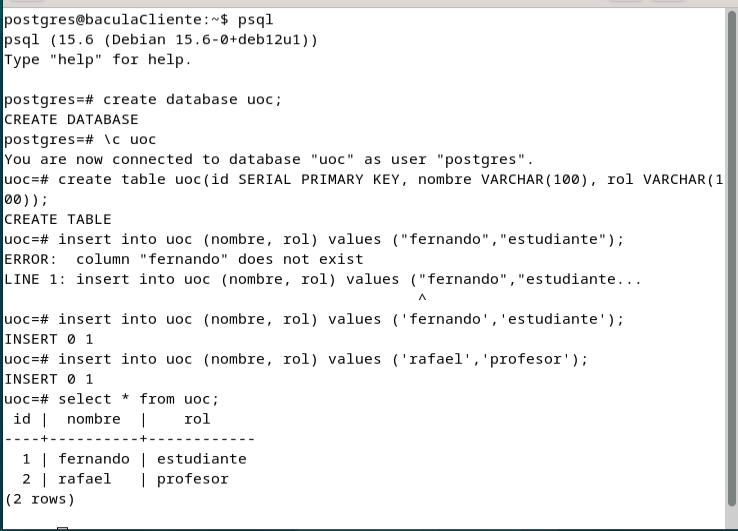
\includegraphics[width=0.5\linewidth]{instalacionBacula/postgrestCrearTabla.png}
    \caption{Creación y población de la tabla \textit{uoc} en PostgreSQL mostrando los comandos ejecutados y sus resultados.}
\end{figure}



\subsection{Configuración de Bacula en Debian}

\textbf{Configuración del Firewall}
\medskip

Primero, es necesario añadir las reglas al firewall para permitir el tráfico en los puertos utilizados por los componentes de Bacula. Los puertos son 9101 para el Director, 9102 para el File Daemon y 9103 para el Storage Daemon. Usamos los siguientes comandos:
\begin{verbatim}
sudo ufw allow 9101/tcp
sudo ufw allow 9102/tcp
sudo ufw allow 9103/tcp
\end{verbatim}

\begin{figure}[H]
    \centering
    \includegraphics[width=0.5\linewidth]{instalacionBacula/puertosBaCULAufw.png}
    \caption{Adición de reglas al firewall para Bacula}
\end{figure}

\textbf{Acceso a los Repositorios de Bacula}\medskip

Para instalar Bacula, primero debemos tener acceso a los repositorios. Es necesario registrarse en la página oficial \url{https://www.bacula.org/} para acceder a los repositorios de Bacula.

\begin{figure}[H]
    \centering
    \includegraphics[width=0.5\linewidth]{instalacionBacula/registroBacula.png}
    \caption{Página de registro para acceso a repositorios de Bacula}
\end{figure}

\textbf{Descarga e Instalación de Bacula}\medskip

Una vez registrados, accedemos a la sección de binarios y seleccionamos la última versión disponible para nuestro sistema.

\begin{figure}[H]
    \centering
    \includegraphics[width=0.5\linewidth]{instalacionBacula/baculapackages.png}
    \caption{Acceso a los binarios de Bacula}
\end{figure}

\textbf{Añadir Clave de Verificación y Repositorio}\medskip

Añadimos la clave de verificación y el repositorio de Bacula a nuestro sistema con los siguientes comandos:
\begin{verbatim}
wget https://bacula.org/downloads/Bacula-4096-Distribution-Verification-key.asc
apt-key add Bacula-4096-Distribution-Verification-key.asc
\end{verbatim}

\begin{figure}[H]
    \centering
    \includegraphics[width=0.5\linewidth]{instalacionBacula/baculaSignature.png}
    \caption{Añadiendo la clave de verificación de Bacula}
\end{figure}

\begin{figure}[H]
    \centering
    \includegraphics[width=0.5\linewidth]{instalacionBacula/baculaRepositorio.png}
    \caption{Añadiendo el repositorio de Bacula a sources.list}
\end{figure}

\textbf{MySQl vs PostgreSQL}
\medskip

Antes de seguir un aspecto importante es que base de datos para el catalogo elegir.


Cuando configuras Bacula para gestionar copias de seguridad, elegir entre MySQL y PostgreSQL para su servicio de catálogo puede depender de varias consideraciones técnicas y de licencia. A continuación, se presenta una comparación detallada:



\begin{table}[H]
    \centering
    \small
    \begin{tabularx}{\textwidth}{>{\centering\arraybackslash}p{0.15\textwidth}>{\centering\arraybackslash}p{0.4\textwidth}>{\centering\arraybackslash}X} 
        \hline
        \thead{Aspecto} & \thead{MySQL} & \thead{PostgreSQL} \\
        \hline
        Licencia & GNU GPL, que es más restrictiva en términos de obligaciones de compartir cambios & BSD, más permisiva y flexible para el uso en productos derivados sin compartir el código.\\
        Madurez & Muy maduro y ampliamente adoptado en aplicaciones web y de empresa. & Extremadamente maduro, con un enfoque en características avanzadas y conformidad con SQL.\\
        Desempeño & Generalmente más rápido en operaciones de lectura y carga de trabajo menos complejas. & Excelente en transacciones complejas y operaciones concurrentes de alta integridad.\\
        Características & 	Orientado al rendimiento con características de usabilidad fácil. &Soporta un conjunto más amplio de características SQL, funciones avanzadas y tipos de datos. \\
        Soporte de Datos	& Bueno para manejar grandes volúmenes de datos en sitios menos complejos. & Mejor para manejar complejidades en grandes bases de datos y con requerimientos estrictos. \\
        Seguridad y Confiabilidad & Confiabilidad alta, pero PostgreSQL tiene una reputación superior en robustez y seguridad. & Considerado muy robusto y seguro, con soporte extenso para políticas de seguridad detalladas.\\
        Facilidad de Configuración & Relativamente fácil de configurar y popular en la comunidad con muchos recursos disponibles. & Requiere más configuración inicial pero es altamente personalizable.\\
        \bottomrule
    \end{tabularx}
    \caption{Comparación entre Postgresql y MySQL para el catálogo de bacula.}
\end{table}




Recomendaciones para usar MySQL o PostgreSQL con Bacula:

\begin{itemize}
    \item MySQL: Ideal para entornos donde la velocidad y la simplicidad son prioritarias. Su licencia GPL puede ser adecuada si el proyecto también se distribuirá bajo GPL o cuando la licencia no representa un problema.
    \item PostgreSQL: La mejor opción si se requiere un sistema de gestión de base de datos robusto, con características avanzadas y mejor conformidad con SQL. Su licencia BSD es favorable para incorporar Bacula en productos que no desean estar ligados a las restricciones de GPL.
\end{itemize}



\textbf{Instalación de Bacula con PostgreSQL}\medskip

Seleccionamos PostgreSQL como la base de datos para el catálogo de Bacula. Instalamos la base de datos y Bacula con los siguientes comandos:
\begin{verbatim}
apt-get install dbconfig-common postgresql
apt-get install bacula-postgresql
\end{verbatim}

\begin{figure}[H]
    \centering
    \includegraphics[width=0.5\linewidth]{instalacionBacula/baculapostgesql.png}
    \caption{Instalación de Bacula con soporte para PostgreSQL}
\end{figure}

Configuramos Bacula para usar PostgreSQL durante el proceso de instalación:

\begin{figure}[H]
    \centering
    \includegraphics[width=0.5\linewidth]{instalacionBacula/configbaculapostgre.png}
    \caption{Configuración de Bacula con PostgreSQL}
\end{figure}

\textbf{Verificación de la Instalación}\medskip

Finalmente, verificamos que Bacula ha sido instalado correctamente y que todos los componentes necesarios están presentes.

\begin{figure}[H]
    \centering
    \includegraphics[width=0.5\linewidth]{instalacionBacula/baculadir.png}
    \caption{Verificación de la instalación de Bacula}
\end{figure}

Añadimos al PATH los scripts de Bacula para facilitar la ejecución de comandos:
\begin{verbatim}
export PATH=$PATH:/opt/bacula/bin
\end{verbatim}
        

\subsection{Webmin}  

Webmin es una herramienta de administración de sistemas basada en la web muy popular para sistemas Unix-like, que incluye soporte para configurar y administrar varios servicios, entre ellos Bacula. Usar Webmin para administrar Bacula puede proporcionar varios beneficios, especialmente en términos de accesibilidad y facilidad de uso. A continuación, se detallan las razones para usar Webmin:

\begin{enumerate}
    \item \textbf{Accesibilidad}: Como interfaz basada en la web, Webmin permite a los administradores acceder a la configuración de Bacula desde cualquier lugar, solo necesitas un navegador web.
    \item \textbf{Usabilidad}: Webmin ofrece una interfaz de usuario gráfica intuitiva, lo que hace que sea más fácil para los usuarios que no están familiarizados con la línea de comandos.
    \item \textbf{Flexibilidad}: Permite gestionar no solo Bacula, sino también otros aspectos del sistema, lo que lo hace útil para administradores que desean una herramienta única para múltiples tareas.
    \item \textbf{Configuración simplificada}: Proporciona módulos que simplifican la configuración de las complejas opciones de Bacula, reduciendo el riesgo de errores.
    \item \textbf{Comunidad y soporte}: Tiene una gran base de usuarios y una comunidad activa que puede ofrecer soporte y consejos.
\end{enumerate}

Además webmin puede ser útil en la lucha contra el ransomware:
\begin{enumerate}
    \item \textbf{Actualizaciones del Sistema}: Webmin puede configurar y manejar actualizaciones automáticas para el sistema operativo y el software instalado, lo cual es crucial para protegerse contra vulnerabilidades conocidas que podrían ser explotadas por ransomware.
    \item \textbf{Gestión de Backups}: A través del módulo de Bacula u otros módulos de backup como el módulo de rsync, Webmin puede configurar políticas de backups regulares y seguras, esencial para la recuperación de datos en caso de un ataque de ransomware.
    \item \textbf{Control de Acceso y Seguridad}: Webmin permite configurar políticas de seguridad, como la gestión de permisos de usuarios, el uso de contraseñas seguras, y configuraciones de firewall. Establecer un control de acceso estricto puede ayudar a prevenir accesos no autorizados que podrían resultar en un cifrado malicioso de datos.
    \item \textbf{Monitoreo y Alertas}: Webmin proporciona módulos para el monitoreo del sistema que pueden ser configurados para alertar a los administradores sobre actividad sospechosa o no autorizada, un componente crucial en la detección temprana de ataques de ransomware u otras infracciones de seguridad.
    \item \textbf{Configuración de Servidores de Correo}: Configurar correctamente los servidores de correo para filtrar spam y mensajes maliciosos puede reducir el riesgo de phishing, que es uno de los vectores de ataque más comunes para la distribución de ransomware.
\end{enumerate}

Otras herramientas graficas comparadas con webmin:

\begin{table}[H]
    \centering
    \small
    \begin{tabularx}{\textwidth}{>{\centering\arraybackslash}p{0.2\textwidth}>{\centering\arraybackslash}p{0.24\textwidth}>{\centering\arraybackslash}p{0.24\textwidth}>{\centering\arraybackslash}X} 
        \hline
        \thead{Interfaz} & \thead{Webmin} & \thead{Bacula Web} & \thead{BAT} \\
        \hline
        Tipo de Interfaz &Basada en la web & Basada en la web & Aplicación de escritorio\\
        Accesibilidad	 & Acceso remoto a través del navegador web & Acceso remoto a través del navegador web & Local o remoto mediante X11 forwarding\\
        Configuración & Configuración simplificada mediante módulos GUI & Configuración y monitoreo visual de trabajos de backup &Gestión detallada de configuraciones de Bacula\\
        Monitoreo & Monitoreo básico de tareas y estado del sistema & Monitoreo avanzado de trabajos, incluyendo reportes & Monitoreo detallado y gestión de trabajos y dispositivos \\
        Integración del Sistema	&Alta, gestiona otros servicios del sistema & Específica para Bacula & Específica para Bacula \\
        Facilidad de Uso & Interfaz intuitiva y fácil de usar para administradores & Requiere algo de familiaridad con Bacula & Requiere conocimiento avanzado de Bacula\\
        Soporte y Documentación & Amplia documentación y soporte comunitario & Documentación limitada, soporte comunitario & Documentación técnica detallada, soporte limitado\\
        \bottomrule
    \end{tabularx}
    \caption{Comparación entre webmin y otras herramientas gráficas de bacula.}
\end{table}


\textbf{Instalación de Apache}
\medskip

Comenzamos por instalar Apache, que es necesario para Webmin.
\begin{verbatim}
apt install apache2
\end{verbatim}

\begin{figure}[H]
    \centering
    \includegraphics[width=0.5\linewidth]{instalacionBacula/apache2.png}
    \caption{Instalación de Apache2}
\end{figure}

\textbf{Configuración del Firewall}
\medskip

Agregamos las reglas necesarias en el firewall para permitir el tráfico HTTP y HTTPS.
\begin{verbatim}
sudo ufw allow 80/tcp
sudo ufw allow 443/tcp
\end{verbatim}

\begin{figure}[H]
    \centering
    \includegraphics[width=0.5\linewidth]{instalacionBacula/htpsFirewall.png}
    \caption{Añadiendo reglas de HTTP y HTTPS al firewall}
\end{figure}

\textbf{Instalación de Webmin}
\medskip

Procedemos a descargar y ejecutar el script para configurar los repositorios de Webmin.
\begin{verbatim}
curl -o setup-repos.sh https://raw.githubusercontent.com/webmin/
webmin/master/setup-repos.sh sh setup-repos.sh
\end{verbatim}

\begin{figure}[H]
    \centering
    \includegraphics[width=0.5\linewidth]{instalacionBacula/CURLwebmin.png}
    \caption{Descargando y ejecutando el script de configuración de Webmin}
\end{figure}

Instalamos Webmin utilizando el gestor de paquetes apt.
\begin{verbatim}
apt-get install webmin --install-recommends
\end{verbatim}

\begin{figure}[H]
    \centering
    \includegraphics[width=0.5\linewidth]{instalacionBacula/instalWebminn.png}
    \caption{Instalación de Webmin}
\end{figure}

\textbf{Configuración del Puerto en el Firewall}
\medskip

Añadimos la regla en el firewall para permitir el tráfico en el puerto 10000, usado por Webmin.
\begin{verbatim}
sudo ufw allow 10000/tcp
\end{verbatim}

\begin{figure}[H]
    \centering
    \includegraphics[width=0.5\linewidth]{instalacionBacula/puerto10000.png}
    \caption{Añadiendo el puerto de Webmin al firewall}
\end{figure}

\textbf{Acceso a la Interfaz de Webmin}
\medskip

Ahora podemos acceder a la interfaz de Webmin mediante un navegador web utilizando la dirección IP del servidor y el puerto configurado.

\begin{figure}[H]
    \centering
    \includegraphics[width=0.5\linewidth]{instalacionBacula/webmin.png}
    \caption{Interfaz de acceso a Webmin}
\end{figure}

\textbf{Configuración del Módulo Bacula en Webmin}
\medskip

Configuramos el módulo Bacula en Webmin añadiendo las rutas necesarias para los comandos de Bacula.
% poner enumerate
\begin{verbatim}
Bacula configuration directory: /opt/bacula/etc
Full path to bextract command: /opt/bacula/bin/bextract
Full path to bls command: /opt/bacula/bin/bls
Full path to btape command: /opt/bacula/bin/btape
\end{verbatim}

\begin{figure}[H]
    \centering
    \includegraphics[width=0.5\linewidth]{instalacionBacula/pathwebmin.png}
    \caption{Configuración de los comandos de Bacula en Webmin}
\end{figure}

\textbf{Configuración de PostgreSQL para Bacula}\medskip

Si es necesario, ajustamos la configuración de PostgreSQL para permitir la autenticación del usuario de Bacula.
\begin{verbatim}
# TYPE  DATABASE        USER            ADDRESS                 METHOD
local   all             all                                     md5
\end{verbatim}

\begin{figure}[H]
    \centering
    \includegraphics[width=0.5\linewidth]{instalacionBacula/md5postgesql.png}
    \caption{Configuración de PostgreSQL para Bacula}
\end{figure}

Reiniciamos el servicio de PostgreSQL para aplicar los cambios.
\begin{verbatim}
systemctl restart postgresql
\end{verbatim}


\subsection{Configuración del Almacenamiento en Bacula}

Primero, creamos un directorio para almacenar los respaldos y asignamos los permisos adecuados para que Bacula pueda gestionar los archivos.

\begin{figure}[H]
    \centering
    \includegraphics[width=0.5\linewidth]{instalacionBacula/mkdirbackups.png}
    \caption{Creación del directorio de respaldos en el servidor Bacula}
\end{figure}

En Webmin, navegamos a la configuración de dispositivos de almacenamiento de Bacula para agregar un nuevo dispositivo que apunte al directorio que acabamos de crear.

\begin{figure}[H]
    \centering
    \includegraphics[width=0.5\linewidth]{instalacionBacula/STO.png}
    \caption{Interfaz de configuración de dispositivos de almacenamiento en Webmin}
\end{figure}

Agregamos un nuevo dispositivo de almacenamiento local en Webmin con los siguientes detalles \textbf{Nombre del dispositivo de almacenamiento:} localBackups; \textbf{Directorio o archivo del dispositivo:} /opt/bacula/backups; \textbf{Nombre del tipo de medio:} localBackups.



\begin{minipage}[t]{0.45\textwidth}
    \vspace{0pt} % Alinea la parte superior de la minipágina con lo que esté al lado
    \begin{figure}[H]
        \centering
        \includegraphics[width=0.95\linewidth]{instalacionBacula/NSD.png}
        \caption{Creación de un nuevo dispositivo de almacenamiento en Webmin}
    \end{figure}    
    \end{minipage}%
    \hfill % Añade espacio entre las dos minipáginas si es necesario
    \begin{minipage}[t]{0.45\textwidth}
    \vspace{0pt} % Alinea la parte superior de la minipágina con lo que esté al lado
    \centering % Centra el contenido de la minipágina
        \begin{figure}[H]
            \centering
            \includegraphics[width=0.95\linewidth]{instalacionBacula/localbac.png}
            \caption{Detalles del nuevo dispositivo de almacenamiento creado en Webmin}
        \end{figure}
    \end{minipage}
    
\medskip



%añadir opciones


Procedemos a configurar el daemon de almacenamiento para manejar las solicitudes de almacenamiento de datos.

\begin{figure}[H]
    \centering
    \includegraphics[width=0.5\linewidth]{instalacionBacula/stdeamon.png}
    \caption{Configuración inicial del daemon de almacenamiento en Webmin}
\end{figure}

Añadimos un nuevo daemon de almacenamiento especificando la IP del servidor y el puerto que Bacula utilizará para la comunicación. Esto facilita la gestión y evita la necesidad de configurar nombres de host o DNS en entornos sin estas facilidades.

\begin{figure}[H]
    \centering
    \includegraphics[width=0.5\linewidth]{instalacionBacula/newsd.png}
    \caption{Añadiendo un nuevo daemon de almacenamiento en Webmin}
\end{figure}

Finalmente, configuramos y creamos un pool de volúmenes donde Bacula almacenará los backups. Especificamos el nombre del pool, el tipo de pool, y configuramos opciones como el periodo de retención y la capacidad máxima de los volúmenes.



\begin{minipage}[t]{0.45\textwidth}
    \vspace{0pt} % Alinea la parte superior de la minipágina con lo que esté al lado
    \begin{figure}[H]
        \centering
        \includegraphics[width=0.95\linewidth]{instalacionBacula/pollv.png}
        \caption{Pool de volúmenes en Webmin}
    \end{figure} 
    \end{minipage}%
    \hfill % Añade espacio entre las dos minipáginas si es necesario
    \begin{minipage}[t]{0.45\textwidth}
    \vspace{0pt} % Alinea la parte superior de la minipágina con lo que esté al lado
    \centering % Centra el contenido de la minipágina
    \begin{figure}[H]
        \centering
        \includegraphics[width=0.95\linewidth]{instalacionBacula/pool22.png}
        \caption{Creación de un nuevo pool de volúmenes en Webmin}
    \end{figure}
    \end{minipage}
    
\medskip






Ahora para  configurar el volumen:
\begin{figure}[H]
    \centering
    \includegraphics[width=0.5\linewidth]{instalacionBacula/createVolumePool.png}
    \caption{Configuración de detalles del pool de volúmenes en Webmin}
\end{figure}
\subsection{Instalación del Cliente Bacula en Linux}

\textbf{Configuración del Firewall}
\medskip

Primero, añadimos la regla necesaria al firewall para permitir la comunicación en el puerto utilizado por el File Daemon de Bacula, que es el 9102/tcp.

\begin{figure}[H]
    \centering
    \includegraphics[width=0.5\linewidth]{instalacionBacula/9102alfirewall.png}
    \caption{Adición del puerto 9102 al firewall para permitir la comunicación del File Daemon}
\end{figure}

\textbf{Instalación del Cliente Bacula}
\medskip

Procedemos a instalar el cliente Bacula en el sistema. Este proceso instala todos los componentes necesarios para que el cliente pueda comunicarse con el Director de Bacula.

\begin{verbatim}
apt install bacula-client
\end{verbatim}

A continuación, verificamos que la instalación se ha completado correctamente y que el servicio está activo y ejecutándose.

\begin{figure}[H]
    \centering
    \includegraphics[width=0.5\linewidth]{instalacionBacula/baculaClienteinstalacion2.png}
    \caption{Confirmación de la instalación y estado del servicio Bacula File Daemon}
\end{figure}

\textbf{Configuración del File Daemon}
\medskip

Editamos el archivo de configuración del File Daemon para establecer la conexión con el Director de Bacula. Aquí especificamos el nombre del Director y la contraseña que permite una conexión segura entre el cliente y el servidor.

\begin{verbatim}
nano /opt/bacula/etc/bacula-fd.conf
\end{verbatim}

Añadimos la configuración del Director, especificando su nombre y contraseña correspondiente. Este paso es crucial para la autenticación y la correcta comunicación entre el cliente y el servidor.

\begin{figure}[H]
    \centering
    \includegraphics[width=0.5\linewidth]{instalacionBacula/baculaFDcongf.png}
    \caption{Configuración del archivo bacula-fd.conf con detalles del Director}
\end{figure}

Estos pasos garantizan que el cliente Bacula esté correctamente configurado y pueda comunicarse de manera segura con el servidor Bacula Director, facilitando así la gestión centralizada de los respaldos.

\subsection{Funcionamiento del Plugin bpipe de Bacula}

El plugin bpipe de Bacula proporciona una funcionalidad flexible y poderosa para ejecutar comandos externos y gestionar su entrada y salida dentro de las tareas de backup y restore. Esto permite a los administradores integrar prácticamente cualquier software o script que pueda generar o aceptar datos desde la línea de comandos, directamente en el proceso de backup o restauración.

\textbf{Propósito del Plugin}

El propósito principal del plugin bpipe es permitir que Bacula pueda incluir datos que no están directamente almacenados en sistemas de archivos, tales como bases de datos, información de configuración en vivo, o cualquier otra información accesible a través de comandos de shell. El plugin bpipe se utiliza tanto para backups como para restauraciones, manipulando datos en vuelo sin necesidad de almacenarlos temporalmente en el disco.

\textbf{Funcionamiento General}

Cuando se configura un job de Bacula que utiliza el plugin bpipe, se especifican dos comandos principales:

\begin{itemize}
    \item \textbf{Comando para Backup:} Este comando es ejecutado por Bacula al realizar un backup. El plugin bpipe redirige la salida de este comando (datos generados por el comando) directamente hacia el destino del backup. Esto es útil para capturar datos en tiempo real, como un dump de base de datos.
    
    \item \textbf{Comando para Restore:} En el caso de una restauración, el plugin bpipe ejecuta este comando y le proporciona los datos que necesitan ser restaurados. Esto permite que el comando procese los datos y los restablezca en su destino original o en uno nuevo especificado.
\end{itemize}

\textbf{Parámetros del Plugin bpipe}

Para configurar correctamente el plugin bpipe, se deben especificar varios parámetros en el archivo de configuración del Job de Bacula. Estos parámetros incluyen:

\begin{itemize}
    \item \textbf{Nombre del Plugin:} Generalmente se define como \textit{bpipe} para indicar que el job utilizará este plugin.
    \item \textbf{FileSet:} Se especifica en el conjunto de archivos, donde el nombre del archivo virtual en Bacula será el manejador para los datos de entrada/salida del comando.
    \item \textbf{Comando de Backup:} El comando que Bacula debe ejecutar para obtener los datos a respaldar.
    \item \textbf{Comando de Restore:} El comando que Bacula debe ejecutar para restaurar los datos desde el backup.
\end{itemize}

Estos parámetros se definen en la configuración del \textit{FileSet} y son cruciales para el correcto funcionamiento del plugin. La capacidad de ejecutar comandos personalizados para manejar datos específicos ofrece una flexibilidad considerable, permitiendo a Bacula adaptarse a entornos complejos y a necesidades específicas de backup y restauración.

\textbf{Consideraciones de Seguridad}

Dado que el plugin bpipe puede ejecutar cualquier comando, es vital asegurarse de que los comandos utilizados son seguros y provienen de fuentes confiables. Los comandos deben ser cuidadosamente revisados y probados para evitar la ejecución de operaciones no deseadas o maliciosas.

%%%%%%%%%%%%%primero de todo descargamos una imagen de debian, para ello vamos a la web de debian https://www.debian.org/distrib/ y elegimos la iso que mejor se adapte a lo que necesitamos, yo en mi caso elegi el instalador a traver de internet
\begin{figure}[H]
    \centering
    \includegraphics[width=0.5\linewidth]{instalacionBacula/debianPaginaWeb.png}
    \caption{Enter Caption}
\end{figure}
En virtual box añadimos una nueva maquina virtual, le ponemos un nombre y seleccionamos la iso de debian
\begin{figure}[H]
    \centering
    \includegraphics[width=0.5\linewidth]{instalacionBacula/vbDebian.png}
    \caption{Enter Caption}
\end{figure}


Ahora configuramos el usuario y la contranseña de la maquina:

\begin{figure}[H]
    \centering
    \includegraphics[width=0.5\linewidth]{instalacionBacula/instalación desatendida del SO.png}
    \caption{Enter Caption}
\end{figure}

Configuramos el hardware, debian no es un sistema operativo muy pesado y no necesita muchos recursos para que funcione de forma fluida, asique no es necesario darle mucha memoria base y procesadores:
\begin{figure}[H]
    \centering
    \includegraphics[width=0.5\linewidth]{instalacionBacula/vbhardware.png}
    \caption{Enter Caption}
\end{figure}

Ahora necesitamos asignarle el almacenamiento para ello creamos un disco duro virtual, y le asignamos 50 GB
\begin{figure}[H]
    \centering
    \includegraphics[width=0.5\linewidth]{instalacionBacula/vbDisco.png}
    \caption{Enter Caption}
\end{figure}

Ahora instalamos y dejamos que el instalador haga su trabajo.

Una vez instalado realizamos en la consola un upgrade y un update del sistema:

\begin{figure}[H]
    \centering
    \includegraphics[width=0.5\linewidth]{instalacionBacula/Update y upgrade.png}
    \caption{Enter Caption}
\end{figure}

Finalmente en la configuracion en virtual box cambiamos la red de nat a adaptador puente:

\begin{figure}[H]
    \centering
    \includegraphics[width=0.5\linewidth]{instalacionBacula/NatAdaptadorPuente.png}
    \caption{Enter Caption}
\end{figure}



%%%%%%%%%%%%%%%%%%%%%%%%%%%%%%%%%%%%%%%%%%%%%%%%
---------------------------------------------
Primero necesitamos añadir los puertos de bacula al firewall
puertos 9101 director 9102 file deamon 9103 storage deamon
para ello usamos los comandos:

sudo ufw allow 9101/tcp
sudo ufw allow 9102/tcp
sudo ufw allow 9103/tcp



\begin{figure}[H]
    \centering
    \includegraphics[width=0.5\linewidth]{instalacionBacula/puertosBaCULAufw.png}
    \caption{Enter Caption}
\end{figure}

A continuacion necesitamos tener acceso a los repositorios de bacula, desafortunadamente tienes que estar registrado en su pagina  https://www.bacula.org/ para obtenerlos

\begin{figure}[H]
    \centering
    \includegraphics[width=0.5\linewidth]{instalacionBacula/registroBacula.png}
    \caption{Enter Caption}
\end{figure}


Una vez registrados ya podemos acceder a los binarios, para ello vamos a 
debs -> ultima version 15.0.2 -> dist -> bookworm-> main-binary amd -> install


\begin{figure}[H]
    \centering
    \includegraphics[width=0.5\linewidth]{instalacionBacula/baculapackages.png}
    \caption{Enter Caption}
\end{figure}

Añadimos la clave de verificacion distribucion con los comandos:
  wget https://bacula.org/downloads/Bacula-4096-Distribution-Verification-key.asc
  apt-key add Bacula-4096-Distribution-Verification-key.asc
  

  

\begin{figure}[H]
    \centering
    \includegraphics[width=0.5\linewidth]{instalacionBacula/baculaSignature.png}
    \caption{Enter Caption}
\end{figure}

Y los repositorios a sources.list :

\begin{figure}[H]
    \centering
    \includegraphics[width=0.5\linewidth]{instalacionBacula/baculaRepositorio.png}
    \caption{Enter Caption}
\end{figure}

Antes de seguir un aspecto importante es que base de datos para el catalogo elegir.
Cuando configuras Bacula para gestionar copias de seguridad, elegir entre MySQL y PostgreSQL para su servicio de catálogo puede depender de varias consideraciones técnicas y de licencia. A continuación, se presenta una comparación detallada:


\begin{table}
    \centering
    \begin{tabular}{ccc}
        Aspecto & MySQL & PostgreSQL\\
        Licencia & GNU GPL, que es más restrictiva en términos de obligaciones de compartir cambios & BSD, más permisiva y flexible para el uso en productos derivados sin compartir el código.\\
        Madurez & Muy maduro y ampliamente adoptado en aplicaciones web y de empresa. & Extremadamente maduro, con un enfoque en características avanzadas y conformidad con SQL.\\
        Desempeño & Generalmente más rápido en operaciones de lectura y carga de trabajo menos complejas. & Excelente en transacciones complejas y operaciones concurrentes de alta integridad.\\
        Características & 	Orientado al rendimiento con características de usabilidad fácil. &Soporta un conjunto más amplio de características SQL, funciones avanzadas y tipos de datos. \\
        Soporte de Datos	& Bueno para manejar grandes volúmenes de datos en sitios menos complejos. & Mejor para manejar complejidades en grandes bases de datos y con requerimientos estrictos. \\
        Seguridad y Confiabilidad & Confiabilidad alta, pero PostgreSQL tiene una reputación superior en robustez y seguridad. & Considerado muy robusto y seguro, con soporte extenso para políticas de seguridad detalladas.\\
        Facilidad de Configuración & Relativamente fácil de configurar y popular en la comunidad con muchos recursos disponibles. & Requiere más configuración inicial pero es altamente personalizable.\\
    \end{tabular}
    \caption{Caption}
\end{table}


Recomendaciones para usar MySQL o PostgreSQL con Bacula:
MySQL: Ideal para entornos donde la velocidad y la simplicidad son prioritarias. Su licencia GPL puede ser adecuada si el proyecto también se distribuirá bajo GPL o cuando la licencia no representa un problema.

PostgreSQL: La mejor opción si se requiere un sistema de gestión de base de datos robusto, con características avanzadas y mejor conformidad con SQL. Su licencia BSD es favorable para incorporar Bacula en productos que no desean estar ligados a las restricciones de GPL.

Yo me decline por postgres por tanto instalamos la base de datos para el catalogo con apt-get install dbconfig-common postgresql y instalmos bacula con postgres mediante apt-get install bacula-postgresql.
\begin{figure}[H]
    \centering
    \includegraphics[width=0.5\linewidth]{instalacionBacula/baculapostgesql.png}
    \caption{Enter Caption}
\end{figure}


configuramos baccula con postgresql
\begin{figure}[H]
    \centering
    \includegraphics[width=0.5\linewidth]{instalacionBacula/configbaculapostgre.png}
    \caption{Enter Caption}
\end{figure}

Y comprobamos que se instalo correctamente:
\begin{figure}[H]
    \centering
    \includegraphics[width=0.5\linewidth]{instalacionBacula/baculadir.png}
    \caption{Enter Caption}
\end{figure}

Y añadimos al path los scripts de bacula con
export PATH=\$PATH:/opt/bacula/bin


\newpage
%%%%%%%%%%%%%%%%%%%%%%%%%%%%%%%%%%%%%%%%%%%%%%%%%%%
----------------------------------

instalar webmin


primero instalamos apache:

\begin{figure}[H]
    \centering
    \includegraphics[width=0.5\linewidth]{instalacionBacula/apache2.png}
    \caption{Enter Caption}
\end{figure}


añadimos http y https al firewall

sudo ufw allow 80/tcp
sudo ufw allow 443/tcp


\begin{figure}[H]
    \centering
    \includegraphics[width=0.5\linewidth]{instalacionBacula/htpsFirewall.png}
    \caption{Enter Caption}
\end{figure}



PARA INSTALAR  webmin 
curl -o setup-repos.sh https://raw.githubusercontent.com/webmin/webmin/master/setup-repos.sh
sh setup-repos.sh

\begin{figure}[H]
    \centering
    \includegraphics[width=0.5\linewidth]{instalacionBacula/CURLwebmin.png}
    \caption{Enter Caption}
\end{figure}


apt-get install webmin --install-recommends


\begin{figure}[H]
    \centering
    \includegraphics[width=0.5\linewidth]{instalacionBacula/instalWebminn.png}
    \caption{Enter Caption}
\end{figure}


y añadimos el puerto 10000 al firewal
\begin{figure}[H]
    \centering
    \includegraphics[width=0.5\linewidth]{instalacionBacula/puerto10000.png}
    \caption{Enter Caption}
\end{figure}


Y ahora ya podemos acceder la consola de webmin en el navegador:

\begin{figure}[H]
    \centering
    \includegraphics[width=0.5\linewidth]{instalacionBacula/webmin.png}
    \caption{Enter Caption}
\end{figure}


ahora podemos configurar el modulo de bacula en webmin 
añadimos los directorios de bacula a webmin

Bacula configuration directory
/opt/bacula/etc
Full path to bextract command
/opt/bacula/bin/bextract
Full path to bls command
/opt/bacula/bin/bls
Full path to btape command
/opt/bacula/bin/btape

\begin{figure}[H]
    \centering
    \includegraphics[width=0.5\linewidth]{instalacionBacula/pathwebmin.png}
    \caption{Enter Caption}
\end{figure}


si diese error habria que en el archivo de configuracion pg\_hba.conf de postgesql/15/main y darle/cambiarle permisos de autentificacion a nuestro usuario de bacula para ello

\# TYPE  DATABASE        USER            ADDRESS                 METHOD
local   all             all                                     md5

\begin{figure}[H]
    \centering
    \includegraphics[width=0.5\linewidth]{instalacionBacula/md5postgesql.png}
    \caption{Enter Caption}
\end{figure}

guardamos y reiniciamos el servicio de postgresql
systemctl restart postgresql

%%%%%%%%%%%%%%%%%%%%%%%%%%%%%%%%
-------------------------

configuracion del almacenamiento local

creamos un directorio para almacenamiento 
con mkdir backups

y le damos propiedad a bacula sobre esa direccion con 

\begin{figure}[H]
    \centering
    \includegraphics[width=0.5\linewidth]{instalacionBacula/mkdirbackups.png}
    \caption{Enter Caption}
\end{figure}



\begin{figure}[H]
    \centering
    \includegraphics[width=0.5\linewidth]{instalacionBacula/STO.png}
    \caption{Enter Caption}
\end{figure}


NOS ENCONTRAMOS UNOS STORAGES DEVICES QUE VIENEN DEFAULT
PERO CREAMOS UNO NUEVO
\begin{figure}[H]
    \centering
    \includegraphics[width=0.5\linewidth]{instalacionBacula/NSD.png}
    \caption{Enter Caption}
\end{figure}

(explcar estos:)
Storage device name
    localBackups
Archive device or directory
    /otp/bacula/backups
Media type name
    localBackups

\begin{figure}[H]
    \centering
    \includegraphics[width=0.5\linewidth]{instalacionBacula/localbac.png}
    \caption{Enter Caption}
\end{figure}


en este directorio nos van a ver los archivos sueltos de los backups que van a ir tomando.

Van a ver un archivo donde en él va a estar de manera cifrada toda la información que ustedes vayan

respaldando con lo cual si alguien les ganar acceso al servidor local simplemente verían una cosa así.

Eso sería todo lo que vería en un archivo solo y nada de información.
configuramos en bacula el uso de almacenamiento local


ahora creamos un storage deamon
\begin{figure}[H]
    \centering
    \includegraphics[width=0.5\linewidth]{instalacionBacula/stdeamon.png}
    \caption{Enter Caption}
\end{figure}


añadimo un nuevo storage deamon
\begin{figure}[H]
    \centering
    \includegraphics[width=0.5\linewidth]{instalacionBacula/newsd.png}
    \caption{Enter Caption}
\end{figure}

si ponemos el nombre del servidor tenemos que enseñarle a todos los clientes que vamos a realizarles copias de seguridad que puedan resolver el servidor por nombre en nuestro caso como no tenemos un servidor de DNS vamos a poner acá la dirección IP del servidor de backup para ahorrarnos el trabajo de los clientes tener que andar editando el archivo hoost entonces vamos a poner directamente la IP del servidor 

Details of remote storage daemon
(habria que explicar estas opciones)
-Storage daemon name
StorageDeamon
-Bacula SD password
1234
-Hostname or IP address
192.168.1.114
-Bacula SD port
9103
-Storage device name

localBackups
 

-Media type name
localBackups
-Maximum concurrent jobs
20


\begin{figure}[H]
    \centering
    \includegraphics[width=0.5\linewidth]{instalacionBacula/storagedeamonWebmin.png}
    \caption{Enter Caption}
\end{figure}
para mejorar la seguridad de las copias de seguridad agregando certificados y habilitando las comunicaciones TLS.

Y ya tendriamos el storage deamon:
\begin{figure}[H]
    \centering
    \includegraphics[width=0.5\linewidth]{instalacionBacula/sdwebminaa.png}
    \caption{Enter Caption}
\end{figure}





por ultimo cremos nuestro propio pool de volumenes:

\begin{figure}[H]
    \centering
    \includegraphics[width=0.5\linewidth]{instalacionBacula/pollv.png}
    \caption{Enter Caption}
\end{figure}



\begin{figure}[H]
    \centering
    \includegraphics[width=0.5\linewidth]{instalacionBacula/pool22.png}
    \caption{Enter Caption}
\end{figure}

ahora para  configurar el volumen:
Details of backup volume pool

(abria que explcar estas opciones)
-Volume pool name
Pool1
-Volume pool type

Backup
-Maximum jobs per volume

  Unlimited 
 
  
-Volume retention period
    365 days
    
-Automatically recycle volumes?

  Yes 
 
  Default 
-Prune expired volumes?

  Yes 
 
 
  Default 
-Automatically label volumes prefix
Backup
-Maximum volume size 
3G

\begin{figure}
    \centering
    \includegraphics[width=0.5\linewidth]{instalacionBacula/createVolumePool.png}
    \caption{Enter Caption}
\end{figure}


Pueden ponerlo de 15 días de tres meses de un año.

Esto lo vamos a ir viendo más en detalle adelante cuando hablemos de estrategias de backup.

Y por último podemos ponerle un límite al tamaño que cada uno de esos archivos puede tener.

Vamos a ponerle 10 siglas cada uno de estos archivos donde vaya guardando los backups no puede exceder los 3 gigas.

Esto también es parte de una estrategia de backup.

Por el momento vamos a dejarlo así para que podamos hacer una práctica simple de backup y después lo

abordaremos cuando vemos estrategias.

%%%%%%%%%
------------------------------------- 
Instalar bacula client en Linux

añadimos el file demon baculhel puerto 9102 al firewall 
\begin{figure} [H]
    \centering
    \includegraphics[width=0.5\linewidth]{instalacionBacula/9102alfirewall.png}
    \caption{Enter Caption}
\end{figure}


al igual que antes añadimos los repositorios de bacula


ahora instalamos el cliente de bacula:
apt install bacula-client

y como vemos se instalo correctamente:

\begin{figure}[H]
    \centering
    \includegraphics[width=0.5\linewidth]{instalacionBacula/baculaClienteinstalacion2.png}
    \caption{Enter Caption}
\end{figure}

y editamos el archivo /opt/bacula/etc/bacula-fd.conf

\begin{figure}[H]
    \centering
    \includegraphics[width=0.5\linewidth]{instalacionBacula/baculaFDcongf.png}
    \caption{Enter Caption}
\end{figure}

%%%%%%%%%%%%%%
--------------------
realizar backup

necesitamos definir lo siguiente:

definir que es lo que vamos a respaldar
definir cuando lo vamos a respaldar
agregar a quien  vamos a respaldar
crear el  job 
y ejecutar el job




creamos un fileset en webmin

\begin{figure}[H]
    \centering
    \includegraphics[width=0.5\linewidth]{instalacionBacula/filesetwebmin.png}
    \caption{Enter Caption}
\end{figure}

hay dos fileset creados durante la instalacion

\begin{figure}[H]
    \centering
    \includegraphics[width=0.5\linewidth]{instalacionBacula/cpropiofileset.png}
    \caption{Enter Caption}
\end{figure}


 reutilizar el Falset en sus diferentes definiciones de Jobs o pueden crear un Falset por cada cliente.

Esto es decisión y gusto de cada uno.

Vamos a poner md5 de para que de esta manera se asegure de que lo que está copiando es una copia fiel

va a comparar las hash MD5 


File set name
ClienteDebian1Archivos
Files and directories to backup
/etc
/root
/home
File signature type
MD5

Files and directories to skip


Compression type

<Default compression level>
Limit backup to one filesystem?

  Yes 
 
  No 
 
  Default 


  \begin{figure}[H]
      \centering
      \includegraphics[width=0.5\linewidth]{instalacionBacula/createrfilesett.png}
      \caption{Enter Caption}
  \end{figure}


ahora creamos un schedule:
\begin{figure}[H]
    \centering
    \includegraphics[width=0.5\linewidth]{instalacionBacula/schedule.png}
    \caption{Enter Caption}
\end{figure}

hay ya 2 que vienen con el sistema:

Schedule name	Run levels and times
WeeklyCycle	Full 1st sun at 23:05 , Differential 2nd-5th sun at 23:05 , ...
WeeklyCycleAfterBackup	Full sun-sat at 23:10

pero vamos a crear uno nuevo

\begin{figure}[H]
    \centering
    \includegraphics[width=0.5\linewidth]{instalacionBacula/newBackupSchedules.png}
    \caption{Enter Caption}
\end{figure}

aqui nos da las tres opciones de backup, full, partial o diferencial, sobre que volumen hacerlo, y cada cuanto hacerlo:

\begin{figure}[H]
    \centering
    \includegraphics[width=0.5\linewidth]{instalacionBacula/editbuckupschedule.png}
    \caption{Enter Caption}
\end{figure}






ahora necesitamos selecionar a quien vamos a backupear
\begin{figure}[H]
    \centering
    \includegraphics[width=0.5\linewidth]{instalacionBacula/asdasdas.png}
    \caption{Enter Caption}
\end{figure}

de momento solo esta el propio server bacula que se autoagrega en la instalacion, añadimos un nuevo cliente:

\begin{figure}[H]
    \centering
    \includegraphics[width=0.5\linewidth]{instalacionBacula/addnewbuckupclient.png}
    \caption{Enter Caption}
\end{figure}


ahora necesitamos definir los Details of client to be backed up
estas opciones son:
-Client FD name
baculaCliente-fd
-Bacula FD password

-Hostname or IP address
192.168.1.116
-Bacula FD port
9102
-Catalog to use

MyCatalog
-Prune expired jobs and files?

  Yes 
 
  No 
 
  Default 
-Keep backup files for
1 months
-Keep backup jobs for
1 months


\begin{figure}[H]
    \centering
    \includegraphics[width=0.5\linewidth]{instalacionBacula/detalesclienteparabuckup.png}
    \caption{Enter Caption}
\end{figure}

ademas podemos añadir encriptacion tls


Ahora podemos crear y ejecutar un job:

\begin{figure}[H]
    \centering
    \includegraphics[width=0.5\linewidth]{instalacionBacula/createJOB.png}
    \caption{Enter Caption}
\end{figure}

aqui hay una serie de jobs que vienen por default:

Job name	Defaults?	Job type	Client to backup	File set to backup	Backup schedule
BackupCatalog	No	Default	Default	Catalog	WeeklyCycleAfterBackup
BackupClient1	No	Default	Default	Default	Default
DefaultJob	Yes	Backup	baculaServer-fd	Full Set	WeeklyCycle
RestoreFiles	No	Restore	baculaServer-fd	Full Set	Default

creamos uno nuevo

\begin{figure}[H]
    \centering
    \includegraphics[width=0.5\linewidth]{instalacionBacula/createnewjob.png}
    \caption{Enter Caption}
\end{figure}

y definimos los detalles del job:
\begin{figure}[H]
    \centering
    \includegraphics[width=0.5\linewidth]{instalacionBacula/Backupjobdetails.png}
    \caption{Enter Caption}
\end{figure}
estas opciones son:
-Backup job enabled?

  Yes 
 
  No 
-Default type

  Default definiton 
 
  Stand-alone job 
 
  Inherit defaults from 

  DefaultJob
-Job type

Backup
Backup level

Full

-Client to backup

baculaCliente-fd
-File set to backup

ClienteDebian1Archivos
-Backup on schedule

schedule1
-Destination storage device

StorageDeamon
-Volume pool

Pool1
-Destination for messages

Standard
-Backup priority

  Default 
 
  
tambien se pueden ejecutar comandos antes o despues del job en el cliente o el servidor



para ejecutar un job (de forma manual)

\begin{figure}[H]
    \centering
    \includegraphics[width=0.5\linewidth]{instalacionBacula/runbackupjonbb.png}
    \caption{Enter Caption}
\end{figure}

elegimos el job que queremos ejecutar y hacemos backup now
\begin{figure}[H]
    \centering
    \includegraphics[width=0.5\linewidth]{instalacionBacula/backupnoww.png}
    \caption{Enter Caption}
\end{figure}

y nos devuelve una salida como la siguiente:
\begin{figure}[H]
    \centering
    \includegraphics[width=0.5\linewidth]{instalacionBacula/salidajob1.png}
    \caption{Enter Caption}
\end{figure}

%%%%%%%%%%%%%%%%%%%%%%
---------------------------
Restore en linux cliente

para ello he creado 5 archivos txt y he obtenido el md5 sum de 2 y 3 que los voy a borrar:

\begin{figure}[H]
    \centering
    \includegraphics[width=0.5\linewidth]{instalacionBacula/5ARCHIVOS.png}
    \caption{Enter Caption}
\end{figure}

Primero hago el backup en bacula:
\begin{figure}[H]
    \centering
    \includegraphics[width=0.5\linewidth]{instalacionBacula/backup0002.png}
    \caption{Enter Caption}
\end{figure}

eliminamos los archivos 2 y 3:

\begin{figure}[H]
    \centering
    \includegraphics[width=0.5\linewidth]{instalacionBacula/rmArchivo23.png}
    \caption{Enter Caption}
\end{figure}

y ahora hacemos un restore backup:

\begin{figure}[H]
    \centering
    \includegraphics[width=0.5\linewidth]{instalacionBacula/resBackup.png}
    \caption{Enter Caption}
\end{figure}
Job to restore

estas opciones son:

-Files to restore
/home/archivo2.txt
/home/archivo3.txt
 
-Restore from storage device

StorageDeamon
-Restore to client or group

baculaCliente-fd (on 192.168.1.116)
-Restore to directory

  Default (/opt/bacula/archive/bacula-restores) 


  Other root directory 
 
/
-Wait for results?

  Yes 
 
  No 

\begin{figure}[H]
    \centering
    \includegraphics[width=0.5\linewidth]{instalacionBacula/restoresalidawebmin.png}
    \caption{Enter Caption}
\end{figure}

y como podemos ver se restauraron correctamente:
\begin{figure}[H]
    \centering
    \includegraphics[width=0.5\linewidth]{instalacionBacula/restoreSusc.png}
    \caption{Enter Caption}
\end{figure}

%%%%%%%%%%%%%%%%%%%%%%%%%%%%%%%%%%%%%%%%
----------------
Instalar bacula client en Windows



primero descargamos bacula, para ello vamos a su web- downloads - windows binaries

\begin{figure}[H]
    \centering
    \includegraphics[width=0.5\linewidth]{instalacionBacula/winbinaries.png}
    \caption{Enter Caption}
\end{figure}

Y descargamos la ultima version
\begin{figure}[H]
    \centering
    \includegraphics[width=0.5\linewidth]{instalacionBacula/downloadwinbinaries.png}
    \caption{Enter Caption}
\end{figure}

Iniciamos el instalador

\begin{figure}[H]
    \centering
    \includegraphics[width=0.5\linewidth]{instalacionBacula/instalador.png}
    \caption{Enter Caption}
\end{figure}

aceptamos acuerdo de licencia:
\begin{figure}[H]
    \centering
    \includegraphics[width=0.5\linewidth]{instalacionBacula/lecencia.png}
    \caption{Enter Caption}
\end{figure}

elegimos el tipo de instalcion, en mi caso custom

\begin{figure}[H]
    \centering
    \includegraphics[width=0.5\linewidth]{instalacionBacula/custom.png}
    \caption{Enter Caption}
\end{figure}

Como queremos instalar un cliente elegimos las caracteristicas de cliente:
\begin{figure}[H]
    \centering
    \includegraphics[width=0.5\linewidth]{instalacionBacula/clientecaracteristicas.png}
    \caption{Enter Caption}
\end{figure}


elegimos la ruta de instalacion:
\begin{figure}[H]
    \centering
    \includegraphics[width=0.5\linewidth]{instalacionBacula/rutawindebacula.png}
    \caption{Enter Caption}
\end{figure}

applicamos la configuracion
nombre: win-fd
puerto 9102
max job que es el numero de trabajos simultaneos 5
contraseña, una segura


\begin{figure}[H]
    \centering
    \includegraphics[width=0.5\linewidth]{instalacionBacula/configwinbaCULA.png}
    \caption{Enter Caption}
\end{figure}


tambien tenemos que poner la informacion del director: 
nombre baculaServer-dir
puerto 9101
contraseña
direccion 192.168.1.114

\begin{figure}[H]
    \centering
    \includegraphics[width=0.5\linewidth]{instalacionBacula/config2winbacula.png}
    \caption{Enter Caption}
\end{figure}

Intalamos y esperamos a que termine:

\begin{figure}[H]
    \centering
    \includegraphics[width=0.5\linewidth]{instalacionBacula/teminadoInstalarBaculawin.png}
    \caption{Enter Caption}
\end{figure}

Ahora en el firewall de windows- reglas de entrada- nueva regla
y añadimos bacula al firewall

\begin{figure}[H]
    \centering
    \includegraphics[width=0.5\linewidth]{instalacionBacula/firewallwindows.png}
    \caption{Enter Caption}
\end{figure}

Ahora necesitamos que el servicio interactue con el escritorio, para ello debemos permitirlo en services:

\begin{figure}
    \centering
    \includegraphics[width=0.5\linewidth]{instalacionBacula/permitirservicio.png}
    \caption{Enter Caption}
\end{figure}

%%%%%%%%%%%%%%%%%%%%%%%%%%%%%
-----------------------
Realizar backup windows

que vamos a backupear:

vamos a fileset
\begin{figure}[H]
    \centering
    \includegraphics[width=0.5\linewidth]{instalacionBacula/filesetwebmin.png}
    \caption{Enter Caption}
\end{figure}


creamos un fileset nuevo:

\begin{figure}[H]
    \centering
    \includegraphics[width=0.5\linewidth]{instalacionBacula/cpropiofileset.png}
    \caption{Enter Caption}
\end{figure}

elegimos las opciones que necesitemos:

Backup file set details
File set name
FileSetWin
Files and directories to backup
C:/Usuarios/yo/Documents
File signature type

None
Files and directories to skip
Compression type

<Default compression level>
Limit backup to one filesystem?

  Yes 
 
  No 
 
  Default 

\begin{figure}[H]
    \centering
    \includegraphics[width=0.5\linewidth]{instalacionBacula/filesetWindows.png}
    \caption{Enter Caption}
\end{figure}


ahora hay que definir cuando queremos hacer el backup
para ello habria que definirlo en backup schedule, 

\begin{figure}[H]
    \centering
    \includegraphics[width=0.5\linewidth]{instalacionBacula/schedule.png}
    \caption{Enter Caption}
\end{figure}

en mi caso voy a reutilizar el schedule de linux anteriormente creado


ahora hay que defir a quien le vamos a realizar el backup, para ello vamos a backup clients

\begin{figure}[H]
    \centering
    \includegraphics[width=0.5\linewidth]{instalacionBacula/asdasdas.png}
    \caption{Enter Caption}
\end{figure}

y añadimos el nuevo cliente windows

Details of client to be backed up
Client FD name
win-fd
Bacula FD password
1234
Hostname or IP address
192.168.1.112
Bacula FD port
9102
Catalog to use

MyCatalog
Prune expired jobs and files?

  Yes 
 
  No 
 
  Default 
Keep backup files for
1
 
months
Keep backup jobs for
1
 
months
\begin{figure}[H]
    \centering
    \includegraphics[width=0.5\linewidth]{instalacionBacula/createbackupclientwindows.png}
    \caption{Enter Caption}
\end{figure}


ahora creamos un backup job


Backup job details
Backup job name
WindowsJob
Backup job enabled?

  Yes 
 
  No 
Default type

  Default definiton 
 
  Stand-alone job 
 
  Inherit defaults from 

DefaultJob
Job type

Backup
Backup level

Full
Client to backup

win-fd
File set to backup

FileSetWin
Backup on schedule

schedule1
Destination storage device

StorageDeamon
Volume pool

Pool1
Destination for messages

Standard
Backup priority

  Default 
 
 \begin{figure}[H]
    \centering
    \includegraphics[width=0.5\linewidth]{instalacionBacula/createJOB.png}
    \caption{Enter Caption}
\end{figure}

 
ahora podemos hacer el backup:
\begin{figure}[H]
    \centering
    \includegraphics[width=0.5\linewidth]{instalacionBacula/backupWindows.png}
    \caption{Enter Caption}
\end{figure}


-----------------
realizar restore windows


primero he creado 3 archivos .txt
\begin{figure}[H]
    \centering
    \includegraphics[width=0.5\linewidth]{instalacionBacula/archivosWin.png}
    \caption{Enter Caption}
\end{figure}

Hacemos el backup:

\begin{figure}[H]
    \centering
    \includegraphics[width=0.5\linewidth]{instalacionBacula/backupWindows.png}
    \caption{Enter Caption}
\end{figure}

Borramos los archivos 1 y 2:
\begin{figure}[H]
    \centering
    \includegraphics[width=0.5\linewidth]{instalacionBacula/borrarArchivosWin.png}
    \caption{Enter Caption}
\end{figure}
Realizamos el restore:

\begin{figure}[H]
    \centering
    \includegraphics[width=0.5\linewidth]{instalacionBacula/restoreWIndows.png}
    \caption{Enter Caption}
\end{figure}

Y como podemos ver los archivos fueron restaurados sin problema

\begin{figure}[H]
    \centering
    \includegraphics[width=0.5\linewidth]{instalacionBacula/restauracionWinCompleta.png}
    \caption{Enter Caption}
\end{figure}

%%%%%%%%%%%%%
-----------------
Verificar la correcta sintaxis de los archivos de configuracion

Como la mayoria de errores que nos vamos a encontrar son por una mala sintaxsis, y son errores que causan que simplemente los demonios dejen de funcionar sin arrojar errores adicionales, bacula trae un comando para poder verificar los archivos de configuracion:


bacula-dir -t -c /opt/bacula/etc/bacula-dir.conf
bacula-sd -t -c /opt/bacula/etc/bacula-sd.conf
bacula-fd -t -c /opt/bacula/etc/bacula-fd.conf

-t de test
-c de configuracion

Un error que me encontre fue que las constraseñas me las tomaba como numeros y no como strings y por tanto no iniciaba bacula, y asi con este comando se puede ver qeu es ese el error:
\begin{figure}[H]
    \centering
    \includegraphics[width=0.5\linewidth]{instalacionBacula/verificacionSintaxsis.png}
    \caption{Enter Caption}
\end{figure}

como vemos ahi esta el error una contraseña puesta como numero y no como string en el director, el file daemon y storage daemon no tienen errores de sintaxis.


------------------------
crear tabla en la base de datos
primero necesitamos instalar postgresql para ello:
sudo apt update
sudo apt upgrade
sudo apt install postgresql postgresql-contrib

y comprobamos que funciona con:
sudo systemctl status postgresql
sudo systemctl status postgresql



Por defecto, PostgreSQL crea un usuario postgres que es el superusuario del sistema de bases de datos. Para empezar a usar PostgreSQL, asique cambiamos al usuario postgres y luego accedemos a la consola de PostgreSQL:
sudo -i -u postgres
psql


ahora creamos la base de datos con:

CREATE DATABASE uoc;

nos conectamos:

\c uoc;

creamos la tabla:

CREATE TABLE uoc (
    id SERIAL PRIMARY KEY,
    nombre VARCHAR(100),
    rol VARCHAR(100)
);

y la poblamos
INSERT INTO uoc (nombre, rol) VALUES ('Fernando', 'estudiante');
INSERT INTO uoc (nombre, rol) VALUES ('Rafael', 'profesor');

\begin{figure}[H]
    \centering
    \includegraphics[width=0.5\linewidth]{instalacionBacula/postgrestCrearTabla.png}
    \caption{Enter Caption}
\end{figure}

-------------------------------
backups bases de datos

primero hay que definir un fileset, desgraciamente webmin no te permite crear uno con el plugin de bacula pipe, sin embargo podemos crearlo nosotros mismos en el archvio de bacula-dir.conf

\begin{figure}[H]
    \centering
    \includegraphics[width=0.5\linewidth]{instalacionBacula/filesetBpipe.png}
    \caption{Enter Caption}
\end{figure}
creamos un nuevo job

Backup job details
Backup job name
DatabaseJOB
Backup job enabled?

  Yes 
 
  No 
Default type

  Default definiton 
 
  Stand-alone job 
 
  Inherit defaults from 

DefaultJob
Job type

Backup
Backup level

Full
Client to backup

baculaCliente-fd
File set to backup

DataBaseFileset
Backup on schedule

WeeklyCycle
Destination storage device

StorageDeamon
Volume pool

Default
Destination for messages

Standard
Backup priority

  Default 
 
\begin{figure}[H]
     \centering
     \includegraphics[width=0.5\linewidth]{instalacionBacula/databaseJOB.png}
     \caption{Enter Caption}
 \end{figure} 
 



ahora eliminamos la base de datos:

\begin{figure}[H]
    \centering
    \includegraphics[width=0.5\linewidth]{instalacionBacula/dropdatabase.png}
    \caption{Enter Caption}
\end{figure}

Si hacemos el restore:

\begin{figure}[H]
    \centering
    \includegraphics[width=0.5\linewidth]{instalacionBacula/restoreUOCdump.png}
    \caption{Enter Caption}
\end{figure}

Vemos que nos restarura la bases y su unica tabla correcta:
\begin{figure}[H]
    \centering
    \includegraphics[width=0.5\linewidth]{instalacionBacula/restoreCompleteTABLAS.png}
    \caption{Enter Caption}
\end{figure}


--------------------------
reportes por email

instalamos postfix con atp install postfix:

\begin{figure}
    \centering
    \includegraphics[width=0.5\linewidth]{instalacionBacula/atpInstallPostfix.png}
    \caption{pos}
\end{figure}                                  %$$

\subsection{Verificar la Correcta Sintaxis de los Archivos de Configuración}

Debido a que la mayoría de los errores encontrados en la configuración de Bacula son resultado de una sintaxis incorrecta, y estos errores suelen impedir que los demonios funcionen correctamente sin arrojar errores claros, Bacula ofrece una utilidad para verificar los archivos de configuración. Este proceso ayuda a identificar y corregir errores antes de iniciar los servicios, asegurando que todos los componentes de Bacula funcionen como se espera.

Para verificar los archivos de configuración, Bacula utiliza los siguientes comandos:
\begin{itemize}
    \item \texttt{bacula-dir -t -c /opt/bacula/etc/bacula-dir.conf} para el Director.
    \item \texttt{bacula-sd -t -c /opt/bacula/etc/bacula-sd.conf} para el Storage Daemon.
    \item \texttt{bacula-fd -t -c /opt/bacula/etc/bacula-fd.conf} para el File Daemon.
\end{itemize}

Donde la opción \texttt{-t} indica el modo de prueba (test) y \texttt{-c} especifica el archivo de configuración a verificar.

Un error común que se encontró durante la verificación fue que las contraseñas se interpretaban como números y no como cadenas de texto, lo que provocaba que Bacula no iniciara correctamente. Este tipo de errores se pueden identificar fácilmente utilizando estos comandos de verificación.

\begin{figure}[H]
    \centering
    \includegraphics[width=0.5\linewidth]{instalacionBacula/verificacionSintaxsis.png}
    \caption{Ejemplo de un error de sintaxis detectado donde una contraseña es incorrectamente interpretada como un número.}
\end{figure}

Este ejemplo ilustra la importancia de asegurarse de que todos los valores en los archivos de configuración estén correctamente formateados y del tipo de dato adecuado.


\subsection{Instalar Bacula Client en Windows}


Primero descargamos Bacula. Para ello, visitamos el sitio web oficial y navegamos a la sección de descargas para Windows.

\begin{figure}[H]
    \centering
    \includegraphics[width=0.5\linewidth]{instalacionBacula/winbinaries.png}
    \caption{Página de descargas de Bacula para Windows.}
\end{figure}

Descargamos la última versión disponible.

\begin{figure}[H]
    \centering
    \includegraphics[width=0.5\linewidth]{instalacionBacula/downloadwinbinaries.png}
    \caption{Descarga de la última versión de Bacula para Windows.}
\end{figure}

Iniciamos el instalador que hemos descargado.

\begin{figure}[H]
    \centering
    \includegraphics[width=0.5\linewidth]{instalacionBacula/instalador.png}
    \caption{Instalador de Bacula para Windows.}
\end{figure}

Aceptamos el acuerdo de licencia para continuar con la instalación.

\begin{figure}[H]
    \centering
    \includegraphics[width=0.5\linewidth]{instalacionBacula/lecencia.png}
    \caption{Acuerdo de licencia de Bacula.}
\end{figure}

Elegimos el tipo de instalación. En este caso, optamos por la instalación personalizada (Custom) para configurar específicamente los componentes del cliente.

\begin{figure}[H]
    \centering
    \includegraphics[width=0.5\linewidth]{instalacionBacula/custom.png}
    \caption{Selección del tipo de instalación en Bacula.}
\end{figure}

Seleccionamos las características específicas para instalar solo el cliente de Bacula.

\begin{figure}[H]
    \centering
    \includegraphics[width=0.5\linewidth]{instalacionBacula/clientecaracteristicas.png}
    \caption{Selección de componentes del cliente Bacula durante la instalación.}
\end{figure}

\textbf{Nota:} Es importante asegurarse de que solo se seleccionen los componentes necesarios para la funcionalidad del cliente, para evitar instalaciones innecesarias de otros componentes del servidor.


Elegimos la ruta de instalación.

\begin{figure}[H]
    \centering
    \includegraphics[width=0.5\linewidth]{instalacionBacula/rutawindebacula.png}
    \caption{Elección de la ruta de instalación de Bacula.}
\end{figure}

Aplicamos la configuración del cliente, puerto, y máximo de trabajos simultáneos.

\begin{figure}[H]
    \centering
    \includegraphics[width=0.5\linewidth]{instalacionBacula/configwinbaCULA.png}
    \caption{Configuración del cliente Bacula en Windows.}
\end{figure}

También configuramos la información del Director.

\begin{figure}[H]
    \centering
    \includegraphics[width=0.5\linewidth]{instalacionBacula/config2winbacula.png}
    \caption{Configuración del Director en Bacula.}
\end{figure}

Instalamos y esperamos a que termine.

\begin{figure}[H]
    \centering
    \includegraphics[width=0.5\linewidth]{instalacionBacula/teminadoInstalarBaculawin.png}
    \caption{Finalización de la instalación de Bacula en Windows.}
\end{figure}

Ahora en el firewall de Windows, añadimos Bacula al firewall.

\begin{figure}[H]
    \centering
    \includegraphics[width=0.5\linewidth]{instalacionBacula/firewallwindows.png}
    \caption{Configuración del Firewall para Bacula.}
\end{figure}

Permitimos que el servicio interactúe con el escritorio en el panel de servicios de Windows.

\begin{figure}[H]
    \centering
    \includegraphics[width=0.5\linewidth]{instalacionBacula/permitirservicio.png}
    \caption{Permitir la interacción del servicio de Bacula con el escritorio.}
\end{figure}


\subsection{Realizar backup en Windows con Bacula}

\textbf{Configuración de Filesets}

Primero, vamos a la sección de Filesets en la interfaz de Webmin de Bacula.

\begin{figure}[H]
    \centering
    \includegraphics[width=0.5\linewidth]{instalacionBacula/filesetwebmin.png}
    \caption{Acceso a Filesets en Webmin.}
\end{figure}

Creamos un nuevo Fileset para especificar qué archivos queremos respaldar. Este será específico para Windows, incluyendo documentos importantes.

\begin{figure}[H]
    \centering
    \includegraphics[width=0.5\linewidth]{instalacionBacula/cpropiofileset.png}
    \caption{Creación de un nuevo Fileset.}
\end{figure}

Definimos las opciones necesarias para el Fileset, como los directorios a respaldar, el tipo de firma de archivos, y las opciones de compresión.

\begin{figure}[H]
    \centering
    \includegraphics[width=0.5\linewidth]{instalacionBacula/filesetWindows.png}
    \caption{Configuración detallada del Fileset para Windows.}
\end{figure}

\textbf{Definición del Schedule de Backup}

Especificamos cuándo se realizará el backup utilizando un schedule preexistente o creando uno nuevo.

\begin{figure}[H]
    \centering
    \includegraphics[width=0.5\linewidth]{instalacionBacula/schedule.png}
    \caption{Definición de un schedule de backup.}
\end{figure}

\textbf{Adición del Cliente Windows}

Procedemos a añadir el cliente Windows en la sección de Backup Clients.

\begin{figure}[H]
    \centering
    \includegraphics[width=0.5\linewidth]{instalacionBacula/asdasdas.png}
    \caption{Selección de Backup Clients.}
\end{figure}

Completamos los detalles del cliente a respaldar, incluyendo nombre, contraseña, dirección IP, y configuraciones relacionadas con TLS si es necesario.

\begin{figure}[H]
    \centering
    \includegraphics[width=0.5\linewidth]{instalacionBacula/createbackupclientwindows.png}
    \caption{Creación de un nuevo cliente de backup para Windows.}
\end{figure}

\textbf{Creación y Ejecución de un Job de Backup}

Creamos un job de backup especificando todos los detalles necesarios como el tipo de backup, el cliente, el fileset y el schedule.

\begin{figure}[H]
    \centering
    \includegraphics[width=0.5\linewidth]{instalacionBacula/createJOB.png}
    \caption{Creación de un nuevo job de backup.}
\end{figure}

Finalmente, ejecutamos el job de backup y observamos los resultados.

\begin{figure}[H]
    \centering
    \includegraphics[width=0.5\linewidth]{instalacionBacula/backupWindows.png}
    \caption{Ejecución de un job de backup para Windows.}
\end{figure}

\subsection{Realizar Restore en Windows}

Primero, creamos tres archivos de texto que serán los objetos de nuestro backup y posterior restauración.

\begin{figure}[H]
    \centering
    \includegraphics[width=0.5\linewidth]{instalacionBacula/archivosWin.png}
    \caption{Archivos originales creados en el directorio de documentos de Windows.}
\end{figure}

Procedemos a realizar el backup de estos archivos:

\begin{figure}[H]
    \centering
    \includegraphics[width=0.5\linewidth]{instalacionBacula/backupWindows.png}
    \caption{Proceso de backup de los archivos mediante Bacula.}
\end{figure}

Después del backup, eliminamos los archivos 1 y 2 para simular una pérdida de datos y demostrar la capacidad de restauración:

\begin{figure}[H]
    \centering
    \includegraphics[width=0.5\linewidth]{instalacionBacula/borrarArchivosWin.png}
    \caption{Eliminación de archivos para simular pérdida de datos.}
\end{figure}

Realizamos la restauración de los archivos:

\begin{figure}[H]
    \centering
    \includegraphics[width=0.5\linewidth]{instalacionBacula/restoreWIndows.png}
    \caption{Proceso de restauración de los archivos eliminados.}
\end{figure}

Confirmamos que los archivos han sido restaurados correctamente, como lo demuestra la siguiente vista del directorio:

\begin{figure}[H]
    \centering
    \includegraphics[width=0.5\linewidth]{instalacionBacula/restauracionWinCompleta.png}
    \caption{Archivos restaurados visualizados en el directorio de documentos.}
\end{figure}


                                                                         %$$
%************************************************************************%$$
%                                                                        %$$
%                               Anexos                                   %$$
%                                                                        %$$
%========================================================================%$$





%\lipsum[1-3]
% ... el resto de tu documento ...

\end{document}